Previously, we studied the settling aggregate in homogeneous ambient fluid. We could neglect the inertia by setting zero Reynolds number. So, we used Stokes approximation, 
{\color{blue} just point the previous equation numbers}
\begin{align}
	\nabla \cdot \vec{u} (\vec{y}) = 0 
	%  \label{eq_conti2}
	\\
	\mu \nabla^2 \vec{u} (\vec{y})   - \nabla P(\vec{y}) \ + \rho  \vec{g} = 0
	% \label{eq_stokes2}
\end{align}
where $\vec{u}, \ \mu, \ P, \ \rho$ are fluid velocity, viscosity, pressure, and constant density, respectively.
%  and $|\vec{g}| \approx 9$m/$s^2$ is gravity. 
Note that $\vec{g} = - g\hat{k} \approx (0,0,-9.8$m/$s^2)$ and $\vec{y} = (x,y,z)$ represents the fluid domain. {\color{blue} ADD figure for the orientation.} 
% Equation (\ref{eq_conti2}) represents the conservation of mass and (\ref{eq_stokes2}) shows the momentum of fluid.
%-------------------------------------------------------------
\par
At rest, instead of constant fluid density $\rho$, we suppose that the density varies linearly in the vertical direction,
\begin{equation}
\rho_{bg}(z) =  \rho_0 \left(1 + \gamma z \right),
\label{eq_rho_bg}
\end{equation}
where $\rho_0$ is the minimum fluid density at rest, which is located at the top of the domain, and $\gamma$ is constant.
As the aggregate settles over the time $t$, some perturbations, $C(\vec{y},t)$, occur due to the concentration, $\tilde{S}(\vec{y},t)$, difference between the fluid and aggregate. 
% By letting the concentration  and perturbation $C(\vec{y},t)$,
The relationship between $C(\vec{y},t)$ and $\tilde{S}(\vec{y},t)$ then can be expressed as
\begin{equation}
C(\vec{y}, t) =  \tilde{S}(\vec{y},t) - \tilde{S}(\vec{y},0).
\label{eq_perturb_C}
\end{equation}
From equations (\ref{eq_rho_bg}) and (\ref{eq_perturb_C}),we thus obtain the density variation over the time $t$,
\begin{equation}
	\rho(\vec{y},t ) 
	= \rho_{bg}(z) +  \alpha \rho_0 C(\vec{y},t) 
	 = \rho_0 \left( 1 + \gamma z  + \alpha  C(\vec{y},t) \right),
\label{eq_density}
\end{equation}
where the non-zero constant $\alpha $ describes type of solute. Knowing that the concentration is the amount of mole per volume, the density of the fluid would differ by the type of solute or chemicals with the same amount of molecules.
\par
The non-constant density $\rho(\vec{y},t)$ plays a role as an external source of the fluid. This changes the momentum equation and the velocity field. To track the perturbation $C(\vec{y},t)$, we couple the advection-diffusion equation with the Stokes system. 
%------------------------------------------------------------------------------
\section{Governing Equations}
	Due to varying density, $\rho(\vec{y}, t)$, 
	%  the force density in Stokes equations becomes
	% \begin{equation}
	% 	\rho(\vec{y}, t)   \vec{g}= 
	% 	 \rho_0 \biggl( 1 + \gamma z  + \alpha  C(\vec{y},t) \biggr)  \vec{g}.
	% \end{equation}
the momentum equation of the Stokes flow becomes
		 \begin{equation}
		\ \mu \nabla^2 \vec{u}(\vec{y})
		- \nabla P_d (\vec{y}) \ + \  
		 \rho_0 \alpha C(\vec{y},t) \vec{g} =0 , 
	\label{eq_extra_C}
	\end{equation}
	where $P_d$ is dynamic pressure, defined as
\begin{equation}
	P_d (\vec{y})
	 = P (\vec{y}) \ {\color{red}-} \int \rho_{bg}(z) g  \ \textrm{d}z.
	\label{eq_Pd}
\end{equation}
	When $C(\vec{y}, t)= \gamma = 0$, we return the homogeneous model with $\rho_0 = \rho$. 
	% we used the single-layer potential formula to get velocity field.
	 In order to take the perturbation effect into account, we need to find the particular solution to the momentum equation (\ref{eq_extra_C}). Once we have one, simple addition to the homogenous solution would give us the entire solution due to the linearity of the system. 
\par
We also want to point out that we can no longer impose the velocity of the aggregate since it is not physically valid.
This implies that the velocity of the aggregate, $\vec{u}(\vec{x}_s, t)$, that is
\begin{equation}
	\vec{u} (\vec{x}_s, t)  = \vec{U}_a + \vec{\Omega} \times (\vec{x}_s - \vec{x}_{cm}),
\end{equation}
becomes unknown value, where $\vec{x}_s$ is a point on the aggregate. To be specific, we now need to solve for the translational and angular velocity, $\vec{U}_a$ and $\vec{\Omega}$, respectively, on the aggregate by prescribing the drag force and total torque. We discuss the details of force balance in section (something).
% where $\vec{x}_{cm}$ is the center of mass of an aggregate. 
We then have three unknowns for each face of the aggregate, $\vec{U}_a, \ \vec{\Omega}, $ and $\vec{f}$.
This should close the system since we have three vector equations to solve for all unknowns. 
%------------------------------------------------------------------


%------------------------------------------------------------------
\subsection{Particular solution to Stokes equations with the stratification}
We first recall the homogeneous solution to the Stokes equations. We consider the integral equation for the velocity field,
\begin{equation}
	\vec{u}_H \left(\vec{y} \right) 
		  = - \frac{1}{8 \pi \mu} \int_{S}  
		 \vec{f}(\vec{x}) 
		 \cdot \left( 
	\frac{\bar{\bar{I \ }}}{||\vec{x}-\vec{y}||} + \frac{(\vec{x}-\vec{y})(\vec{x}-\vec{y})^T}{||\vec{x}-\vec{y}||^3}
		 \right)
		 \ \textrm{d}S(\vec{x}).
\label{eq_slp_homogeneous}
\end{equation} 
%----------------------------------------------------------------------
To derive the particular solution of modified Stokes equations, including the continuity equation and (\ref{eq_extra_C}), we consider the singularly forced Stokes problem \cite{pozrikidis_boundary_1992},
\begin{equation}
	\ \mu \nabla^2 \vec{u}(\vec{y})
	- \nabla P (\vec{y})
	+\vec{q} \ \delta \left(\vec{x} - \vec{y} \right) =0,
\label{eq_single_stokes}
\end{equation}
where $\vec{q}$ is an arbitrary constant vector, $\vec{y}$ is an arbitrary point in fluid domain, and $\delta$ is the three-dimensional delta function.
The problem (\ref{eq_single_stokes}) 
describes the effect coming from a single force applied at $\vec{x} = \vec{y}.$
The fundamental solutions to equation (\ref{eq_single_stokes}) with the continuity equation are
\begin{equation}
	\vec{u} (\vec{y}) = \ \frac{1}{8\pi \mu}  \bar{\bar{G \ }}(\vec{x}, \vec{y})
	\cdot  \vec{q}.
\label{eq_fund_u}
\end{equation}
\begin{equation}
	P (\vec{y}) = \ \frac{1}{4\pi }  
	\frac{\vec{x} - \vec{y}}{\| \vec{x} - \vec{y}\|^3}
	\cdot  \vec{q},
\label{eq_fund_p}
\end{equation}
where the kernel $\bar{\bar{G \ }}$ is called \textit{Stokeslet}, defined as 
\begin{equation}
	\bar{\bar{G}}( \vec{x}, \vec{y}) = 
	\frac{\bar{\bar{I \ }}}{||\vec{x}-\vec{y} ||} + \frac{(\vec{x}-\vec{y})(\vec{x}-\vec{y})^T}{||\vec{x}-\vec{y} ||^3}.
	% \label{eq_stokeslet_repeat}
\end{equation} 
This implies that the solutions (\ref{eq_fund_u}) and (\ref{eq_fund_p}) satisfy equation (\ref{eq_single_stokes}) as
\begin{equation}
	\ \mu \nabla^2 
	\biggl( \frac{1}{8\pi \mu}  \bar{\bar{G \ }}(\vec{x}, \vec{y})
	\cdot  \vec{q} \biggr)
	- \nabla \biggl(\ \frac{1}{4\pi }  
	\frac{\vec{x} - \vec{y}}{\| \vec{x} - \vec{y}\|^3}
	\cdot  \vec{q} \biggr)
	+ \vec{q} \ \delta \left(\vec{x} - \vec{y} \right)
	=0 .
\label{eq_single_stokes_sub}
\end{equation}
As we multiply by $\left( C(\vec{x}, t) \right)$ on both sides and integrate the entire equation over the domain, $V(\vec{x})$, we get
\begin{equation}
	\int_{V}
	\biggl[
	\ \mu \nabla^2 
	\biggl( \frac{1}{8\pi \mu}  \bar{\bar{G \ }}(\vec{x}, \vec{y})
	\cdot  \vec{q} \biggr)
	C(\vec{x}, t)
	-
	\nabla \biggl(\ \frac{1}{4\pi }  
	\frac{\vec{x} - \vec{y}}{\| \vec{x} - \vec{y}\|^3}
	\cdot  \vec{q} \biggr)
	C(\vec{x}, t)
	+ \vec{q} \ \delta \left(\vec{x} - \vec{y} \right)
	C(\vec{x}, t)
	\biggr]
	\ \textrm{d}V(\vec{x}) = 0 .
\label{eq_single_stokes_sub2}
\end{equation}
% Note that the right-hand side of equation (\ref{eq_single_stokes_sub2}) becomes $\vec{q} C(\vec{x},t)$ due to the integral of delta function.
Note that the operator $\nabla$ is linear and used with respect to $\vec{x}$, we are able to switch the order with the integral operator as following,
\begin{equation}
	\mu \ \nabla^2 
	\int_{V}
	\biggl( \frac{1}{8\pi \mu}  \bar{\bar{G \ }}(\vec{x}, \vec{y})
	\cdot  \vec{q} \biggr)
	C(\vec{x}, t)
	\ \textrm{d}V(\vec{x})
	-
	\nabla 
	\int_{V}
	\biggl(\ \frac{1}{4\pi }  
	\frac{\vec{x} - \vec{y}}{\| \vec{x} - \vec{y}\|^3}
	\cdot  \vec{q} \biggr)
	C(\vec{x}, t)
	\ \textrm{d}V(\vec{x})
	+\vec{q} C(\vec{x}, t) = 0 .
\label{eq_single_stokes_sub3}
\end{equation}
By choosing $\vec{q} = \rho_0 \alpha \vec{g}$, we can find
tha the particular solutions to our modified Stokes equations, (\ref{eq_extra_C}), as
\begin{equation}
	\vec{u} (\vec{y}) =
	 \frac{\rho_0 \alpha }{8\pi \mu}
	\int_{V}  \bar{\bar{G \ }}(\vec{x}, \vec{y})
	\cdot  C(\vec{x}, t) \vec{g} 
	\ \textrm{d}V(\vec{x}).
\label{eq_fund_soln_unit}
\end{equation}
\begin{equation}
	P(\vec{y}) = 
	\frac{\rho_0 \alpha }{4\pi }  
	\int_{V}
	\frac{\vec{x} - \vec{y}}{\| \vec{x} - \vec{y}\|^3}
	\cdot 
	C(\vec{x}, t) \vec{g} 
	\ \textrm{d}V(\vec{x}).
\label{eq_fund_soln_p}
\end{equation}
The entire velocity solution, thus, becomes
\begin{equation}
	 \vec{u} \left(\vec{y}, t \right) =
	 - \frac{1}{8 \pi \mu} \int_{S}  
		 \vec{f}(\vec{x}) 
		 \cdot \bar{\bar{G \ }} (\vec{x},\vec{y}) 
		 \ \textrm{d}S(\vec{x})
	+ \frac{ \rho_0 \alpha  }{8\pi \mu} \int_V  C \left(\vec{x},  t \right) \vec{g} \cdot 
	\bar{\bar{G \ }}(\vec{x}, \vec{y} ) 
	\ \text{d}V(\vec{x}).
\label{eq_vel_HP}
\end{equation}
As we see, the velocity at a point $\vec{u}$ is now depending on space and time. By coupling the solution (\ref{eq_vel_HP}) with the advection-diffusion equation, we can update the velocity field in time. 

%------------------------------------------------------------------
\subsection{Force balance}
As we mentioned, to close the system of equations, we prescribe the following total force, $\vec{F}_o$, and torque, $\vec{Q}_o $,
\begin{equation}
	\int_S \vec{f} (\vec{x}) \ \textrm{d}S = \vec{F}_o
\label{eq_Fo}
\end{equation}
and
\begin{equation}
	\int_S \vec{f}\times (\vec{x} - \vec{x}_{cm}) \ \textrm{d}S = \vec{Q}_o.
\label{eq_Qo}
\end{equation}
 Note that the drag force is induced by the dynamic pressure $P_d$ defined in equation (\ref{eq_Pd}). This implies that 
\begin{equation}
	\vec{F}_o 
	 = {\color{red} - } \int_S \left[ 
	 - \left( P -  \int \rho_{bg}(z) g \ \textrm{d}z \right) \bar{\bar{I \ }} 
	 + \mu \left( \nabla \vec{u} + (\nabla \vec{u})^{T} \right)
	 \right] \cdot \hat{n} \ \textrm{d}S (\vec{y}).
\label{eq_Fo_Pd}
\end{equation}
As we observe the stress tensor inside of equation (\ref{eq_Fo_Pd}), 
\begin{equation}
	\bar{\bar{\sigma \ }} = 
 -  P  \bar{\bar{I \ }} 
 + \mu \left( \nabla \vec{u} + (\nabla \vec{u})^{T} \right).
\end{equation}
Thus, the full body force, $\vec{F}$, can be found in the following net force balance equation at equilibrium,
\begin{equation}
	\vec{F}_o (t)
	  = {\color{red} - } \vec{F}(t)
	  {\color{red} - }  \int_S \left( 
	   \int \rho_{bg}(z) g \ \textrm{d}z 
	 \right) \bar{\bar{I \ }}  \cdot
	\hat{n} \ \textrm{d}S (\vec{y}).
\label{eq_Full_Force}
\end{equation}
The last term in equation (\ref{eq_Full_Force}) represents buoyancy acting toward the aggregate. 
This full body force, $\vec{F}$, can be also interpreted as the gravitational force acting on the aggregate,
\begin{equation}
	% \vec{F} = (\rho_a - \rho)V_a\vec{g}
	\vec{F}(t) = \rho_a(t) V_a \vec{g}, 
\end{equation}
where $\rho_a$  and $V_a$ are the aggregate density and volume, respectively. 
% In addition to equation (\ref{eq_vel_HP}), we may use equations (\ref{eq_Full_Force}) and (\ref{eq_total_Torque_dlp}) to solve for velocity $\vec{u}(\vec{x}_s)$ and the unknown density, $\vec{\psi} \in [0, 1]$, on the aggregate.
%------------------------------------------------------------------
% \subsection{Aggregate density}
Marine aggregates are typically very porous, yet their permeability is low. To take the porosity, denoted as $\phi \in [0,1]$, into account, we define the density of an aggregate as 
\begin{equation}
	\rho_a (t) = \phi \rho_{f}(t) + (1-\phi) \rho_{s},
	\label{eq_rho_a}
\end{equation}
where $\rho_{f}$ and $\rho_s$ are the liquid and solid portion of the entire aggregate density, respectively. To obtain the liquid portion of the aggregate density, we take an average of fluid density where the aggregate locates $\rho_{f},$
\begin{equation}
	\rho_{f}(t) = \frac{1}{V_a}\int_{V_a} \rho(\vec{x}, t) \  \textrm{d}V(\vec{x}))
\end{equation}
For now, we consider the solid part of the aggregate density as $\rho_s \approx 1400 $kg$/$m$^3.$ 
We also set the porosity about $95\%$, or $\phi = 0.95$.

% I don't think the following belongs here:

%--------------------------------------------------
\subsection{Advection-Diffusion equation}
Since the perturbation $C(\vec{x}, t)$ is time dependent, we couple the Stokes equations with the advection-diffusion equation to update $C(\vec{x}, t)$ in time. To take the background density into account, what we should update is the entire fluid density,
\begin{equation}
	\frac{\partial \rho(\vec{y},t)}{\partial t}
	+ \vec{u}(\vec{y}) \cdot \nabla \rho(\vec{y},t)
	 = D \nabla^2 \rho(\vec{y},t),
\label{eq_AD_rho}
\end{equation}
where $D$ is diffusion coefficient. 
Since the fluid is density is evolving only in the gravitational direction, $z-$direction, we can simplify the re-write the equation (\ref{eq_AD_rho}) in terms of $C(z,t)$, 
\begin{equation}
	\frac{\partial C(z,t)}{\partial t}
	+ \vec{u}(\vec{y}) \cdot \nabla C(z,t)
	 = D \nabla^2 C(z,t)
	 - \frac{\gamma}{\alpha}\vec{u}(\vec{y})  \cdot \hat{k}.
\label{eq_AD_C}
\end{equation}
We track the perturbation $C(z,t)$ for every time step by solving the equation (\ref{eq_AD_C}).
%------------------------------------------------------------------
\section{Non-dimensionalization}
To facilitate further analysis, we non-dimensionalize our governing equations. We use the following dimensionless parameters:
\[
\vec{x} = L \vec{x}',
\hspace{7mm}
\vec{u} =  U_s \vec{u}',
\hspace{7mm}
\vec{F} = \mu U_s L  \vec{F}',
\hspace{7mm}
\vec{\psi} = U_s \vec{\psi}'
\hspace{7mm}
C= C_{max} C'
,
\]
 where $L$ is the reference length scale, 500 $\mu$m or $5 \times 10^{-4}$m.
 % that is the maximum aggregate radius we consider.
 We also use the Stokes settling speed, $U_s = \frac{g (\rho_a - \rho_0) L^2}{\mu}$, where $g \approx 9.8$m$/$s$^2$ is the gravitational acceleration and $\mu = 1.2 \times 10^{-3}$ kg/ms.
For $\rho_0$, that is the minimum fluid density at rest, we use typical seawater density, $\rho_0 \approx 1020$kg$/$m$^3$.
In the Stokes settling speed $U_s$, the liquid portion of the aggregate density is used as the same one as $\rho_0$, i.e., $\rho_a = \phi \rho_0 + (1-\phi) \rho_s $. Then the reference settling speed becomes 
\[
U_s = \frac{g  L^2}{\mu}(\rho_s - \rho_0)(1-\phi),
\] 
where $\rho_s$ is the density of an aggregate's solid part. 
Note that the Reynolds number is approximately 0.03.
 % Here $\rho_a$ is the density of aggregate.
For the scale of the perturbation, $C$, we introduce the maximum density difference of the background density profile in the fluid domain at initial time, i.e., 
\[
C_{max} = 
\left|
\max_{(x,y,z) \in V} \left(\rho_{bg}(z)  \right)
\ - \min_{(x,y,z) \in V} \left(\rho_{bg}(z)  \right) \right|.
 % \left| \tilde{S}(z_\text{top}, \ 0 )
 % - \tilde{S} \left( z_\text{bottom}, \ 0 \right) \right|. 
\] 
Note that the density and time values can be non-dimensionalized by
% \[
% [\rho] = \frac{M}{V} =  \frac{[F]}{a L^3}=\frac{\mu U_s L^2}{{U_s}^2 L^3}
% =\frac{\mu  }{{U_s} L} = gL(\rho_s - \rho_0)(1-\phi) = \frac{L^2 U^2}{L^2}(\rho_s - \rho_0)(1-\phi)
% \]
\[
\rho = \frac{\mu  }{{U_s} L}  \rho', 
\ \ \ \ \ 
t = \frac{L}{U_s}t'.
\]
With above parameters, we find the dimensionless density as
\begin{equation}
	\rho' = \frac{U_s L }{\mu}\rho_0 \left( 1 + \gamma z  + \alpha C_{max} C'(\vec{x},t) \right).
\end{equation}
We next non-dimensionalize the Stokes equations,
%  we first non-dinmensionalize fluid density $\rho$,
% \begin{equation}
% 	 \rho' (\vec{x})= \rho_0 \left( 1 + \gamma z  + \alpha  C(\vec{x},t) \right).
% 	 \label{eq_rho_nonD}
% \end{equation}
% We then have
\begin{equation}
	\nabla' \cdot \vec{u}'(\vec{x}) =0
	\label{eq_continuity_nonD}
\end{equation}
\begin{equation}
	{\nabla'}^2  \vec{u}'(\vec{x})
	= \nabla {P_d}' (\vec{x}) \ - \  
	\frac{\rho_0}{(\rho_s - \rho_0)(1-\phi)} \alpha C_{max} C'(\vec{x},t)  \hat{k}.
\label{eq_extra_C_nonD}
\end{equation}
We thus find dimensionless velocity field at any point, $\vec{y}$,
%  on the aggregate boundary surface $\vec{y}' = \vec{x}'_s$, using 
 \begin{align}
		\vec{u'}\left(\vec{y} \right) 
			  =- \frac{1}{8 \pi} \int_{S'}  
			 \vec{f'}(\vec{x}) 
			 \cdot \bar{\bar{G' \ }} (\vec{x},\vec{y}) 
			 \ \textrm{d}S'(\vec{x})
-\frac{ \alpha C_{max}}{8\pi } \frac{\rho_0}{(\rho_s - \rho_0)(1-\phi)} 
\int_{V'} C' \left(\vec{x},  t \right) \hat{k} \cdot 
\bar{\bar{G'  }}(\vec{x}, \vec{y} ) 
\ \text{d}V'(\vec{x})
  \label{eq_vel_all_onS_nonD}
 \end{align}
where $S$ is the aggregate surface. 
In addition, the non-dimensional forms for the drag force and total torque are 
\begin{equation}
 \vec{F'}_o
  = \int_{S'} \vec{f}'(\vec{x}) \  \text{d}S'(\vec{x})
 % = \frac{\mu}{L} \int_S  \vec{\psi}( \vec{x}) \ \text{d}S(\vec{x}),
 \label{eq_total_Force_dlp_nonD}
 \end{equation} 
 and
 \begin{equation}
 \vec{Q'}_o 
 = \int_{S'} \vec{f}'(\vec{x}) \times  (\vec{x'} - \vec{x}_{cm})  \ \text{d}S'(\vec{x}).
 \label{eq_total_Torque_dlp_nonD}
 \end{equation}
 We also can write the force balance equation in dimensionless form as 
\begin{align*}
	 \vec{F'}_o(t)
	 & =
	   %\text{[Body force] + [Buoyancy force]}
	  %= 
	  \frac{1}{\mu U_s L} 
	  \left(
	-   \rho_a V_a g \hat{k}
	  +
	   \int_{S} \left( 
	   \int \rho_{bg}(z) g \ \textrm{d}z 
	   \right) \bar{\bar{I \ }}  \cdot
	  \hat{n} \ \textrm{d}S (\vec{x})
	\right).
	% \\
	% &=  \frac{g}{\mu U_s L}\frac{\mu  L^3 }{U_s L}
	% \left( 
	% - \rho_a' V_a' \hat{k}
	% + \int_{S'} \left( 
	%    \int  {\rho}_{bg}'(z) \ \textrm{d}z' 
	%  \right) \bar{\bar{I \ }}  \cdot
	% \hat{n} \ \textrm{d}S' (\vec{x})
	% \right)
	% \\
	% &=  \frac{gL}{U_s^2 }
	% \left( 
	% - \rho_a' V_a' \hat{k}
	% + \int_{S'} \left( 
	%    \int  {\rho}_{bg}'(z) \ \textrm{d}z' 
	%  \right) \bar{\bar{I \ }}  \cdot
	% \hat{n} \ \textrm{d}S' (\vec{x})
	% \right).
\label{eq_Full_Force_nonD}
\end{align*}

% Note that the volume of aggregate $V_a$ is $8$NC  in our numerics, where NC is the number of cubes to form an aggregate. The factor 8 comes from the side length of each cube that is 2. By letting the characteristic length scale that is the maximum radius, in numerics denoted by $R_m$, we find dimensionless tull body force $\vec{F}'$ as
% \begin{equation}
% 	\vec{F'}
% 	 = -  \frac{\rho_a}{\rho_0}\frac{8 \textrm{NC}}{{R_m}^3}\hat{k}
% \label{eq_Full_bodyForce_nonD}
% \end{equation}

% The velocity field changes in time since the perturbation $C$ varies in timeX
\par
Lastly, the advection-diffusion equation becomes, 
	\begin{equation}
	\frac{\partial C'(\vec{x},t)}{\partial t'}
	+ \vec{u}'(\vec{x}) \cdot \nabla' C'(\vec{x},t)
	 = \frac{1}{\textrm{Pe}} {\nabla'}^2 C'(\vec{x},t)
	 -\frac{\gamma L}{ \alpha C_{max}} \vec{u}' \cdot \hat{k},
	\label{eq_AD_nonD}
	\end{equation}
using the velocity field, equation (\ref{eq_vel_all_onS_nonD}), for the advection term.
	Note that the constant $\gamma L$ needs to be decided, by considering $L$ is the characteristic length that represents size of aggregate (radius). The Peclet number describes the ratio between advection velocity and diffusion effect, defined as Pe $= L U_s/D$. For the rest of this paper, we drop the prime for simplicity and use only dimensionless forms. 
	\par
For more efficient numerical simulation, we use moving frame of reference to solve the advection-diffusion equation, by letting the velocity in the moving frame, $\vec{u}_m $, as
\[
\vec{u}_m = \vec{u} - \vec{U}_a,
\]
where $\vec{U}_a$ is translational velocity.
 To proceed, we may change the variables from the lab fram to the moving frame as following:
\[
\vec{x}_m = \vec{x} -\vec{U}_a t, \ \ \ \ \ 
t_m = t.
\]
Using chain rules, equation (\ref{eq_AD_nonD}) then becomes 
\begin{equation}
	\left( \frac{\partial}{\partial t}  \frac{\partial t}{\partial t_m}
	+ \frac{\partial}{\partial \vec{x}_m}  \frac{\partial \vec{x}_m}{\partial t_m} \right)
	C(\vec{x}_m, t_m)
	+ \left( \vec{u}_m(\vec{x}_m) + \vec{U}_a \right) \cdot \nabla C(\vec{x}_m , t_m)
	 = \frac{1}{\textrm{Pe}} {\nabla}^2 C(\vec{x}_m, t_m)
	 -\frac{\gamma L}{ \alpha C_{max}} \left( \vec{u}_m(\vec{x}_m) + \vec{U}_a \right) \cdot \hat{k}.
	 \nonumber
	% \label{eq_AD_nonD_moving}
\end{equation}
Since $\partial x_m / \partial t_m = -\vec{U}_a$, we can simplify few terms. After we go back to typical coordinate notation, we obtain
	\begin{equation}
 \frac{\partial C(\vec{x}, t)}{\partial t}  
		+ \vec{u}_m(\vec{x})  \cdot \nabla C(\vec{x},t)
		 = \frac{1}{\textrm{Pe}} {\nabla}^2 C(\vec{x},t)
		 -\frac{\gamma L}{ \alpha C_{max}} \left( \vec{u}_m(\vec{x}) + \vec{U}_a \right) \cdot \hat{k}.
		\label{eq_AD_nonD_moving}
	\end{equation}
%
%Rotation==============================================
\section{Rotation}
In this section, we explain the rotation of the aggregate. 
We first suppose that we already know the rotation matrix to conver the coordinates. In the following subsection, we explain the mechanism to obtain the velocity field in one time step.
\\
% \subsection{Big picture}
We obtain the velocity using the single-layer potential, at (fixed) time $t$,
\begin{equation}
	\vec{u} \left(\vec{y},t\right) 
		  =- \frac{1}{8 \pi} \int_{S}  
		 \vec{f}(\vec{x}_s) 
		 \cdot \bar{\bar{G \ }} (\vec{x}_s,\vec{y}) 
		 \ \textrm{d}S(\vec{x}_s) 
		 - \frac{ \alpha C_{max}}{8\pi } \frac{\rho_0}{(\rho_s - \rho_0)(1-\phi)}
		 \int_V  C \left(\vec{x} ,t \right) \hat{k} \cdot
		 \bar{\bar{G \ }}(\vec{x}, \vec{y} )
		 \ \text{d}V(\vec{x}).
	\label{eq_slp_nonD}
\end{equation}
There are three different types of points in equation (\ref{eq_slp_nonD}): $\vec{x}, \vec{y}, $ and $\vec{x}_s$. 
First, $\vec{x}$ is the points of the entire fluid domain  $V$, i.e., $\vec{x} \in V$. This may different from the points that we want to obtain the velocity, in which we denote as $\vec{y}$. For our full simulation, we most likely have $\vec{x} = \vec{y}$.
% although this does not have to be necessary.
In addition, $\vec{x}_s$ is the point on the surface of the aggregate, i.e., $S$ is the aggregate boundary. 
\\
In this rotation section, we assume $\vec{x}=\vec{y}$ since we would like to obtain the velocity field everywhere in the fluid domain. We need to distinguish $\vec{x}$ and $\vec{x}_s$ carefully. 
Note that for both grid systems, the center of the domain is fixed as the center of mass of the aggregates, $\vec{x}_{cm}.$
See Figure \ref{fig_schematics} to understand the notations. For simplicity, we draw the schematics in two-dimensional space.
    \begin{figure}[h]
    	\begin{center}
    		\vspace{0.5cm}
    		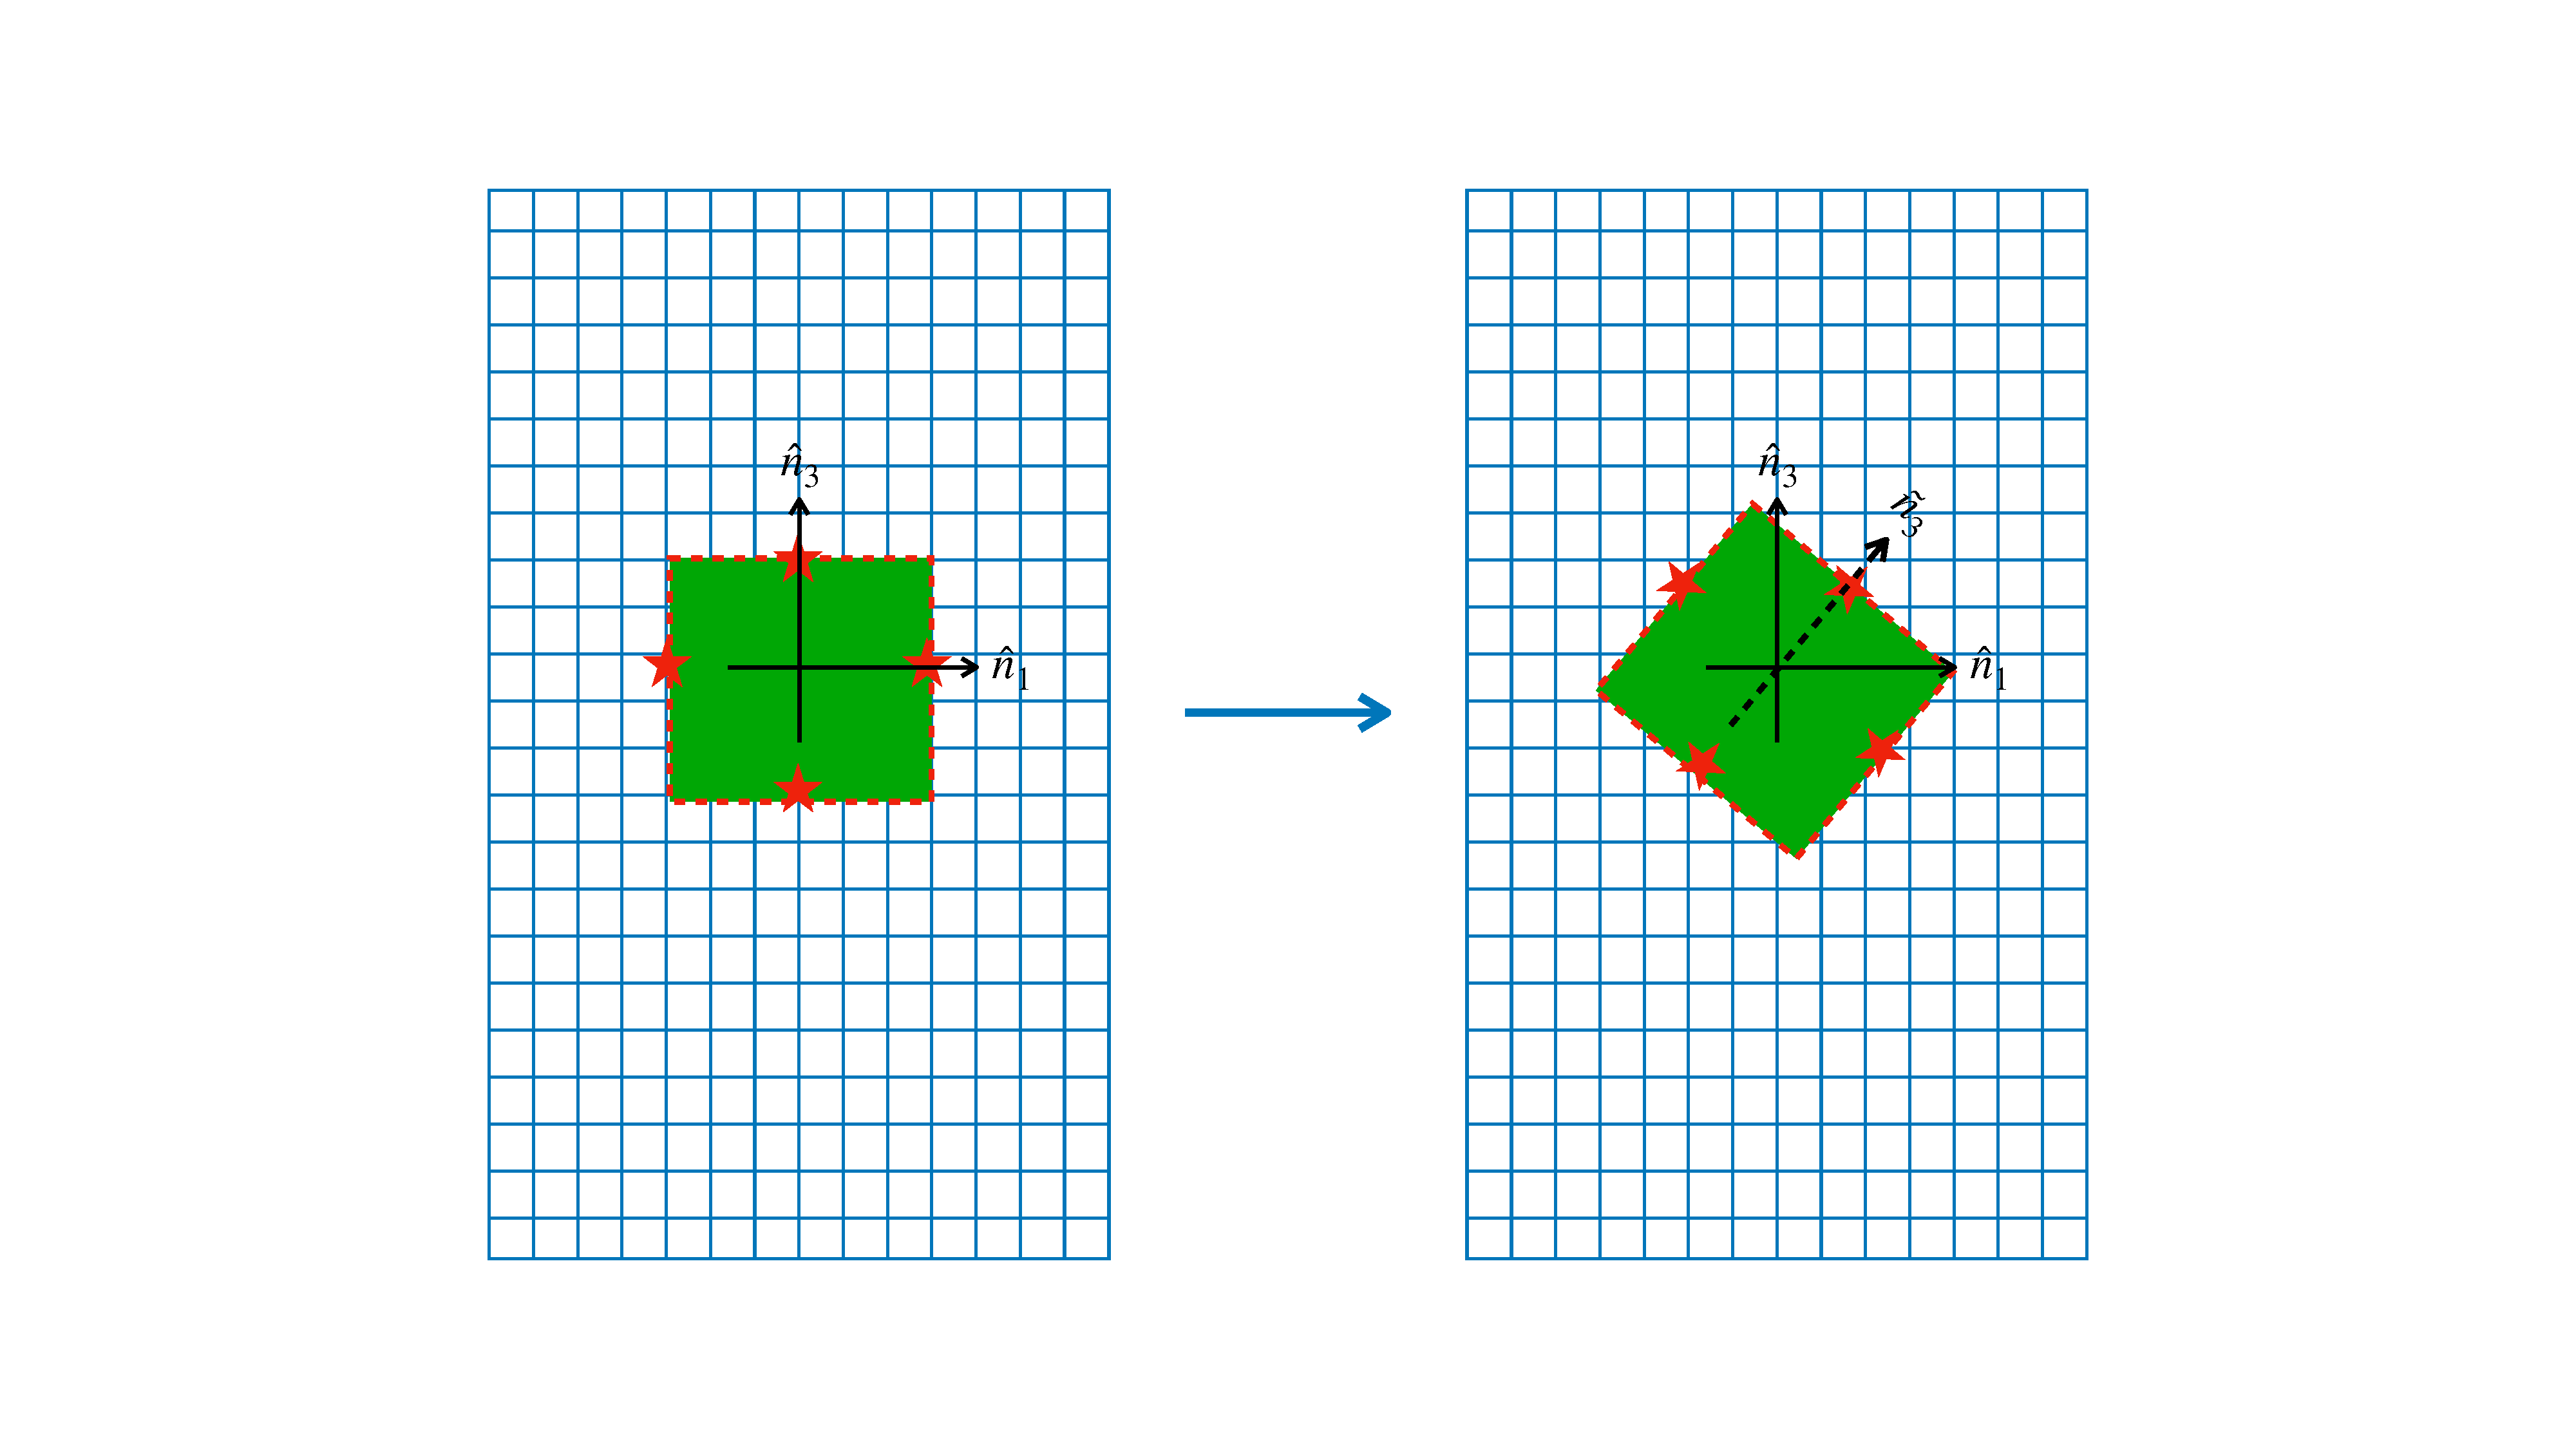
\includegraphics[scale=0.25]{./figures/fig_schematics}
		
    	\caption{Schematics of the rotation of aggregate.}
    	\label{fig_schematics}
    \end{center}
    \end{figure}
The points $\vec{y}$ are the blue grid in Figure \ref{fig_schematics} and the discretized version of $\vec{x}_s \in S$ are, in particular, the center of each square face. These are shown with red stars. We let the left-side plot in Figure \ref{fig_schematics} is the grid at time $t_n$ and the one after arrow shows the grid at time $t_n + \Delta t$.
\par
(Within a time step) When we solve for stress, $\vec{f}(\vec{x}_s)$, we also find aggregate's translational and angular velocities. For rotation, we focus on the angular velocity, $\vec{\Omega} \ \left(= \frac{\Delta \theta}{\Delta t}\right)$, which tells us how much the aggregate rotates. This information lives in $\mathcal{Q}(t)$, that is the orientation matrix, 
\[
{\color{blue}
\vec{x}_s(t) = \mathcal{Q}(t) \vec{x}.
}
\]
\subsection{Rotation matrix}
To move on to the next time step ($+ \Delta t$), we update the grid points with the velocity of the aggregate. Note that $\vec{U}_a$ and $\vec{\Omega}$ are translational and angular velocity. We focus on the rotation in this section. With the angular velocity and the time step, we find $\Delta t \vec{\Omega} = \left( \Delta \theta_1, \ \Delta \theta_2, \ \Delta \theta_3 \right) \equiv \Delta \vec{\theta}$, that is a three-dimensional change of angular position vector. 
The matrix $\mathcal{A}$ is then defined as 
\begin{equation}
	\mathcal{A}
	=\begin{bmatrix}
	 0 & - \Delta \theta_3 & \Delta \theta_2  \\
	 \Delta \theta_3 & 0  & -\Delta \theta_1  \\
	 - \Delta \theta_2 & \Delta \theta_1 & 0  \\
	\end{bmatrix},
	\label{eq_rotation_mx}
\end{equation}
From here, we have the rotation matrix $\mathcal{R} = e^{\mathcal{A}}.$
We can compute the matrix exponential $e^{\mathcal{A}}$ using Rodrigues' formula,
\begin{equation}
	\mathcal{R} = 
e^{\mathcal{A}} 
 = \bar{\bar{I \ }} 
 + \frac{\sin(\phi)}{\phi} \mathcal{A}
 + \frac{1-\cos(\phi)}{\phi^2} \mathcal{A}^2,
\label{eq_R_eA}
\end{equation} 
where $\phi = \|\Delta \vec{\theta}\|_2$.
With this $\mathcal{R}$ and orientation matrix $\mathcal{Q}$, we are ready to update fluid grid.


	
\subsection{Solve for stress}
We first solve for the stress on each square face of an aggregate, $\vec{y} = \vec{x}^*_s$, 
using the same formula as equation (\ref{eq_slp_nonD}),
\begin{equation}
	\vec{u} \left(\vec{x}^*_s ,t\right) 
		  = -\int_{S}  
		 \vec{f}(\vec{x}^*_s) 
		 \cdot \bar{\bar{G \ }} (\vec{x}_s,\vec{x}^*_s) 
		 \ \textrm{d}S(\vec{x}_s) 
		 + \frac{ \alpha C_{max}}{8\pi } \frac{\rho_0}{(\rho_s - \rho_0)(1-\phi)}
		 \int_V  C \left(\vec{x} ,t \right) \hat{k} \cdot
		 \bar{\bar{G \ }}(\vec{x}, \vec{x}^*_s)
		 \ \text{d}V(\vec{x}),
	\label{eq_slp_On}
\end{equation}
where the {\it Stokeslet} $\bar{\bar{G \ }}$ is defined as
\begin{equation}
	\bar{\bar{G}}( \vec{x}_s, \vec{x}^*_s) = 
	\frac{\bar{\bar{I \ }}}{||\vec{x}_s-\vec{x}^*_s ||} + \frac{(\vec{x}_s-\vec{x}^*_s)(\vec{x}_s-\vec{x}^*_s)^T}{||\vec{x}_s-\vec{x}^*_s ||^3}
	.
	\label{eq_stokeslet_star}
\end{equation} 
Note that $\vec{x}^*$ represents the center of a square face. 
\par
Equivalently, we can write equation (\ref{eq_slp_On}) as
\begin{equation}
	\vec{u} \left(\mathcal{Q} \vec{x}^* ,t\right) 
		  =- \frac{1}{8 \pi} \int_{S}  
		 \vec{f}(\mathcal{Q} \vec{x}) 
		 \cdot \bar{\bar{G \ }} (\mathcal{Q} \vec{x},\mathcal{Q}\vec{x}^*) 
		 \ \textrm{d}S(\vec{x}_s) 
		 - \frac{ \alpha C_{max}}{8\pi } \frac{\rho_0}{(\rho_s - \rho_0)(1-\phi)}
		 \int_V  C \left(\vec{x} ,t \right) \hat{k} \cdot
		 \bar{\bar{G \ }}(\vec{x}, \mathcal{Q} \vec{x}^*)
		 \ \text{d}V(\vec{x}).
	\label{eq_slp_On_rotate}
\end{equation}
One can see that it is valid to say
\[
	\bar{\bar{G}}( \vec{x}_s, \vec{x}_s^*)
	= \bar{\bar{G \ }} (\mathcal{Q} \vec{x},\mathcal{Q}\vec{x}^*) 
	 = \bar{\bar{G}}( \vec{x}, \vec{x}^*)
\]
since the rotation matrix $Q$ is constant and it is normalized. 
Precisely, we use the following form in Matlab program:
\begin{equation}
	\vec{u} \left(\mathcal{Q} \vec{x}^*\right) 
		  + \frac{1}{8 \pi} \int_{S}  
		 \vec{f}(\mathcal{Q} \vec{x}^*) 
		 \cdot \bar{\bar{G \ }} (\vec{x},\vec{x}^*) 
		 \ \textrm{d}S(\vec{x}_s) 
		 =
		 - \frac{ \alpha C_{max}}{8\pi } \frac{\rho_0}{(\rho_s - \rho_0)(1-\phi)}
		 \int_V  C \left(\vec{x} ,t \right) \hat{k} \cdot
		 \bar{\bar{G \ }}(\vec{x}, \mathcal{Q} \vec{x}^*)
		 \ \text{d}V(\vec{x}).
	\label{eq_slp_stress_aggR}
\end{equation}

We see that LHS has unknowns including the translational and angular velocities
in $\vec{u}\left(\mathcal{Q} \vec{x}^* ,t\right)$.
Note that the stress values we obtain here 
are located in the same one as the rotated positions.  
We also want to point out that the target points in the volume integral
are the center of square faces after rotation, $\mathcal{Q}\vec{x}^*$.
\par
In order to build the linear system with the boundary integral computed in the
 fixed grid, we should map the value of the volume integral and drag $\vec{F}_o$ into 
 the same coordinate system, temporarily. 
We simply can muptipliy by $\mathcal{Q}^{-1} = \mathcal{Q}^{T}$ to do this job.
\begin{equation}
	\mathcal{Q} 
	\left[\vec{u} \left( \vec{x}^* \right) 
		  + \frac{1}{8 \pi}   \int_{S}  
		 \vec{f}( \vec{x}^*) 
		 \cdot \bar{\bar{G \ }} (\vec{x},\vec{x}^*) 
		 \ \textrm{d}S(\vec{x}_s) 
		 \right]
		 =
		 - \frac{ \alpha C_{max}}{8\pi } \frac{\rho_0}{(\rho_s - \rho_0)(1-\phi)}
		 \int_V  C \left(\vec{x} ,t \right) \hat{k} \cdot
		 \bar{\bar{G \ }}(\vec{x}, \mathcal{Q} \vec{x}^*)
		 \ \text{d}V(\vec{x}).
	% \label{eq_slp_stress_aggR}
\end{equation}
The following equivalent euation is implemented in Matlab code:
\begin{equation}
	 \vec{u} \left( \vec{x}^* \right) 
		  + \frac{1}{8 \pi}   \int_{S}  
		 \vec{f}( \vec{x}^*) 
		 \cdot \bar{\bar{G \ }} (\vec{x},\vec{x}^*) 
		 \ \textrm{d}S(\vec{x}_s) 
		 =
		 \mathcal{Q}^{-1}
		 \left[
		 - \frac{ \alpha C_{max}}{8\pi } \frac{\rho_0}{(\rho_s - \rho_0)(1-\phi)}
		 \int_V  C \left(\vec{x} ,t \right) \hat{k} \cdot
		 \bar{\bar{G \ }}(\vec{x}, \mathcal{Q} \vec{x}^*)
		 \ \text{d}V(\vec{x})
		 \right]
		 .
	% \label{eq_slp_stress_aggR}
\end{equation}
Note that 
\[
\vec{u}(\vec{x}^*)
 = \vec{U}_a + \vec{\Omega} (\vec{x}^* - \vec{x}_{cm}).	
\]
%
% I understand that the notations are confusing; The simplest way to read them is 
% that no subscription of $s$ means that the point is staying in Cartesian grid as fluid coordinates. 
%
\par
The main part to compute the drag $\vec{F}_o$ is in the density of the fluid
 \begin{equation}
	 \rho (\vec{x}, t_n + \Delta t) = 
	 \rho_{bg} + \rho_C =
	 \rho_0 \biggl( 1 + \gamma z \biggr)   + \rho_0 \biggl( \alpha C_{max} C(\vec{x}, t_n + \Delta t) \biggr),
\end{equation}
when $\vec{x} = (x, y, z)$. 
\\
After we get the new density, we prepare to build the linear system to obtain next time-step stress with the following two more equations of the drag and torque,
\begin{equation}
\int_{S} \vec{f}(\vec{x}_s) \  \text{d}S(\vec{x}_s)
= \vec{F}_o
 \label{eq_drag}
 \end{equation} 
 \begin{equation}
 	\int_S \vec{f} (\vec{x}_s)  \times (\vec{x}_s - \vec{x}_{cm}) \ \textrm{d}S(\vec{x}_s) = \vec{Q}_o.
 \label{eq_torque}
 \end{equation}
 where 
  \begin{equation}
	  \vec{F}_o = 
 \frac{g}{\mu U_s L}
	\left( 
	- \rho_a V_a \hat{k}
	+ \int_{S} \left( 
	   \int  {\rho}_{bg}(z) \ \textrm{d}z
	 \right) 
	\hat{n} \ \textrm{d}S (\vec{x})
	\right),
	 \label{eq_Fo_2}
\end{equation}
where 
\[
\rho_a = \frac{\phi}{V_a}\int_{V_a} \rho(\vec{x}) \ \text{d}V
+ (1-\phi)\rho_s.
\]
Note that $\phi$ and $\rho_s$ represents constant porosity and 
solid portion of the aggregate.
We see that the LHS of both equations (\ref{eq_drag}) 
and (\ref{eq_torque}) are solved in the aggregate grid. 
The RHS of equation (\ref{eq_drag}) is a combination of body force and buoyancy.
To calculate the aggregate density, $\rho_a$, numerically, 
we sum up all the background density where the cubes are located. 
For the buoyancy force as well, the center of each cube is required information.
We thus need to use the rotated aggregate position, $\vec{x}_s$.  
For this reason, what we implement in Matlab code is the following:
\begin{equation}
	\int_{S} \vec{f}(\vec{x}) \  \text{d}S(\vec{x})
	= \mathcal{Q}^{-1} \vec{F}_o
	 \label{eq_drag_code}
	 \end{equation} 
	 \begin{equation}
		 \int_S \vec{f} (\vec{x})  \times (\vec{x} - \vec{x}_{cm}) 
		 \ \textrm{d}S(\vec{x}) 
		 = (0,\ 0, \ 0).
	 \label{eq_torque_code}
	 \end{equation}
\par
Once we solve the linear system ,
 we may put the unknow values into the correct location.
We need to rotate them using
\[
\vec{f}(\vec{x}_s) = \mathcal{Q} \vec{f}(\vec{x}).	
\]
\[
\vec{U}_a (\vec{x}_s) = \mathcal{Q} \vec{U}_a (\vec{x}).	
\]
\[
\vec{\Omega}(\vec{x}_s) = \mathcal{Q} \vec{\Omega}(\vec{x}).	
\]
The validation of stress is in section (\ref{validation_rot}).


\subsection{Velocity field}
Once we solve for the stress, we use the same 
equation (\ref{eq_slp_nonD}) 
to solve for velocity on the fluid grid which stays in the Cartesian coordinates, 
$\vec{y}$,
\begin{equation}
	\vec{u} \left(\vec{y},t\right) 
		  =- \frac{1}{8 \pi} \int_{S}  
		 \vec{f}(\vec{x}_s) 
		 \cdot \bar{\bar{G \ }} (\vec{x}_s,\vec{y}) 
		 \ \textrm{d}S(\vec{x}_s) 
		 + \frac{ \alpha C_{max}}{8\pi } \frac{\rho_0}{(\rho_s - \rho_0)(1-\phi)}
		 \int_V  C \left(\vec{x} ,t \right) \hat{k} \cdot
		 \bar{\bar{G \ }}(\vec{x}, \vec{y} )
		 \ \text{d}V(\vec{x}).
\end{equation}
The volume integral term does not need any special treatment. 
However, the boundary integral needs some work
since we have two different coordinates systems are mixed.
Assume that $\vec{f}(\vec{x}_s)$ is constant for each square face. 
We here investigate more integral of the kernel,
\[
	\bar{\bar{G \ }} (\vec{x}_s,\vec{y}) 
		 \ \textrm{d}S(\vec{x}_s)
	= 
	\frac{\bar{\bar{I \ }}}{||\vec{x}_s-\vec{y} ||} 
	+ \frac{(\vec{x}_s-\vec{y})(\vec{x}_s-\vec{y})^T}{||\vec{x}_s-\vec{y} ||^3}, 	 
\]
where $\vec{y}$ is in Cartesian coordinate 
and $\vec{x}_s$ is in aggregate grid which is (possibly) rotated. 
The challenge part here is that 
our Matlab program to compute this boundary integral of $\bar{\bar{G}}$
is set in the Cartesian coordintes. 
We thus would like to express the $\vec{v} = \vec{x}_s - \vec{y}$ 
in the Cartesian grid, i.e., we find the same vector $\vec{v}$ in fluid coordintate.
{\color{blue} Need to type below figure.}
\begin{figure}[h]
	\begin{center}
		\includegraphics[scale=0.45]{./figures/fig_vel_y_map}		
		\caption{Mapping for $\vec{y}$ grid.}
		\label{fig_vel_y_map}
\end{center}
\end{figure}

After we solve for the velocity field of the fluid domain at time $t = t_n$ and translational $\&$ angular velocities, we first obtain new perturbation at time $t = t_n + \Delta t$, in the moving frame of reference. This involves only the translational velocity,     $\vec{U}_a$, with the velocity field (Not the grid points). 
Once we obtain the $C(\vec{x}, t+\Delta t) $, we use this value to update the density of the fluid.
%
\subsection{Update perturbation}
Since we calculate the perturbacion, $C(\vec{x},t)$ in the moving fram of reference, 
we use the translational velocity, $\vec{U}_a$, to move aggregate back to the center of 
fluid domain.
In the same manner, we may need to rotate the velocity field back to the moving frame 
by multiplying by inverse of $\mathcal{Q}$ temporarily. 
\clearpage
\subsection{Validations}\label{validation_rot}
We first test the implementation of rotation with zero perturbation, i.e.,  $C(\vec{x}) = 0$ for all $\vec{x}$. 
We still have a light density gradient in the background ($\gamma = - 0.001$). Suppose that we have an aggregate with three cubes 1) vertically and 2) horizontally stacked. See Figure \ref{fig_NC3_hor_vert}. We found these two models by setting the random seed numbers (left) 6 and (right) 99, in \verb+DLA_3D+ function. 
    \begin{figure}[h]
    	\begin{center}
    		\vspace{0.5cm}
			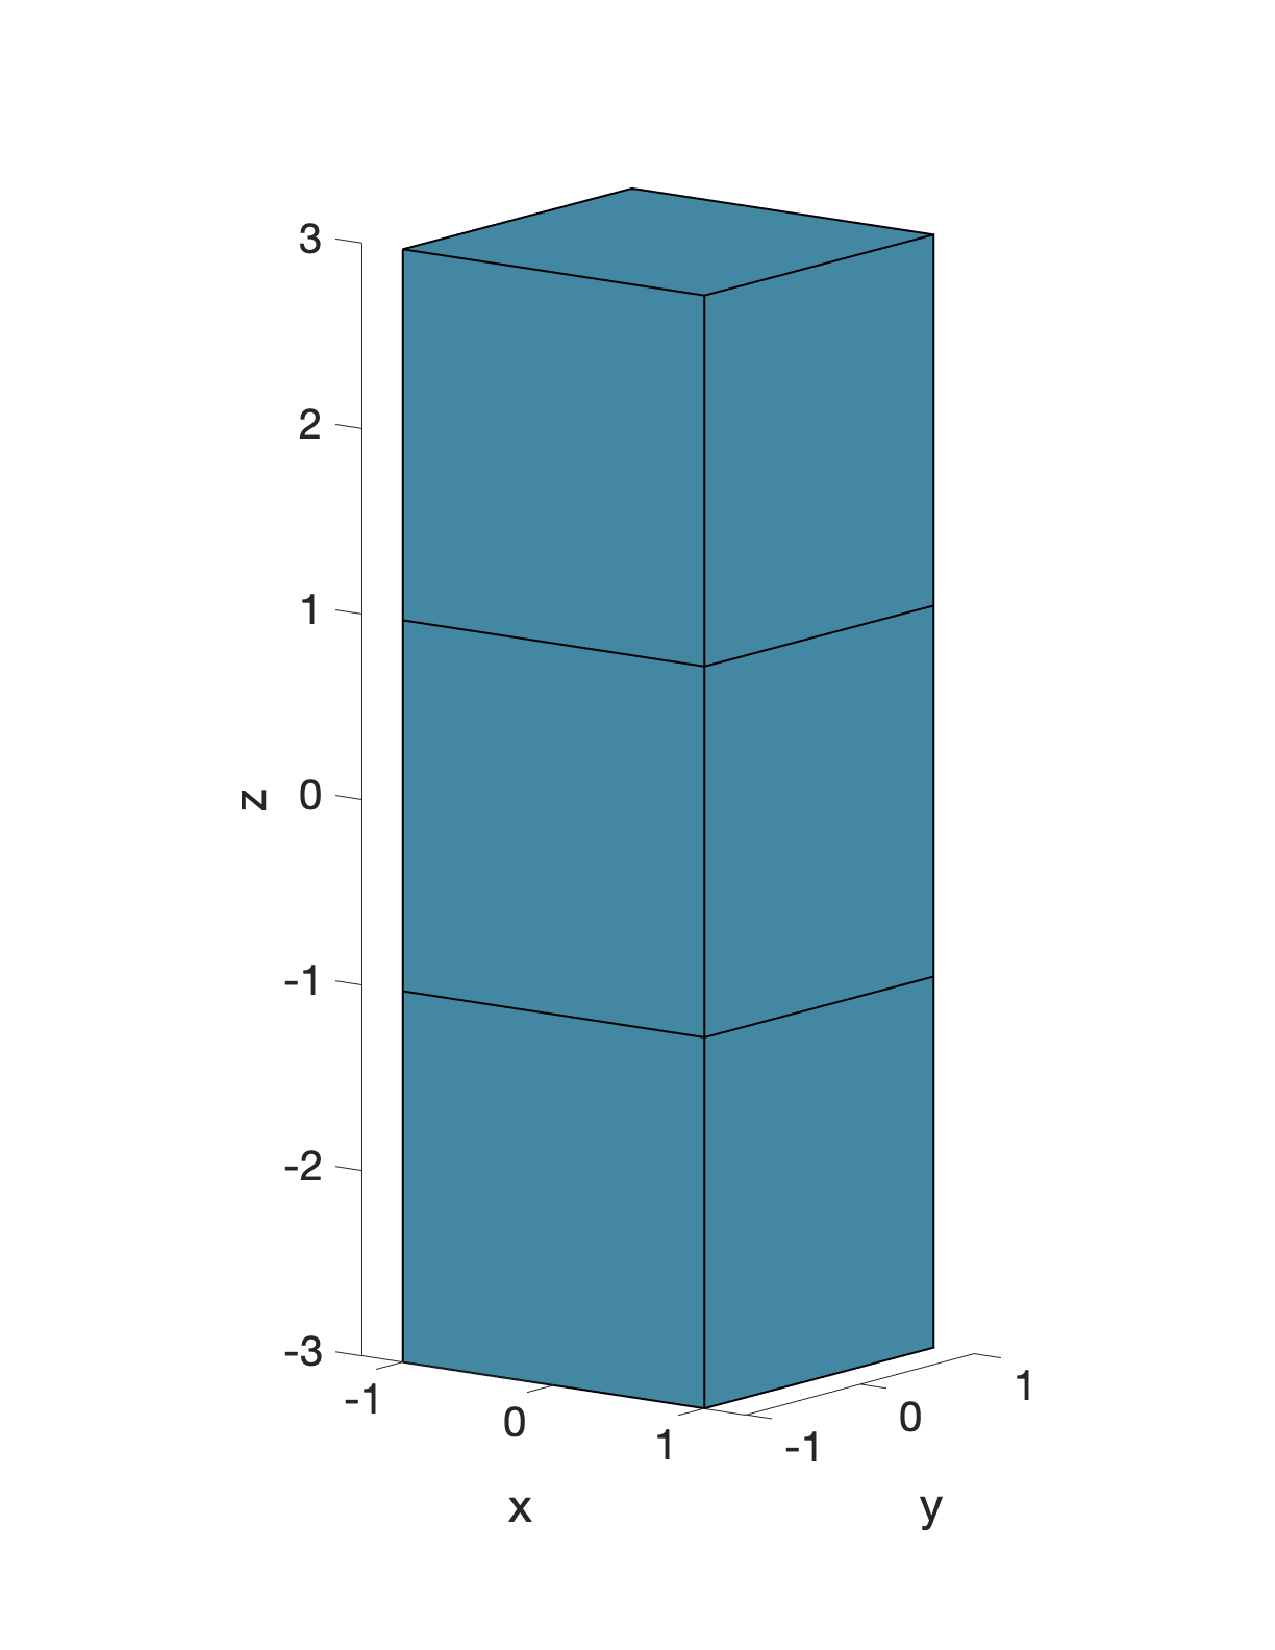
\includegraphics[scale=0.25]{./figures/fig_NC3_ver}		
			\hspace{20mm}
			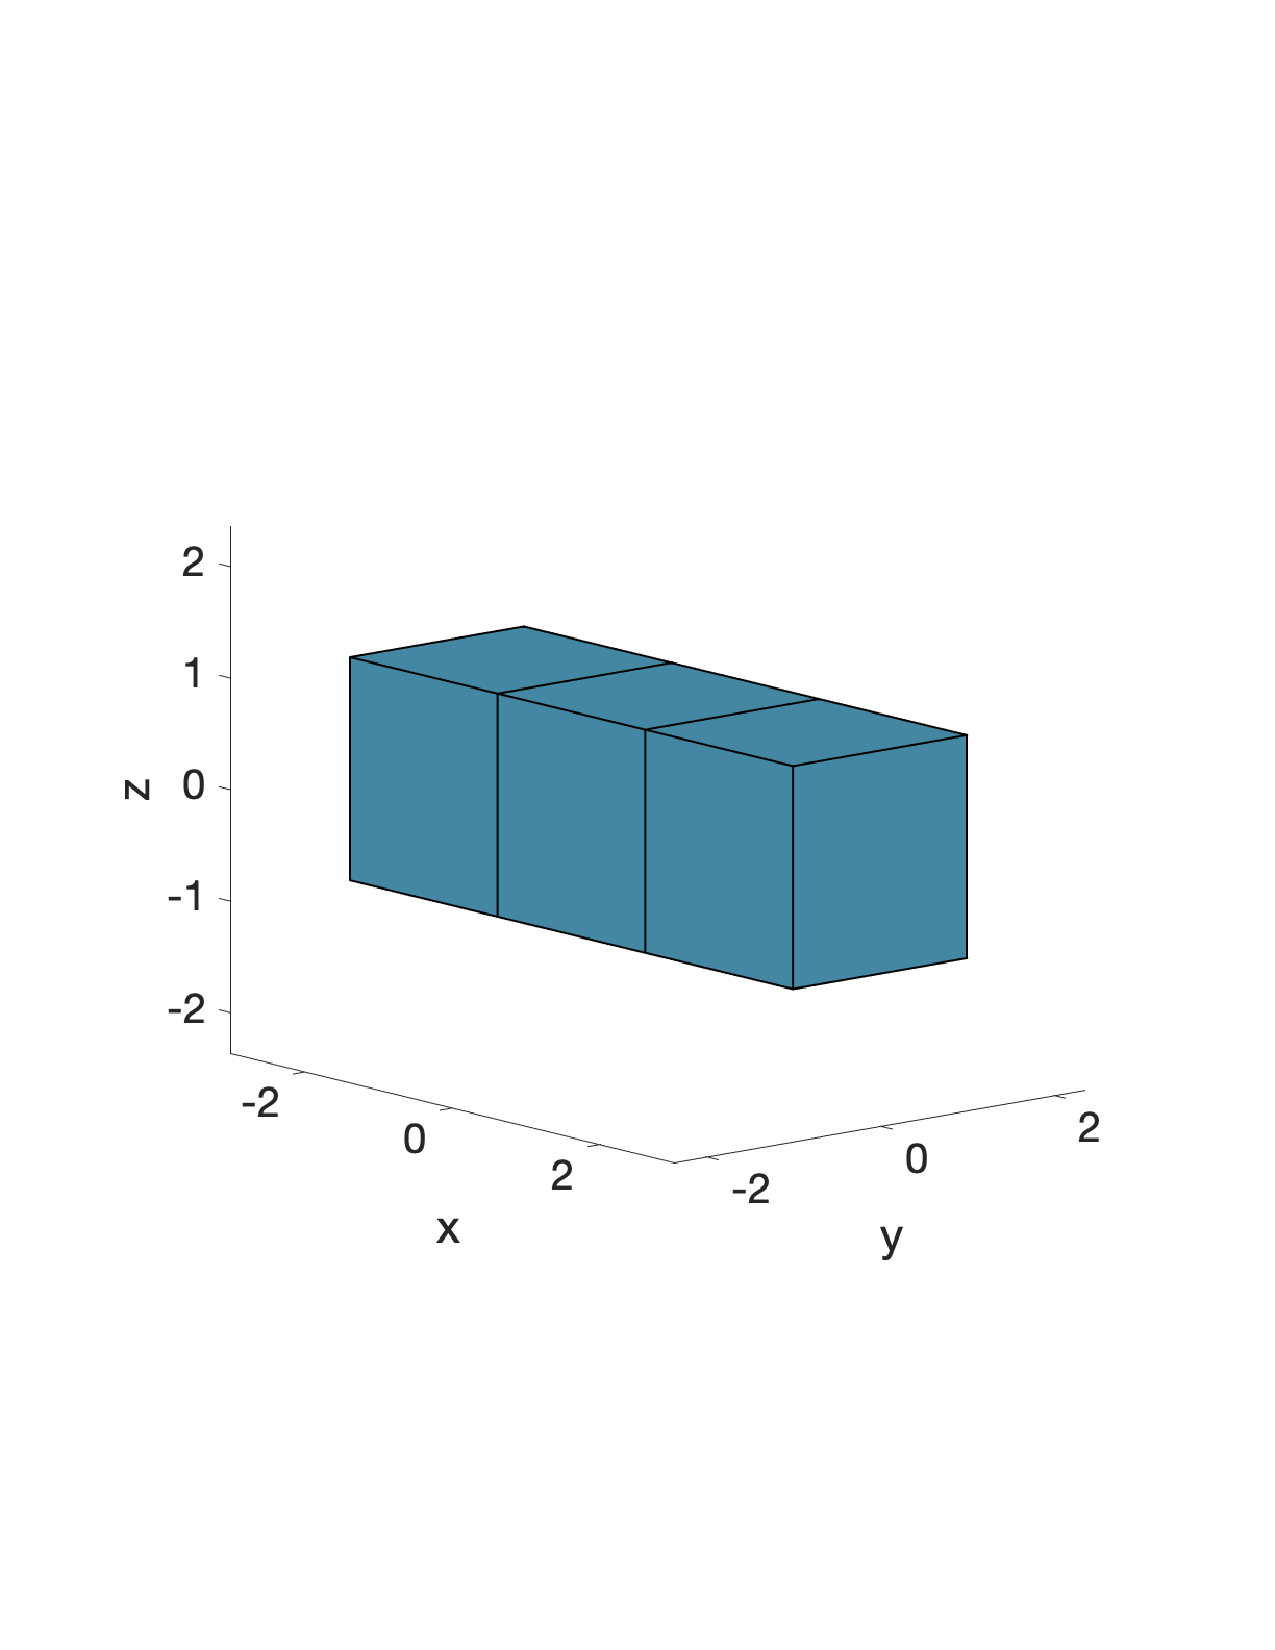
\includegraphics[scale=0.35]{./figures/fig_NC3_hor}		
    	\caption{Aggregate made with three cubes; (Left) vertically and (Right) horizontally stacked.}
    	\label{fig_NC3_hor_vert}
    \end{center}
\end{figure}
\\
Both aggregates are centered at origin, $\vec{x}_{cm} = (0,0,0)$.
We see that the horizontal aggregate (right) can be obtained by rotating the vertical one (left) 90-degrees around the $y$ axis. This implies that when we compute the forces, such as drag and stress, of the vertical aggregate after the 90-degrees rotation, the values should match with the horizontal aggregate case. Note that we only rotate the vertical aggregate to compare force values. 
\\
We set \verb+Omega = [0; pi/2; 0]+ as the aggregate's angular velocity. We then apply this to find the rotation matrix $\mathcal{R}$ using equation (\ref{eq_R_eA}). In Matlab program, we actually rotate the fluid domain, not the aggregate directly. This can be simply done by applying transpose of $\mathcal{R}$ to the fluid grid. 
\begin{framed}
	\verb+xyz_R = Qtp1' * (xyz - cm_0)+
\end{framed}
\noindent
Here, \verb+Qtp1+ represents $R Q(t)$, where $Q(t)$ is initially identity matrix as we begin with Cartesian coordinate. Also, \verb+cm_0+ is the center of mass, $\vec{x}_{cm}.$
\par
We first compute the drag, $\vec{F}_o$, using equation (\ref{eq_Fo}). In Matlab, we do not need the rotated grid for buoyancy force, the integral tern in equation (\ref{eq_Fo}). However, we need fluid density for the body force. In particular, the aggregate density, $\rho_a$, requires fluid density inside of the aggregate. 
    \begin{figure}
    	\begin{center}
			\includegraphics[scale=0.3]{./figures/fig_stress_hor_NoR}
    	\caption{Stress on horizontal aggregate without rotation.}
    	\label{fig_stress_hor_NoR}
    \end{center}
    \end{figure}
	% After rotation
    \begin{figure}
    	\begin{center}
			\includegraphics[scale=0.3]{./figures/fig_stress_vert_R}
    	\caption{Stress on vertical aggregate after 90-degreses rotation around $y-$ axis.}
    	\label{fig_stress_vert_R}
    \end{center}
    \end{figure}
% \subsection{Validation: Rotation around the vertical axis}
\par
Next, we test the implementation of rotation with zero perturbation, 
i.e.,  $C(\vec{x}) = 0$ for all $\vec{x}$. 
We still have a light density gradient in the background ($\gamma = - 0.001$). 
Suppose that we have two aggregates with three cubes stacked horizontally.
The only difference between them is that one is rotated around $z-$axis. 
See Figure \ref{fig_NC3_hor_92}. 
We found these two models by setting the random seed numbers (left) 99 
and (right) 92, in \verb+DLA_3D+ function. 
    \begin{figure}[h]
    	\begin{center}
    		\vspace{0.5cm}
			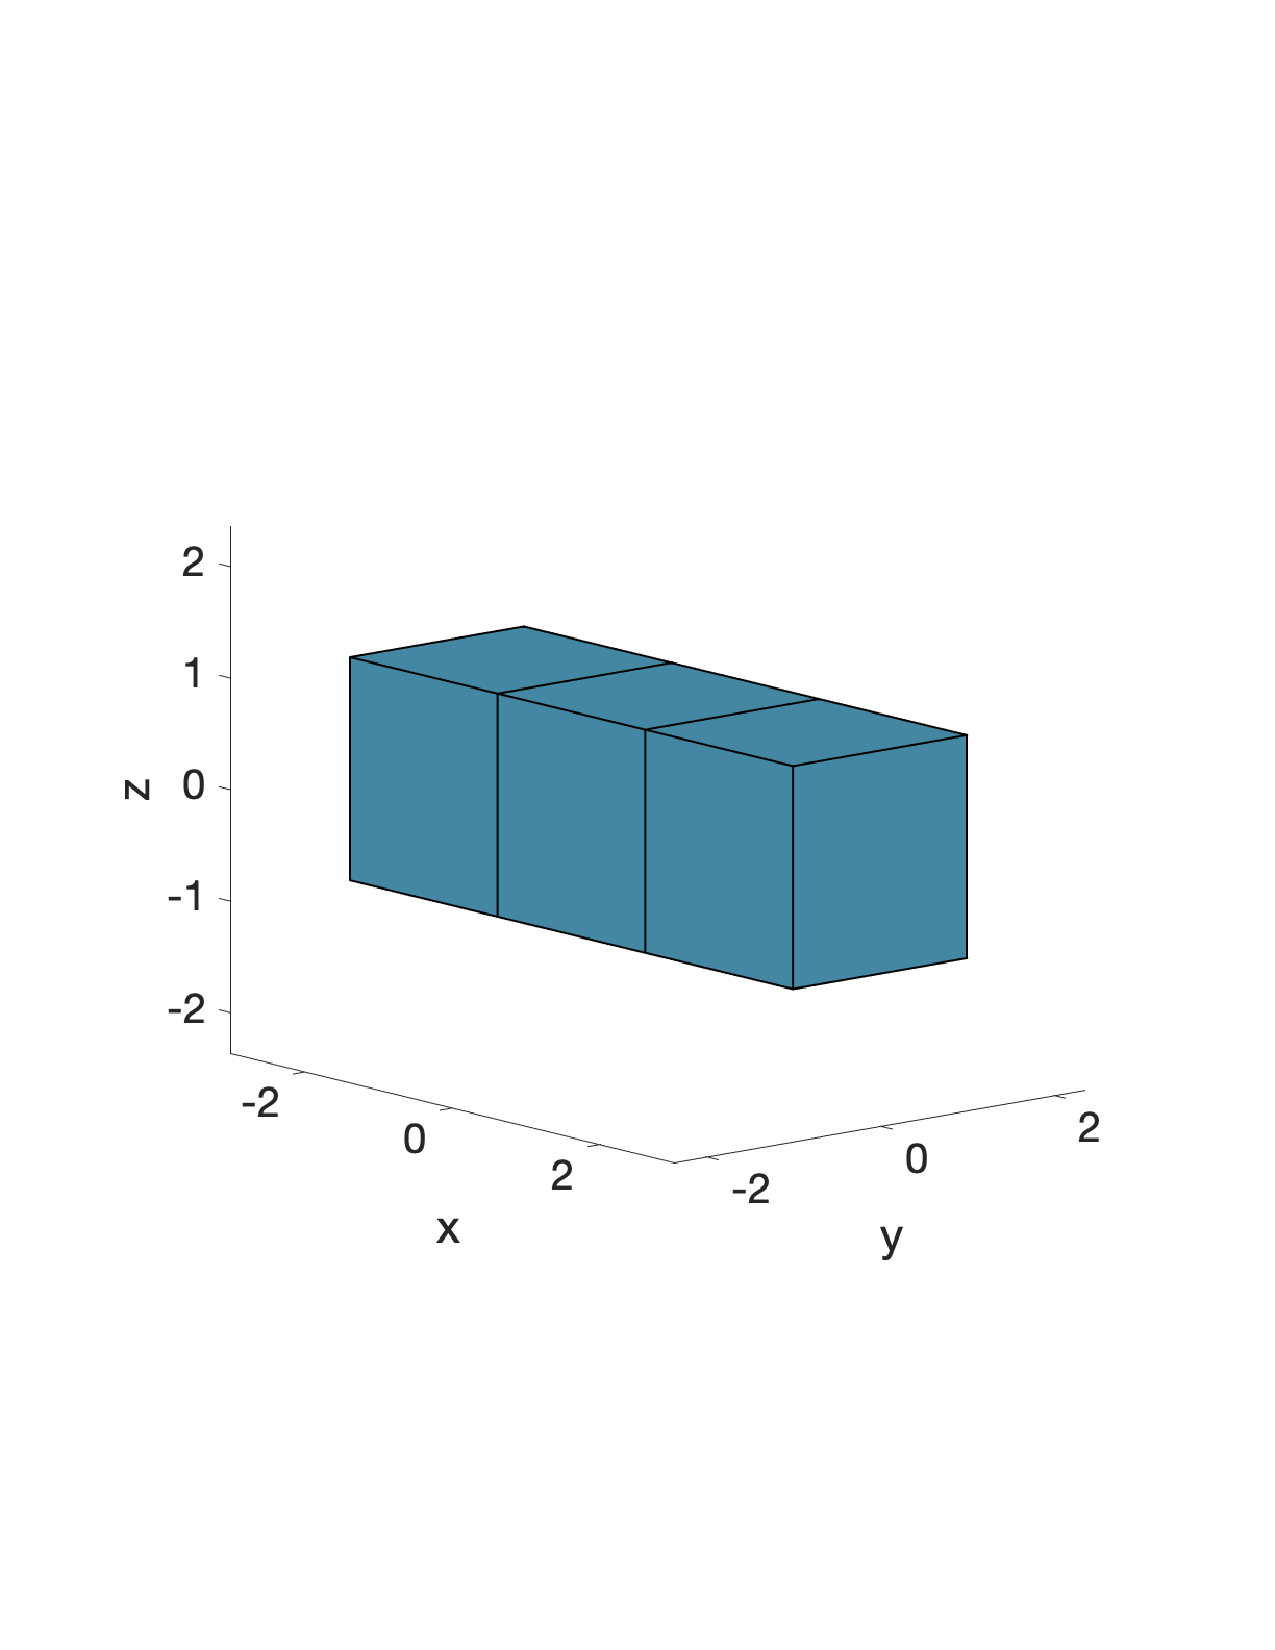
\includegraphics[scale=0.35]{./figures/fig_NC3_hor}		
			\hspace{20mm}
			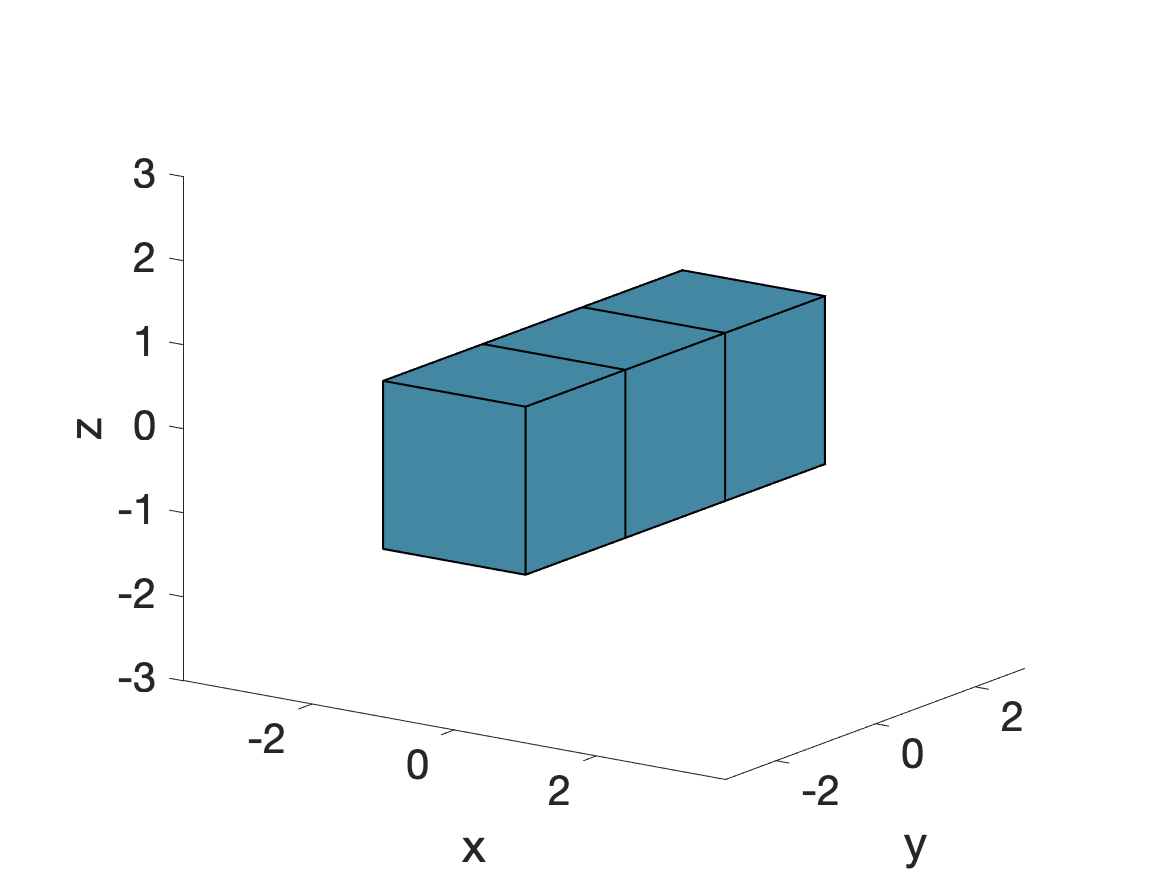
\includegraphics[scale=0.38]{./figures/fig_NC3_hor92}		
    	\caption{Aggregate made with three cubes horizontally stacked.}
    	\label{fig_NC3_hor_92}
    \end{center}
\end{figure}
We compare the stress on each face in the same manner we showed in the precious section.
For this validation, we add initial pertubation $C(\vec{x})$ with a Gaussian function;
\[
C(x,y,z) =  10^{-3} e^{-(1/3)\left(x^2 + y^2 + z^2\right)}.
\]
%before rotation
    \begin{figure}
    	\begin{center}
			\includegraphics[scale=0.35]{./figures/fig_stress_NoR_99}
    	\caption{Stress on horizontal aggregate without rotation.}
    	\label{fig_stress_NoR_99}
    \end{center}
    \end{figure}
	% After rotation
    \begin{figure}
    	\begin{center}
			\includegraphics[scale=0.35]{./figures/fig_stress_R_92}
    	\caption{Stress on horizontal aggregate after 90-degreses rotation around $z-$ axis.}
    	\label{fig_stress_R_92}
    \end{center}
    \end{figure}

% For furture validation of implementation, 
% we use non-symmetric Gaussian function as an initial perturbation,
% \[
% C(\vec{x}) = 
% \exp{(-(1/3)((x-1.3)^2 + (y-0.5)^2 + z^2))} \times 10^{-3}.	
% \]
% \begin{figure}[h]
% 	\begin{center}
% 		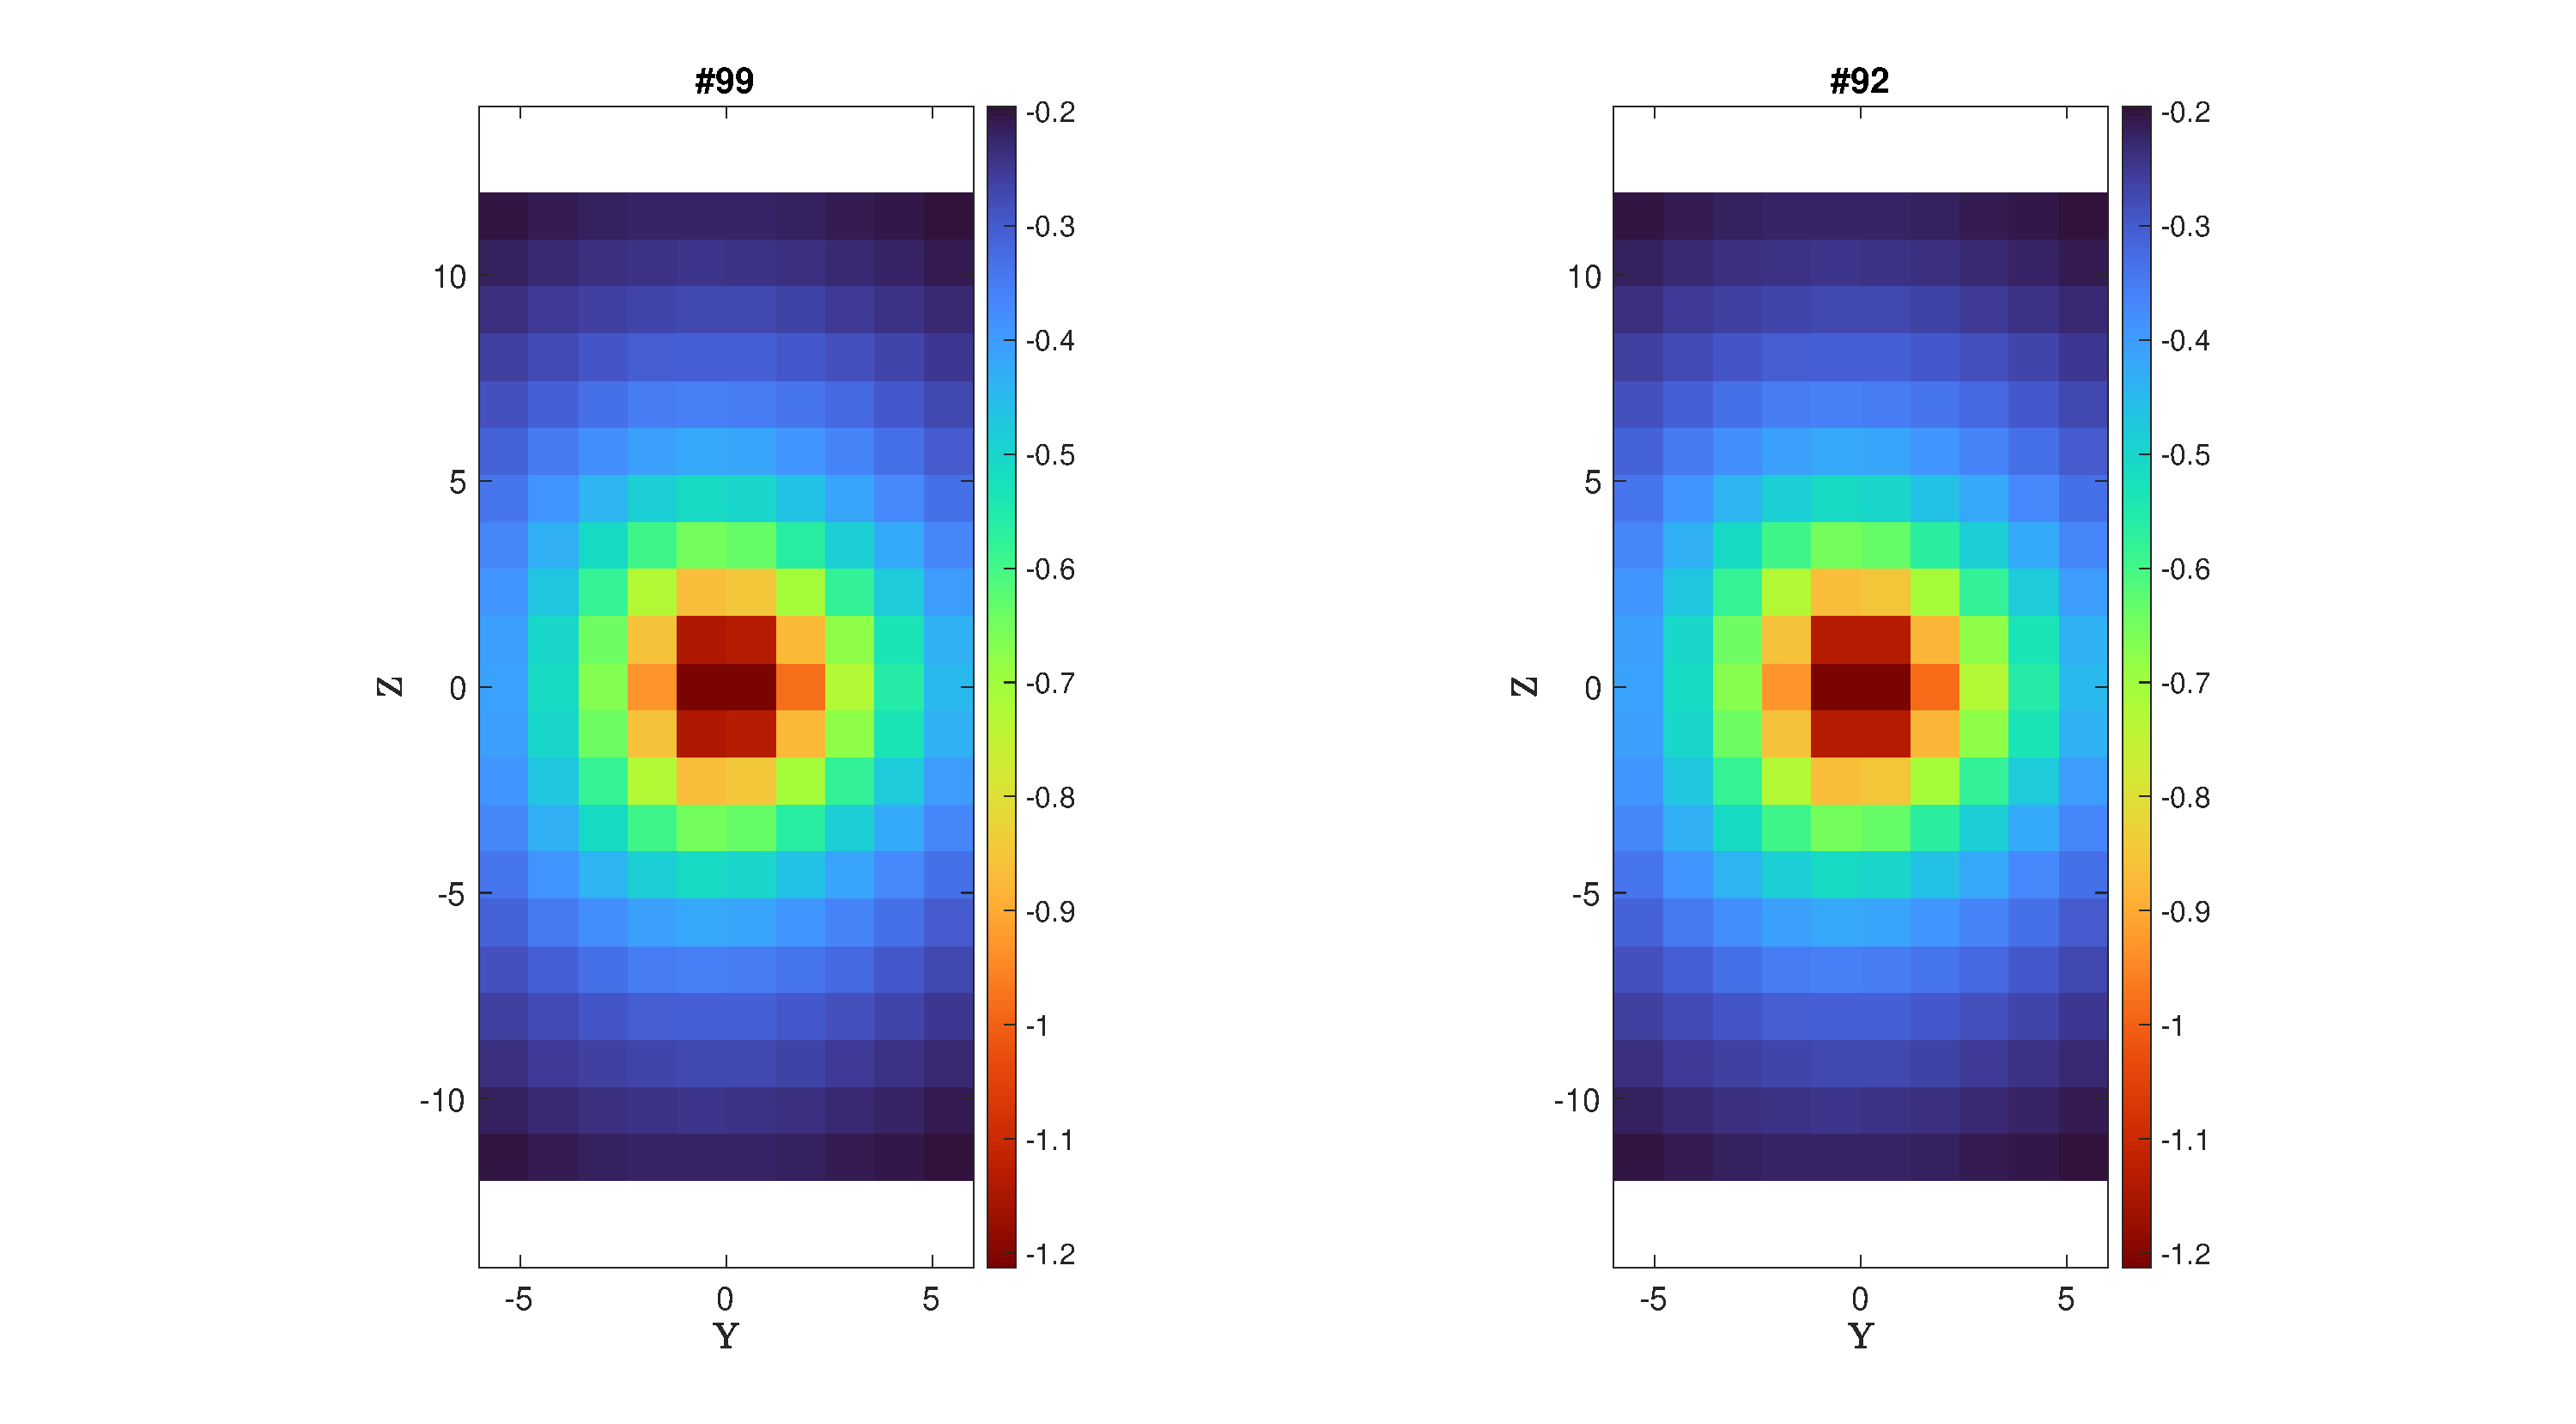
\includegraphics[scale=0.35]{./figures/fig_velZ_99_92R_xp06}
% 	\caption{veloity in $z$ direction at $x = 0.06$.}
% 	\label{fig_velZ_99_92R_xp06}
% \end{center}
% \end{figure}
% %------------------------------Numerics--------------------------------------
\section{Numerical methods}
%------------------------------------------------------------------
*We drop the prime for all dimensionless equations. 
\\
In this section, we explain the details of numerical methods. We first consider the background fluid density that is a part of the drag computation. We derive the simplest form to implement in codes. We then discuss the homogeneous velocity field. We compare two boundary integral equations since it was not straightforward to choose one. Lastly, we present the method to compute the non-homogeneous solution which is a volume integral of the perturbation $C(\vec{x},t)$. Due to the high computational cost, we use the fast multipole method (FMM). We give a brief introduction of the FMM and framework for Stokes kernel.
 \subsection{Background fluid density}
In this section, we explain how to compute the (dimensional) buoyancy term in equation, that is
\begin{equation}
	\rho_{by} =
	 \int_{S} \left( 
	   \int  {\rho_{bg}} (z) g \ \textrm{d}z
	 \right) \bar{\bar{I \ }}  \cdot
	\hat{n} \ \textrm{d}S (\vec{x}).
\label{eq_buoyancy2}
\end{equation}
We consider a single cube case for simplicity, i.e., $Nf = 6$. We can simply extend it to multiple cubes in the same manner. The discretized version of integral (\ref{eq_buoyancy2}) is 
\begin{equation}
	\sum_{i=1}^{Nf}
	 L^3 \int_{S^i} \left( 
	   \int  {\rho_{bg}} (z) g  \ \textrm{d}z 
	 \right) \bar{\bar{I \ }}  \cdot
	\hat{n}_i \ \textrm{d}S^i (\vec{x}),
\label{eq_buoyancy_discrete2}
\end{equation}
where $i$ represents the index of square faces (not a power). Note that we muptiply by $L^3$ to keep the dimensionality. Depending on the orientation of each square face, the integral domain or axis of $S^n$ is different. For example, let $S^1$ be the first square with the normal $\hat{n}_1 = (1,0,0)$. Then 
\begin{equation}
	L^3 
	 \int_{S^1}
	 \left( 
	   \int  {\rho_{bg}} (z) g \ \textrm{d}z 
	 \right) \bar{\bar{I \ }}  \cdot
	\hat{n}_1 \ \textrm{d}S^1 (\vec{x})
	= L^3  \int_{-1}^{1} \int_{-1}^{1}
	\left( 
  	 \int  {\rho_{bg}} (z) g \ \textrm{d}z 
 	\right) \bar{\bar{I \ }}  \cdot
 	\hat{n}_1 \ 
	\textrm{d}y  \textrm{d}z 
\label{eq_buoyancy_S1_2}
\end{equation}
Since the background function $\rho_{bg}$ is a function of $z$ only,intuitively, we see that the value (\ref{eq_buoyancy_S1_2}) and the one with the normal $\hat{n}_6 = -\hat{n}_1 = (-1,0,0)$ has the same magnitude but in the opposite direction. This means that when we add the integrals on $S^1$ and $S^6$, we get zero. We can also prove this with simple arithmetics. 
\par
We first write the inner integral explicitly using
\[
L^3 \int  {\rho_{bg}} (z)g  \ \textrm{d}z 
 =  L^3 \left( \rho_0 \int  1+\gamma  z \right) g \ \textrm{d}z 
=L^3 \rho_0 \left(  z + \frac{\gamma}{2}z^2 + c \right) g,
\]
where $c$ is an integral constant. This form is valid for any $z$. The surface integral on $S^1$ then becomes 
\[
	L^3\rho_0  \int_{-1}^{1} \int_{-1}^{1}
  	\left( 
  	 z + \frac{\gamma}{2}z^2 + c 
 	\right) g \bar{\bar{I \ }}  \cdot
 	\hat{n}_1 \ 
	\textrm{d}y  \textrm{d}z 
	=
2L^3 \rho_0\hat{n}_1 
\int_{-1}^{1} 
  	\left( 
  	z + \frac{\gamma}{2}z^2 + c  
 	\right) g \ 
  \textrm{d}z 
  =4 L^3 \rho_0 \left( c + \frac{\gamma}{6} \right) g \hat{n}_1 .
\]
We see that the only difference we would get from the surface integrals for $S^1$ and $S^6$ is the direction of the normals. We can apply the same concept to the other two square faces, $S^2$ and $S^5$, in which their normals are $\hat{n}_2 = -\hat{n}_5 = (0,1,0)$. This implies that the only squares we need to pay attention are the rest of two faces that have normals parallel to $z-$axis. We denote these squares as $S^3$ and $S^4$ and their normals are $\hat{n}_3 = (0,0,1)$ and $\hat{n}_4 = -\hat{n}_{3}$, respectively. 
\par
The surface integral on $S^3$ is 
\[ L^3
\rho_0\int_{-1}^{1} \int_{-1}^{1}
  	\left( 
  	 z + \frac{\gamma}{2}{z}^2 + c 
 	\right)g  \bar{\bar{I \ }}  \cdot
 	\hat{n}_3 \ 
	\textrm{d}x  \textrm{d}y 
	% = 4\left(
%   	\int \rho_{bg}(z) \ \textrm{d}z
%  	\right)
%  	\hat{n}_3
	= 4 L^3 \rho_0 \left( z_T + \frac{\gamma}{2} {z_T}^{2} +c \right) g \hat{n}_3,
\]
where $z_T$ is the constant $z-$ value of the surface $S^3$ face (top face).
We can compute the surface integral on $S^4$ in the same manner. Then, the buoyancy equation (\ref{eq_buoyancy_discrete2}) becomes
\begin{equation}
	\sum_{i=1}^{6} L^3
	 \int_{S^i} \left( 
	   \int  {\rho_{bg}} (z)  \ \textrm{d}z 
	 \right) g \bar{\bar{I \ }}  \cdot
	\hat{n}_i \ \textrm{d}S^i (\vec{x})
	= 4 L^3 \rho_0 \left( z_T + \frac{\gamma}{2} {z_T}^{2} +c \right) g \hat{n}_3
	+ 4L^3 \rho_0 \left( z_B + \frac{\gamma}{2} {z_B}^{2} + c \right) g \hat{n}_4,
\label{eq_buoyancy_discrete_eval2}
\end{equation}
where $z_B$ is the constant $z-$ value of the surface $S^4$ (bottom face). By substituting the normals $\hat{n}_3$ and $\hat{n}_4$, we can simplify the right-hand side of equation (\ref{eq_buoyancy_discrete_eval2}), knowing that $z_T - z_B = 2$;
\begin{equation}
4 L^3 \rho_0 \left( z_T + \frac{\gamma}{2} {z_T}^{2} + c \right) g 
	- 4 L^3 \rho_0 \left( z_B + \frac{\gamma}{2} {z_B}^{2} + c \right) g
= 8 L^3 \rho_0 \left( 1+ \gamma (1+z_B) \right)g
= 8 L^3 \rho_0 \left( 1+ \gamma z_{c_n} \right) g , 
\label{eq_buoyancy_z_eval2}
\end{equation}
where we define the $z-$component of the center of $n-$th cube forming an aggregate, $z_{c_n}$ ($ n = 1, 2, \cdots, $NC).
 This implies that the only information we need to keep tracking is the $z-$components of the center of each cube. For the non-dimensionalization, we simply need to use the dimensionless force parameter, $\mu U_s L$.

% If we set the center of a cube for any aggregate that is composed of NC cubes, denoted as $\vec{x}_{c_n}$ ($ n = 1, 2, \cdots, $NC), we can say ${z_T}_n = z_{c_n} + 1/2 h$ and $z_{B_n} = z_{c_n} - 1/2 h$, where $z_{c_n}$ represents the $z-$ component of the center of $n-$th cube and $h = z_t - z_b$. Although we still need to keep tracking the center of mass, $\vec{x}_{cm}$, in time, the expression for the
% We went back to the integral of background density function form since we now need to know the exact bounds for this integral in the vertical direction.

 \subsection{Velocity computation}
 Consider the integral equation for the velocity field in a stratification fluid,
 \begin{equation}
	\vec{U}_a + \vec{\Omega} \times (\vec{x}_s - \vec{x}_{cm})
 		  + \frac{1}{8 \pi} \int_{S}
 		 \vec{f}(\vec{x})
 		 \cdot \bar{\bar{G \ }} (\vec{x},\vec{y})
 		 \ \textrm{d}S(\vec{x})
 		=
		  \frac{ \alpha  C_{max}}{8\pi } \int_{V}
 		C(\vec{x}, t ) \hat{k} \cdot
 		\bar{\bar{G \ }} (\vec{x}, \vec{y})
 		\  \textrm{d}V(\vec{x}).
 \label{eq_slp_lin_eq}
 \end{equation}
 The integral kernel $\bar{\bar{G }} $ is called \textit{Stokeslet}, that is 
 \begin{equation}
 	\bar{\bar{G}}( \vec{x}, \vec{y}) = 
 	\frac{\bar{\bar{I \ }}}{||\vec{x}-\vec{y}||} + \frac{(\vec{x}-\vec{y})(\vec{x}-\vec{y})^T}{||\vec{x}-\vec{y}||^3}
 	% \label{eq_stokeslet_}
 \end{equation}
As we mentioned, we form and an aggregate with cubes. It is natural to discretize the surface of an aggregate into squares. 
To compute the velocity at a point $\vec{x}^n$, we find the stress on each square face of an aggregate, denoted as $\vec{f}^m = \vec{f}(\vec{x}^m)$. Note that $\vec{x}^m$ is the center of $m^{\text{th}}$ square face, where $m = 1, \ 2, \cdots, \ Nf$ and $Nf$ is total number of square faces.
To solve for the boundary integral densities, we use the velocity on the aggregate surface. This implies that we consider $Nf$ number of $n$ points, i.e., $n = 1,2, \cdots, Nf$. To be more specific, for each $\vec{x}^n$, the discretized form of the left-hand side of equation (\ref{eq_slp_lin_eq}) becomes
\begin{equation}
\sum_{j = 1}^{Nf}
	 \bar{\bar{G}}(\vec{x}^n,  \vec{x}^m)  \vec{f}(\vec{x}^m)
	+ \vec{U}_a - 
	(\vec{x}^n - \vec{x}_{cm}) \times \vec{\Omega}.
\end{equation}
Note that the boundary integral density on each square face, $\vec{f}(\vec{x}^m)$, is assumed to be constant. 
 Then the system we find from equation (\ref{eq_slp_lin_eq}) is  
 \begin{align}
 	%---A------------------------------------------------------------
 	\left[
 	    \begin{array}{c;{2pt/2pt}c; {2pt/2pt}c}
 			\phantom{,} & \phantom{,}& \phantom{,}
 			\\
		   \begin{bmatrix}
 				\bar{\bar{G}}^{1,1} & 
 				\bar{\bar{G}}^{1,2} &
 				\cdots & \bar{\bar{G}}^{1,Nf}
 				\\
 				\\
 				\bar{\bar{G}}^{2,1} & 
 				\bar{\bar{G}}^{2,2} &
 				\cdots & \bar{\bar{G}}^{2,Nf}
 				\\ 
 				\vdots &  \vdots & \ddots & \vdots
 				\\
 				\\
 				\bar{\bar{G}}^{Nf,1}&
 				\bar{\bar{G}}^{Nf,2} &
 				 \cdots & \bar{\bar{G}}^{Nf,Nf}
 		\end{bmatrix}
 			 & 
 			 \begin{bmatrix}
 				 \bar{\bar{I \ }}
 				 \\
 				 \vdots
 				 \\
 				 \\
 				  \bar{\bar{I \ }}
 			\end{bmatrix}
 			  & -
    			 \begin{bmatrix}
    				  [\vec{x}^1 - \vec{x}_{cm}]_{\times}
    				 \\
    				 \vdots
    				 \\
    				 \\
    				   [\vec{x}^{Nf} - \vec{x}_{cm}]_{\times}
    			\end{bmatrix}
 			\\
 			\phantom{,} &\phantom{,} &\phantom{,}
 			\\
 			\hdashline[2pt/2pt]
 			\phantom{,} &\phantom{,} &\phantom{,}
 			\\
 			 \begin{bmatrix}
 				 \bar{\bar{I \ }}
 				 &
 				 \cdots
 				 &
 				  \bar{\bar{I \ }}
 			\end{bmatrix}
 			&  \bar{\bar{0}}  & \bar{\bar{0}}
 			\\
 			\phantom{,} &\phantom{,} &\phantom{,}
 			\\
 			 \hdashline[2pt/2pt]
 			 \phantom{,} &\phantom{,} &\phantom{,}
 			\\
 			 - \begin{bmatrix}
 				[\vec{x}^1 - \vec{x}_{cm}]_{\times}
 				 &
 				 \cdots
 				 &
 				  [\vec{x}_{Nf} - \vec{x}_{cm}]_{\times}
 			\end{bmatrix}
 			& \bar{\bar{0}}  &  \bar{\bar{0}}
  	 	\\
 			\phantom{,} & \phantom{,}& \phantom{,}
 	    \end{array}
 	\right]
 	%---x------------------------------------------------------------
 	\left[
 	\begin{array}{c}
 		\vec{f}^1
 		\\ \\
 		\vdots \\
 		\\
 		\vec{f}^{Nf}
 		 \\ \\  \hdashline[2pt/2pt]
 		\\
 		 \vec{U}_a
 	  	\\
 	 	\\
 	 	\hdashline[2pt/2pt]
 	 	\\
 	 	\vec{\Omega}
 	\end{array}
 	\right]
 		%---b------------------------------------------------------------
 	=
 	\left[
 	\begin{array}{c}
 		{\vec{\mathcal{F}}}^1  \\ \\
 		\vdots \\
 		\\
 		{\vec{\mathcal{F}}}^{Nf} \\ \\  \hdashline[2pt/2pt]
 		\\
 		 \frac{1}{4}\vec{F}_o
 	  	\\
 	 	\\
 	 	\hdashline[2pt/2pt]
 	 	\\
 	 	\frac{1}{4}\vec{Q}_o
 	\end{array}
 	\right],
 \label{eq_dlp_linear_system}
 \end{align}
 where $\bar{\bar{K }}^{n,m} = \bar{\bar{G}}(\vec{x}^n,  \vec{x}^m) $.
% We give more details of the discretization and the linear system in the following subsection.
 Since we consider three-dimensional space, the size of the identity matrix $\bar{\bar{I}}$ is $(3 \times 3)$. The matrix $[\vec{y}]_{\times}$ represents the cross product operator defined by,
 \begin{equation}
 	[\vec{y}]_{\times} = \begin{bmatrix}
 	0 & -y_3  & y_2 \\ 
 	 y_3 & 0  & -y_1\\ 
 	- y_2 & y_1  & 0
 	\end{bmatrix},
 	\label{eq_cross_2}
 \end{equation}
 where $\vec{y} = (y_1, y_2, y_3).$
We use this operator for the rotation term, 
 \[
  [\vec{x} - \vec{x}_{cm}]_{\times}  \vec{\Omega}
   = (\vec{x} - \vec{x}_{cm}) \times \vec{\Omega}
  = - \vec{\Omega} \times  (\vec{x} - \vec{x}_{cm}),
  \]
  in the total torque equation (Be careful about the sign).
  \par
   For the right-hand side of equation (\ref{eq_slp_lin_eq}), we have
   \[
   {\vec{\mathcal{F}}}^n = 
   -\frac{ \alpha C_{max}}{8\pi } \frac{\rho_0}{(\rho_s - \rho_0)(1-\phi)} 
  \sum_{m= 1}^{Ns}  C \left(\vec{x}^m,  t \right) \hat{k} \cdot
  \bar{\bar{G \ }}(\vec{x}^m, \vec{x}^n ),
   \]
   where $Ns$ is the total number of grid or source points in the fluid domain. We discuss more details of the volume integral computation in the next section. 
%    \ref{section_volume_int}.
  One can find the factor 1/4 multiplied by the second and third blocks in the right-hand side of system (\ref{eq_dlp_linear_system}). 
 Since we set the side length of a cube as 2, the factor 4 represents the area of a square face that is the integral domain of the total force and torque equations.
\par
%  {\color{blue} Add explanation that we also need FMM to compute entire velocity computation - not only the volume integral, but also the boundary integral.}
We notice that the particular solution we added requires a volume integral. From a numerical perspective, this is quite expensive to compute at every time step. Although we could adjust the spacial and time step sizes to reduce total computation time, we need to give up some amount of accuracy of the simulation. We thus decide to study the fast multipole method (FMM) to compute this volume integral. We explain more details about the FMM in this section. 
\par
With the FMM, we would like to compute the following volume integral rapidly, after dropping the prime,  
% \begin{equation}
% \mathbb{V}(\vec{x}'_0) =
%  \int_{V'}
% 	C' (\vec{x}', \ t ) \hat{k} \cdot
% 	\bar{\bar{G \ }}' (\vec{x}', \vec{x_0}' )
% 	\ \text{d}V'(\vec{x}'),
% 	\label{eq_vol_int}
% \end{equation}
\begin{equation}
\mathbb{V}(\vec{y}) = 
 \int_{V} 
	C (\vec{x},t ) \hat{k} \cdot 
	\bar{\bar{G \ }} (\vec{x}, \vec{y} ) 
	\ \text{d}V(\vec{x}),
	\label{eq_vol_int}
\end{equation}
where $C$ represents the perturbations due to the concentration difference, defined by $C(z,t) = \tilde{S}(z,t) - \tilde{S}_i(z)$,
and the {\it{Stokeslet}}, $ \bar{\bar{G}}$, is
\begin{equation}
    \bar{\bar{G}}(\vec{x},\vec{y}) =   
    \frac{\bar{\bar{I}}}{||\vec{x}-\vec{y}||} + \frac{(\vec{x}-\vec{y})(\vec{x}-\vec{y})}{||\vec{x}-\vec{y} ||^3}
	 =   
	    \frac{\bar{\bar{I}}}{||\vec{x}-\vec{y}||} + \frac{(\vec{x}-\vec{y})(\vec{x}-\vec{y})^T}{||\vec{x}-\vec{y}||^3}.
% \label{eq_stokeslet}
\end{equation}
Our goal is to use the \href{https://github.com/flatironinstitute/FMM3D}{FMM3D} package to compute the volume integral by following the modification of Laplace kernel from \cite{tornberg_fast_2008}.
We first write equation (\ref{eq_vol_int}) in a discretized form. We denote the target point, where we want to compute the velocity, as $\vec{y}^m$ and source or grid point in $V$ as $\vec{x}^n$, where $m = 1,2, \cdots, N_t$ and $n = 1,2, \cdots, Ns$.
For a point $\vec{y}^m \neq \vec{x}^n \in V$, the approximation of the volume integral (\ref{eq_vol_int}) is, using the index notation, 
\begin{equation}
	\mathbb{V}_{j}(\vec{y}^m) 
	\approx d\sum_{n = 1}^{Ns} \sum_{i = 1}^{3}
	C^n_{i} G_{ij}(\vec{x}^n,\vec{y}^m)
	\equiv \tilde{V}_j^m,
	\label{eq_Vn}
\end{equation}
where $d$ is a constant coming from a quadrature method and $i,j = 1,\ 2,\ 3.$ 
Inside of the summations, the perturbation vector is 
 $C_i^n = C(x^n_i,  t)\hat{k}$, or without index notation, $ \vec{C}^n= C(\vec{x}^n, t) \hat{k}$. 
% Note that the superscript with $n$ or $m$ does not mean an exponent; It represents simply an index.
We then see that the Stokeslet can be written in terms of the Laplace kernel $\Phi(\vec{x},\vec{y}) = 1/{\| \vec{x} - \vec{y} \|}$,
\begin{equation}
	G_{ij}(\vec{x}^n,\vec{y}^m)
	 =  \delta_{ij} \Phi(\vec{x}^n, \vec{y}^m)
	 - (\vec{x}^n - \vec{y}^m)
	 \frac{\partial}{\partial \ x_j}
	\Phi(\vec{x}^n, \vec{y}^m)
	\label{eq_Gij}
\end{equation}
% We can verify this by writing the partial derivative term explicitly, denoting two vectors as $\vec{x} = (x_1,\ x_2, \ x_3)$ and $\vec{y} = (y_1,\ y_2, \ y_3)$,
% \begin{align*}
% 	 \frac{\partial}{\partial \ x_j}
% 	 \left( \frac{1}{\| \vec{x} - \vec{y}\|} \right)
% 	 &=  \frac{\partial}{\partial \ x_j}
% 	 \left( \frac{1}{\sqrt{(x_1 - y_1)^2+ (x_2 - y_2)^2+ (x_3 - y_3)^2}} \right)
% 	 \\
% 	 &=\frac{-(x - y)_j}{\sqrt{(x_1 - y_1)^2+ (x_2 - y_2)^2+ (x_3 - y_3)^2}^3}
% \end{align*}
% Note that $\displaystyle \| \vec{x} - \vec{y}\| = \sqrt{(x_1 - y_1)^2+ (x_2 - y_2)^2+ (x_3 - y_3)^2}$.
Then the inner summation of equation (\ref{eq_Vn}) is
\begin{align*}
 \sum_{i = 1}^{3}
 	\vec{C}^n_{i} G_{ij}(\vec{x}^n,\vec{y}^m)
 % 	&=  \sum_{i = 1}^{3} {C}^n_{i}
 % 	\left( \delta_{ij} - (x_i^n - y_i^m)
 % 	\frac{\partial}{\partial x_j}\right)
 % 	\frac{1}{r_{nm}}
	% \\
	% &= \sum_{i = 1}^{3} {C}^n_{i}
	% \left( \delta_{ij} + y_i^m \frac{\partial}{\partial x_j}\right)
	% \frac{1}{r_{nm}}
	% - \sum_{i = 1}^{3} {C}^n_{i}
	%  x_i^n \frac{\partial}{\partial x_j}
	% \frac{1}{r_{nm}}
 	=  \sum_{i = 1}^{3} {C}^n_{i} 
	\left(
	\frac{\delta_{ij}}{r_{nm}}
	- \left( x_i^n - y_i^m \right)
	 \frac{\partial}{\partial x_j}
	\frac{1}{r_{nm}}
	\right)
	% \\
	% &= \sum_{i = 1}^{3} {C}^n_{i}
	% \left( \delta_{ij} + y_i^m \frac{\partial}{\partial x_j}\right)
	% \frac{1}{r_{nm}}
	% - \vec{ C}^n \cdot \vec{x}^n
	% \frac{\partial}{\partial x_j}
	% 	\frac{1}{r_{nm}}
\end{align*}
where $r_{nm} = \|\vec{x}^n - \vec{y}^m \|$.
Then the volume integral $\tilde{V}_j$ is 
\begin{equation}
	\tilde{V}_j (\vec{y}^m)=
	\sum_{n=1}^{Ns}
	d
   \sum_{i = 1}^{3} {C}^n_{i} 
  	\left(
  	\frac{\delta_{ij}}{r_{nm}}
  	- \left( x_i^n - y_i^m \right)
  	 \frac{\partial}{\partial x_j}
  	\frac{1}{r_{nm}}
  	\right)
 \label{eq_frm_lplc_stokes}
\end{equation}
% or equivalently
% \begin{equation}
% 	\tilde{V}_j (\vec{y}^m)=
% 	\sum_{i = 1}^{3}
% 	\Biggl[
% 	\left( \delta_{ij} - y_i^m \frac{\partial}{\partial x_j}\right)
% 	\sum_{n=1}^{Ns}
% 		\frac{{C}^n_{i}}{r_{nm}}
% 		\Biggr]
% 		+ \sum_{n=1}^{Ns}
% 		\vec{ C}^n \cdot \vec{x}^n
% 		\frac{\partial}{\partial x_j}
% 			\frac{1}{r_{nm}}
% \end{equation}
Knowing that the vector $\vec{C}^n$ is a multiple of the unit vector $\hat{k} = (0, \ 0, \ 1)$, only $i = 3$ terms survive. The simplified sum (\ref{eq_frm_lplc_stokes}) is then,
% \begin{equation}
% 	\tilde{V}_j (\vec{y}^m)=
% 	\left( \delta_{3j} - y_3^m \frac{\partial}{\partial x_j}\right)
% 	\sum_{n=1}^{Ns}
% 		\frac{{C}^n_{3}}{r_{nm}}
% 		+ \sum_{n=1}^{Ns}
% 		C^n x_3^n
% 		\frac{\partial}{\partial x_j}
% 			\frac{1}{r_{nm}}
% \label{eq_vol_simplified}
% \end{equation}
\begin{equation}
	\tilde{V}_j (\vec{y}^m) 
	% =
	% \sum_{n=1}^{Ns}
	% d \ {C}^n
	% \Biggl
	% 	[
	% 	\frac{ \delta_{3j} }{r_{nm}}
	% 	-
	% 	\left(   x_3^n  - y_3^m  \right)
	% 	\frac{\partial}{\partial x_j}
	% 		\frac{1}{r_{nm}}
	% \Biggr]
	=
		\sum_{n=1}^{Ns} 
		d \ {C}^n
		\left(
			\frac{ \delta_{3j} }{r_{nm}}
			- 
			 x_3^n  
			\frac{\partial}{\partial x_j}
				\frac{1}{r_{nm}}
				\right)
			+
			   y_3^m  
			\sum_{n=1}^{Ns} 
			d \ {C}^n
			\frac{\partial}{\partial x_j}
				\frac{1}{r_{nm}}.
	% \coloneqq \tilde{V}^1_j+ \tilde{V}^2_j + \tilde{V}^3_j.
\label{eq_vol_simplified}
\end{equation}
%
We use form (\ref{eq_vol_simplified}) in the Laplace FMM in the \href{https://github.com/flatironinstitute/FMM3D}{FMM3D} package.
%
%
\subsection{FMM3D library}
% The reason we re-write the second term, especially $1/(r_{nm})^3$, in the Stokeslet (\ref{eq_stokeslet}) with $1/r_{nm}$ is because this is related to the Laplace kernel.
$\ \ \ \ \ $  
We decided to use the \href{https://github.com/flatironinstitute/FMM3D}{FMM3D} package written by researchers, including the original authors of the FMM (Rokhlin and Greengard), at Flatiron Institute - Simons Foundation. This set of  libraries mainly provides the source to compute $N$-body interactions governed by the Laplace and Helmholtz equations in three-dimension. For our problem, we will use a modified Laplace kernel.
The definition of Laplace FMM that this package use is following.
\begin{definition} (\textit{Laplace FMM})
	Let $c^n \in \mathbb{R}$ denote a collection of charge strengths and $\vec{v}^n \in \mathbb{R}^3$ denote a collection of dipole strengths for $n = 1,2, \cdots, N$.
	The Laplace FMM computes the potential $u(\vec{y}^m)$ given by
\begin{equation}
	u(\vec{y}^m) = \sum_{n = 1}^{N} 
		\Biggl[
		\frac{c^n}{r_{nm}}
			- \vec{v}^n \cdot \nabla 
			 \frac{1}{r_{nm}}
		\Biggr],
\label{eq_fmm3d_package}
\end{equation}
	at the source ($\vec{x}^n$) and target locations ($\vec{y}^m$).
	When $\vec{y}^m = \vec{x}^n$, the term corresponding to $\vec{x}^n$
	is dropped from the sum.
\end{definition}
The input parameters, besides the target and sources, that we need to provide to this code are $c^n$ and $\vec{v}^n$. Both values could be related to the sources, but independent of the targets.
% In the volume integral we need to compute, $\ref{eq_vol_simplified}$, the first and last summations can be applied directly to the package. However, the second one including the input parameter, $y_3^m$ does not quite fit into the package. To calculate this term, we may need to modify the source code directly.
The main advantage of this method is that we need to call this Laplace FMM code only once for multiple targets and $N$ number of source points. The summation we would like to compute, equation (\ref{eq_vol_simplified}), and the one from FMM3D package, equation (\ref{eq_fmm3d_package}) are quite similar. One difference between our problem and what this package does is that our summation has a vector form but equation (\ref{eq_fmm3d_package}) returns a scalar value. Thus, we may need to run this package three times at least (for each element). For more details, we break down the equations into two parts to see what are $c^n$ and $\vec{v}^n$ would be.
\par
First, we consider the term in the first sum in equation (\ref{eq_vol_simplified}) on the right-hand side. When we write the sum explicitly, we get
\begin{align}
	\sum_{n=1}^{Ns}
	\delta_{3j} \frac{d C^n}{ r_{nm}} 
	% &= \sum_{n=1}^{Ns}
% 	 \frac{(0,\ 0, \ d C^n)}{ \|\vec{x}^n - \vec{y}^m \|}
% 	 \nonumber \\
	 & =  \frac{(0,\ 0, \ dC^1)}{ \|\vec{x}^1 - \vec{y}^m \|} 
	 +  \frac{(0,\ 0, \ d C^2)}{ \|\vec{x}^2 - \vec{y}^m \|} 
	 +  \cdots
	 +  \frac{(0,\ 0, \ dC^N)}{ \|\vec{x}^N - \vec{y}^m \|}
	 \nonumber \\
	 & = \left(0,\ 0, \sum_{n=1}^{Ns} \frac{dC^n}{ r_{nm}} \right)
\label{eq_vol_part1}
\end{align}
Since $dC^n \in \mathbb{R}$ for each $n$,
 % the third component of resulting vector, 
 equation (\ref{eq_vol_part1}) can be directly applicable to equation (\ref{eq_fmm3d_package}), by letting $c^n = d C^n$.
The second term in the first sum in equation (\ref{eq_vol_simplified}), that is
\begin{align}
		-\sum_{n=1}^{Ns} 
			x_3^n \left(d{C}^n \right)
			      \
			\nabla
				\frac{1}{r_{nm}},
\label{eq_vol_part2}
\end{align}
can be obtained by letting $\vec{v}^n$ in equation (\ref{eq_fmm3d_package}) as a product of a standard basis vector, $\hat{i}, \hat{j}, $ or $\hat{k}$, and the constant $x_3^n d  C^n$. For example, we find the first element in the sum (\ref{eq_vol_part2}) by setting $\vec{v}^n = x_3^n dC^n \ \hat{i}$. As we see, we need to use the FMM3D package three times, so far, to compute each component of the volume integral. 
\par
The second summation in equation (\ref{eq_vol_simplified}) is a little different because part of the target point is multiplied by the sum that is only related to the source points. One main rule in the FMM is that we should separate the target and source terms. Thus, the computation of this sum requires another three times of the FMM package usage and a dot product after we use the package. 
We compute the sum
\[
			 \sum_{n=1}^{Ns}  
			 \left( d{C}^n \right)  \
			\nabla
				\frac{1}{r_{nm}}
\]
as we have shown in the previous summation term with the gradient. We then make dot product to take care of $y_3^m$. 
% We compare these summations with the second term in equation (\ref{eq_fmm3d_package}), explicitly,
% \begin{align}
% 	\sum_{n=1}^{Ns}
% -\vec{v}^n \cdot \nabla \frac{1}{r_{nm}}
%  &= \sum_{n=1}^{Ns}
%  - \left( v_1^n, \ v_2^n, \ v_3^n \right) \cdot
%  \nabla \frac{1}{r_{nm}}
%  % \nonumber \\
%  % &= -\sum_{n=1}^{Ns}
%  % \frac{v_1^n (x_1^m - x_1^n) +
%  % 		 v_2^n (x_2^m - x_2^n) +
%  % 		 v_3^n (y_3^m - x_3^n)}{{r_{nm}}^3}.
% \label{eq_vol_part2_package}
% \end{align}
% Note that the main difference between $\tilde{V}^2_j$ and $\tilde{V}^3_j$ is the constant $x_3^n$ and $y_3^m$. Without considering this difference, we can compute $\tilde{V}^2_j$ and $\tilde{V}^3_j$ by letting $\vec{v}^n$ in equation (\ref{eq_vol_part2_package}) as a product of a standard basis vector and the constant $(dC^n)$, for $j = 1,\ 2, \ 3$.

%
% For $\tilde{V}_j^2$ computation, the term $x_3^n$ can be also included as a part of $\vec{v}^n$. However, since the term $y_3^m$ in the sum $\tilde{V}_j^3$ belongs to a target point, it is a little tricky to handle. Since the FMM requires separation of target and source points, we should multiply this after we compute the some with the constant $dC^n$ only.
% % It implies that we need to call the function FMM3D as many as the number of target points. In this case, there is no point of using FMM. It would get worse since the $C^n$ terms are changing also in time.
% \par
% To compute all summations $\tilde{V}j = \tilde{V}_j^1+\tilde{V}_j^2+\tilde{V}_j^3$ for each target point, we should call the FMM3D package three times. To complete the calculation of $\tilde{V}_j^3$, we simply need to multiply by $y_3^m$ for each target points after we obtain the summation $\displaystyle \sum_{n=1}^{Ns} -(dC^n)\nabla (1/r_{nm})$.
%
Therefore, we can calculate the sum $\tilde{V}_j^m$, equation (\ref{eq_vol_simplified}), 
by splitting it into two parts and total number of calling the function for all inputs will be six. 
\subsubsection{Volume integral at a singularity}
One error we may have made in our volume integral computation using FMM3D library can happen at a singularity, i.e., when $\vec{x} = \vec{y}$ in 
\begin{equation}
\mathbb{V}_p(\vec{y}) = 
 \int_{{V}_p}
	C (\vec{x},t ) \hat{k} \cdot 
	\bar{\bar{G \ }} (\vec{x}, \vec{y} ) 
	\ \text{d}V(\vec{x}),
	\label{eq_vol_int_singular}
\end{equation}
where the volume $V_p$ represents the small numerical domain around the singularity point. This can be expressed as 
\[
V_p = [x_1 - \Delta x_1/2, \ x_1 + \Delta x_1/2]
\times [x_2 - \Delta x_2/2, \ x_2 + \Delta x_2/2]
\times [x_3 - \Delta x_3/2, \ x_3 + \Delta x_3/2].
\]
%-------------------------------------------------z
\begin{comment}
\subsection{Runtime}
Initial test results (08/31/2022).

\begin{figure}[h]
	\begin{center}
		\vspace{0.5cm}
		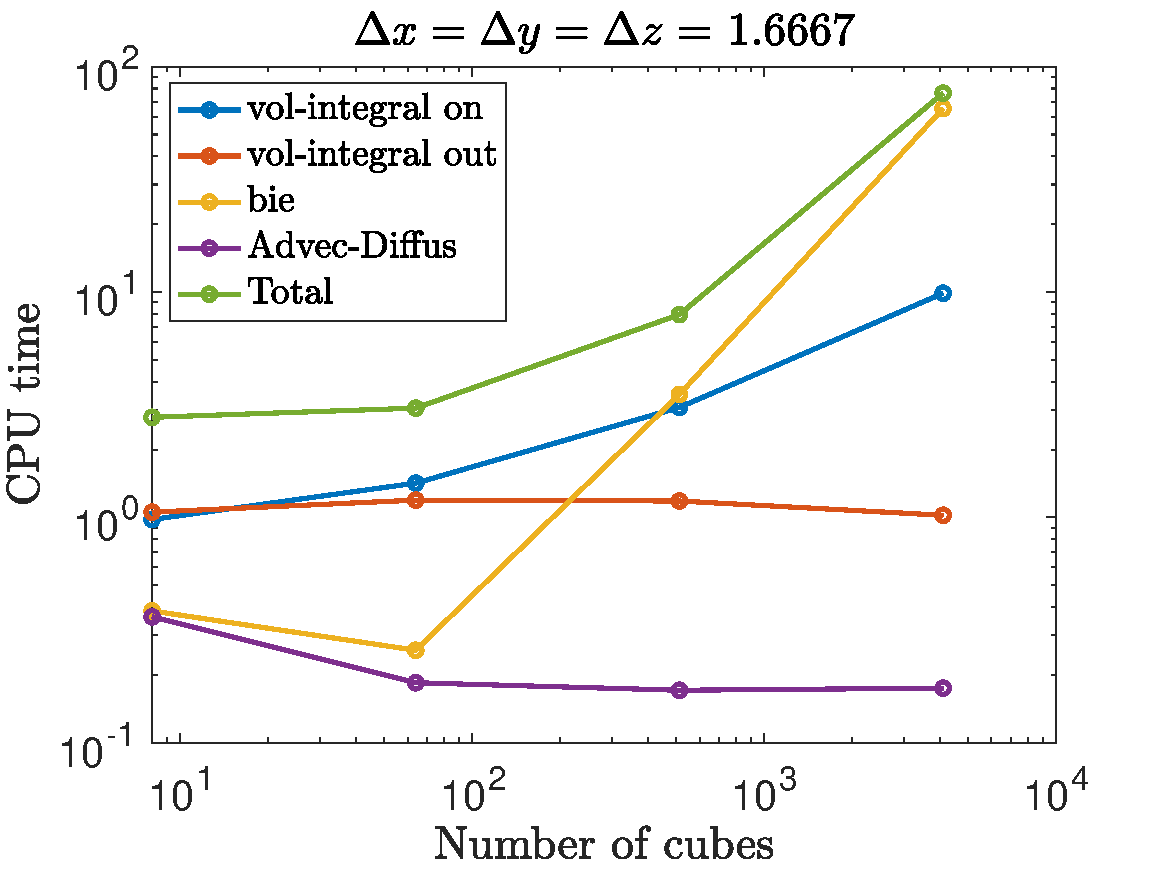
\includegraphics[scale=0.5]{./figures/fig_test_time1_fixNx}
	
	\caption{Fixed fluid domain size.}
	\label{fig_test_time1_fixNx}
\end{center}
\end{figure}

\begin{figure}[h]
	\begin{center}
		\vspace{0.5cm}
		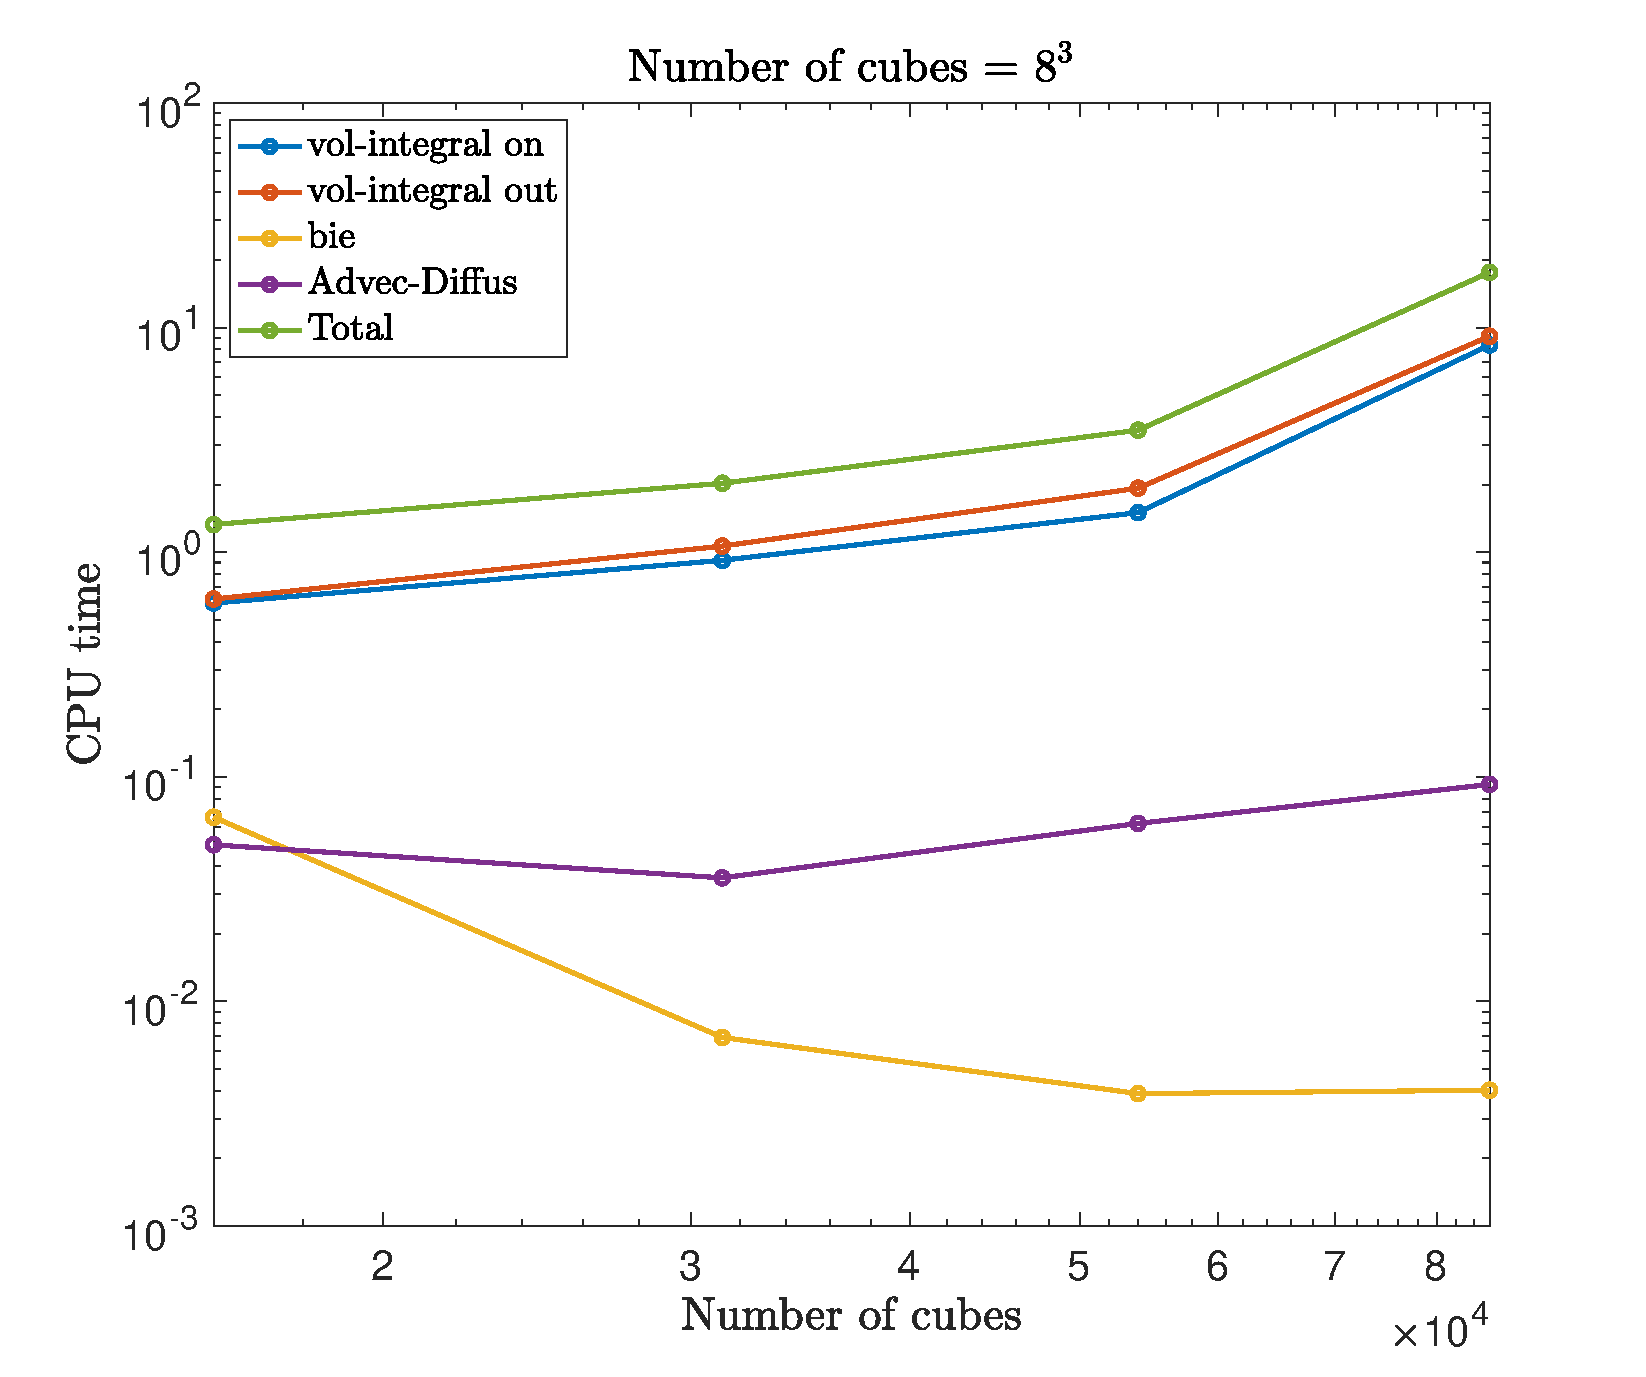
\includegraphics[scale=0.35]{./figures/fig_test_time1_varNx}
	
	\caption{Fixed aggregate size; Wrong labels. Number of cubes is $8$ and $x$-axis represents the number of total grid points. }
	\label{fig_test_time1_varNx}
\end{center}
\end{figure}

\clearpage
Today is 09/06/2022. We ran 10 time-steps for each case. The following is the setting I used to check the runtime. 
\begin{framed}
	\begin{itemize}
		\item Reference length scale: $L = 5 \times 10^{-4}$(m).
		\item Gravitational acceleration $g = 9.8$ (m$/$s$^2$).
		\item $\mu = 1.2 \times 10^{-3}$ (kg$/$ ms) .
		\item $\rho_s = 1.4 \times 10^{3}$ (kg$/$ m$^3$) .
		\item $\rho_0 = 1.025 \times 10^{3}$ (kg$/$ m$^3$) .
		\item $\phi = 0.9999$
		\item $\gamma = -10^{-5}$.
		\item $\alpha = 1$.
		\item $C(\vec{x}, 0) = 0$ (everywhere).
		\item Peclet number = 50.
		\\
		\item \verb+Nx = [2^3, 2^4, 2^5, 2^6]+
		\item \verb+Ny = Nx, Nz = 2Nx+
		\item Fluid domain size: $[-20, 20] \times [-20, 20] \times [-40, 40]$
		\item \verb+dt = 0.1+
		\item \verb+Nt = 10+
		\item Rotation off 
		\item \verb+NC = 8+ (Cube shape)
	\end{itemize}
\end{framed}
\begin{figure}[h]
	\begin{center}
		\vspace{0.5cm}
		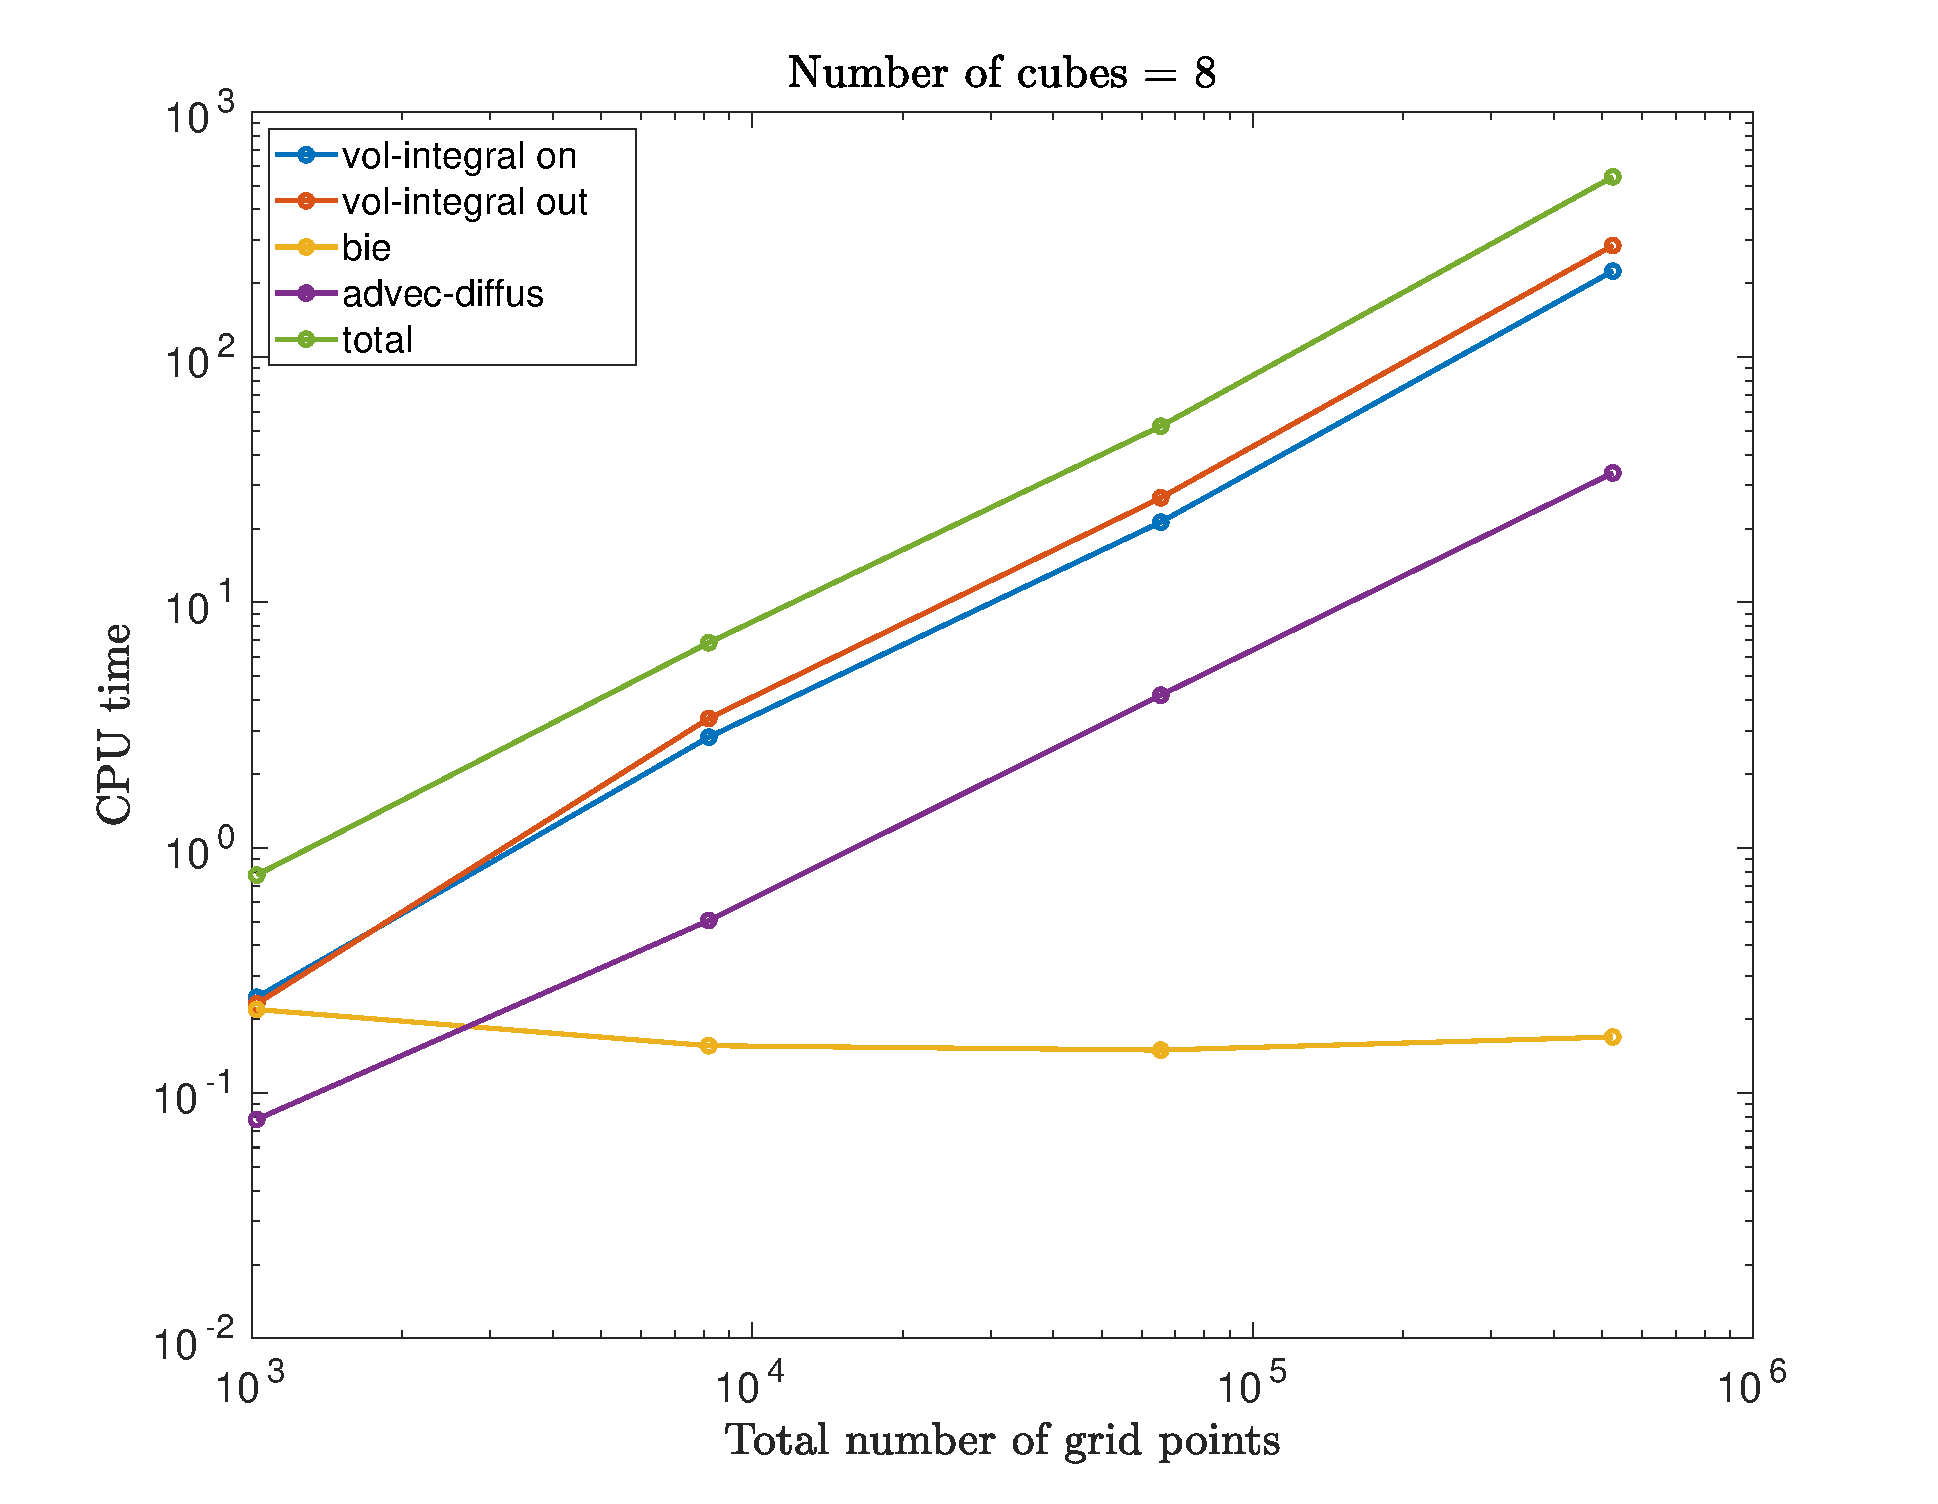
\includegraphics[scale=0.3]{./figures/fig_10time_NC8_varNx}
	
	\caption{Number of cubes is 8. }
	\label{fig_10time_NC8_varNx}
\end{center}
\end{figure}
%
% \begin{figure}[h]
% 	\begin{center}
% 		\vspace{0.5cm}
% 		\includegraphics[scale=0.33]{./figures/fig_10time_NC125_varNx}
% 		\includegraphics[scale=0.33]{./figures/fig_vel_test2-2}
	
% 	\caption{Number of cubes is 125. }
% 	\label{fig_10time_NC125_varNx}
% \end{center}
% \end{figure}
\clearpage
[Updated on 01/26/2023]
%
% \begin{figure}[h]
% 	\begin{center}
% 		\vspace{0.5cm}
% 		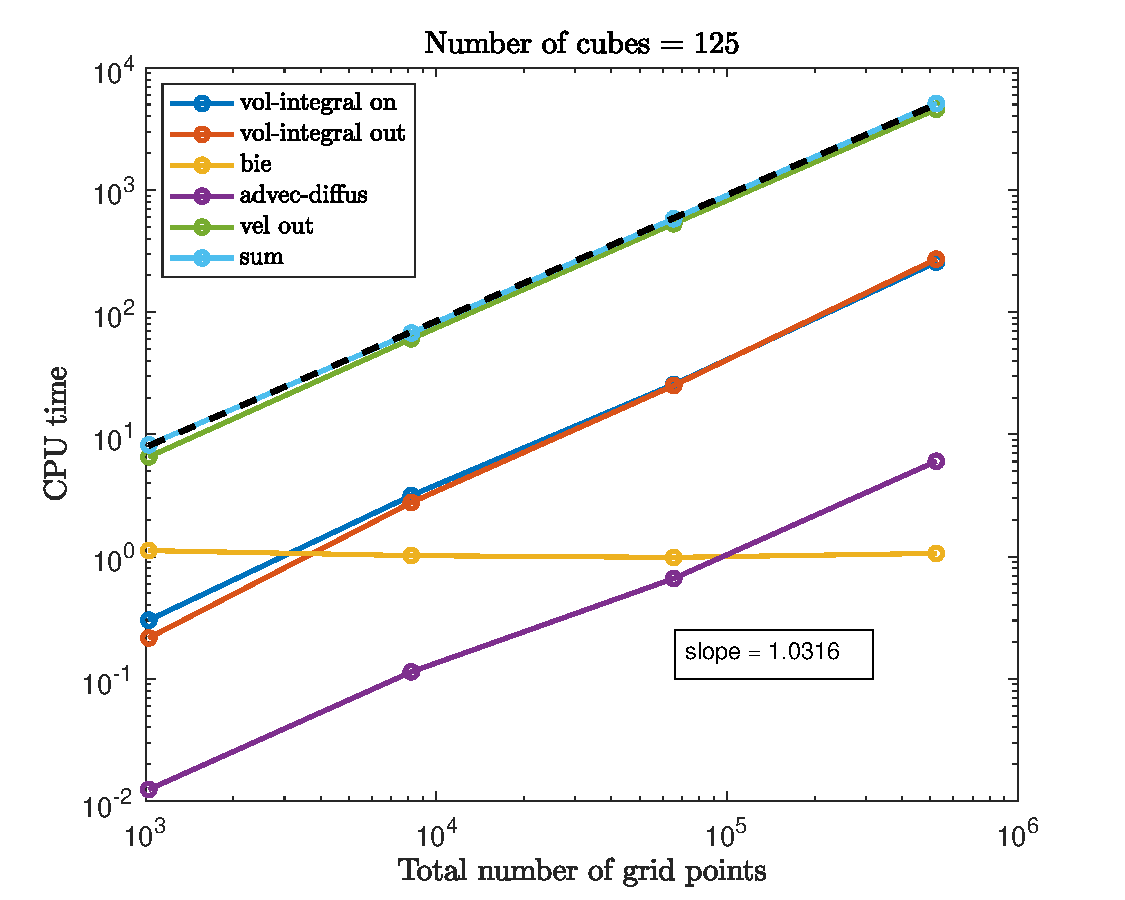
\includegraphics[scale=0.5]{./figures/fig_time_varNx5}	
% 	\caption{Number of cubes is 125.}
% 	\label{fig_time_varNx5}
% \end{center}
% \end{figure}
\begin{figure}[h]
	\begin{center}
		\vspace{0.5cm}
		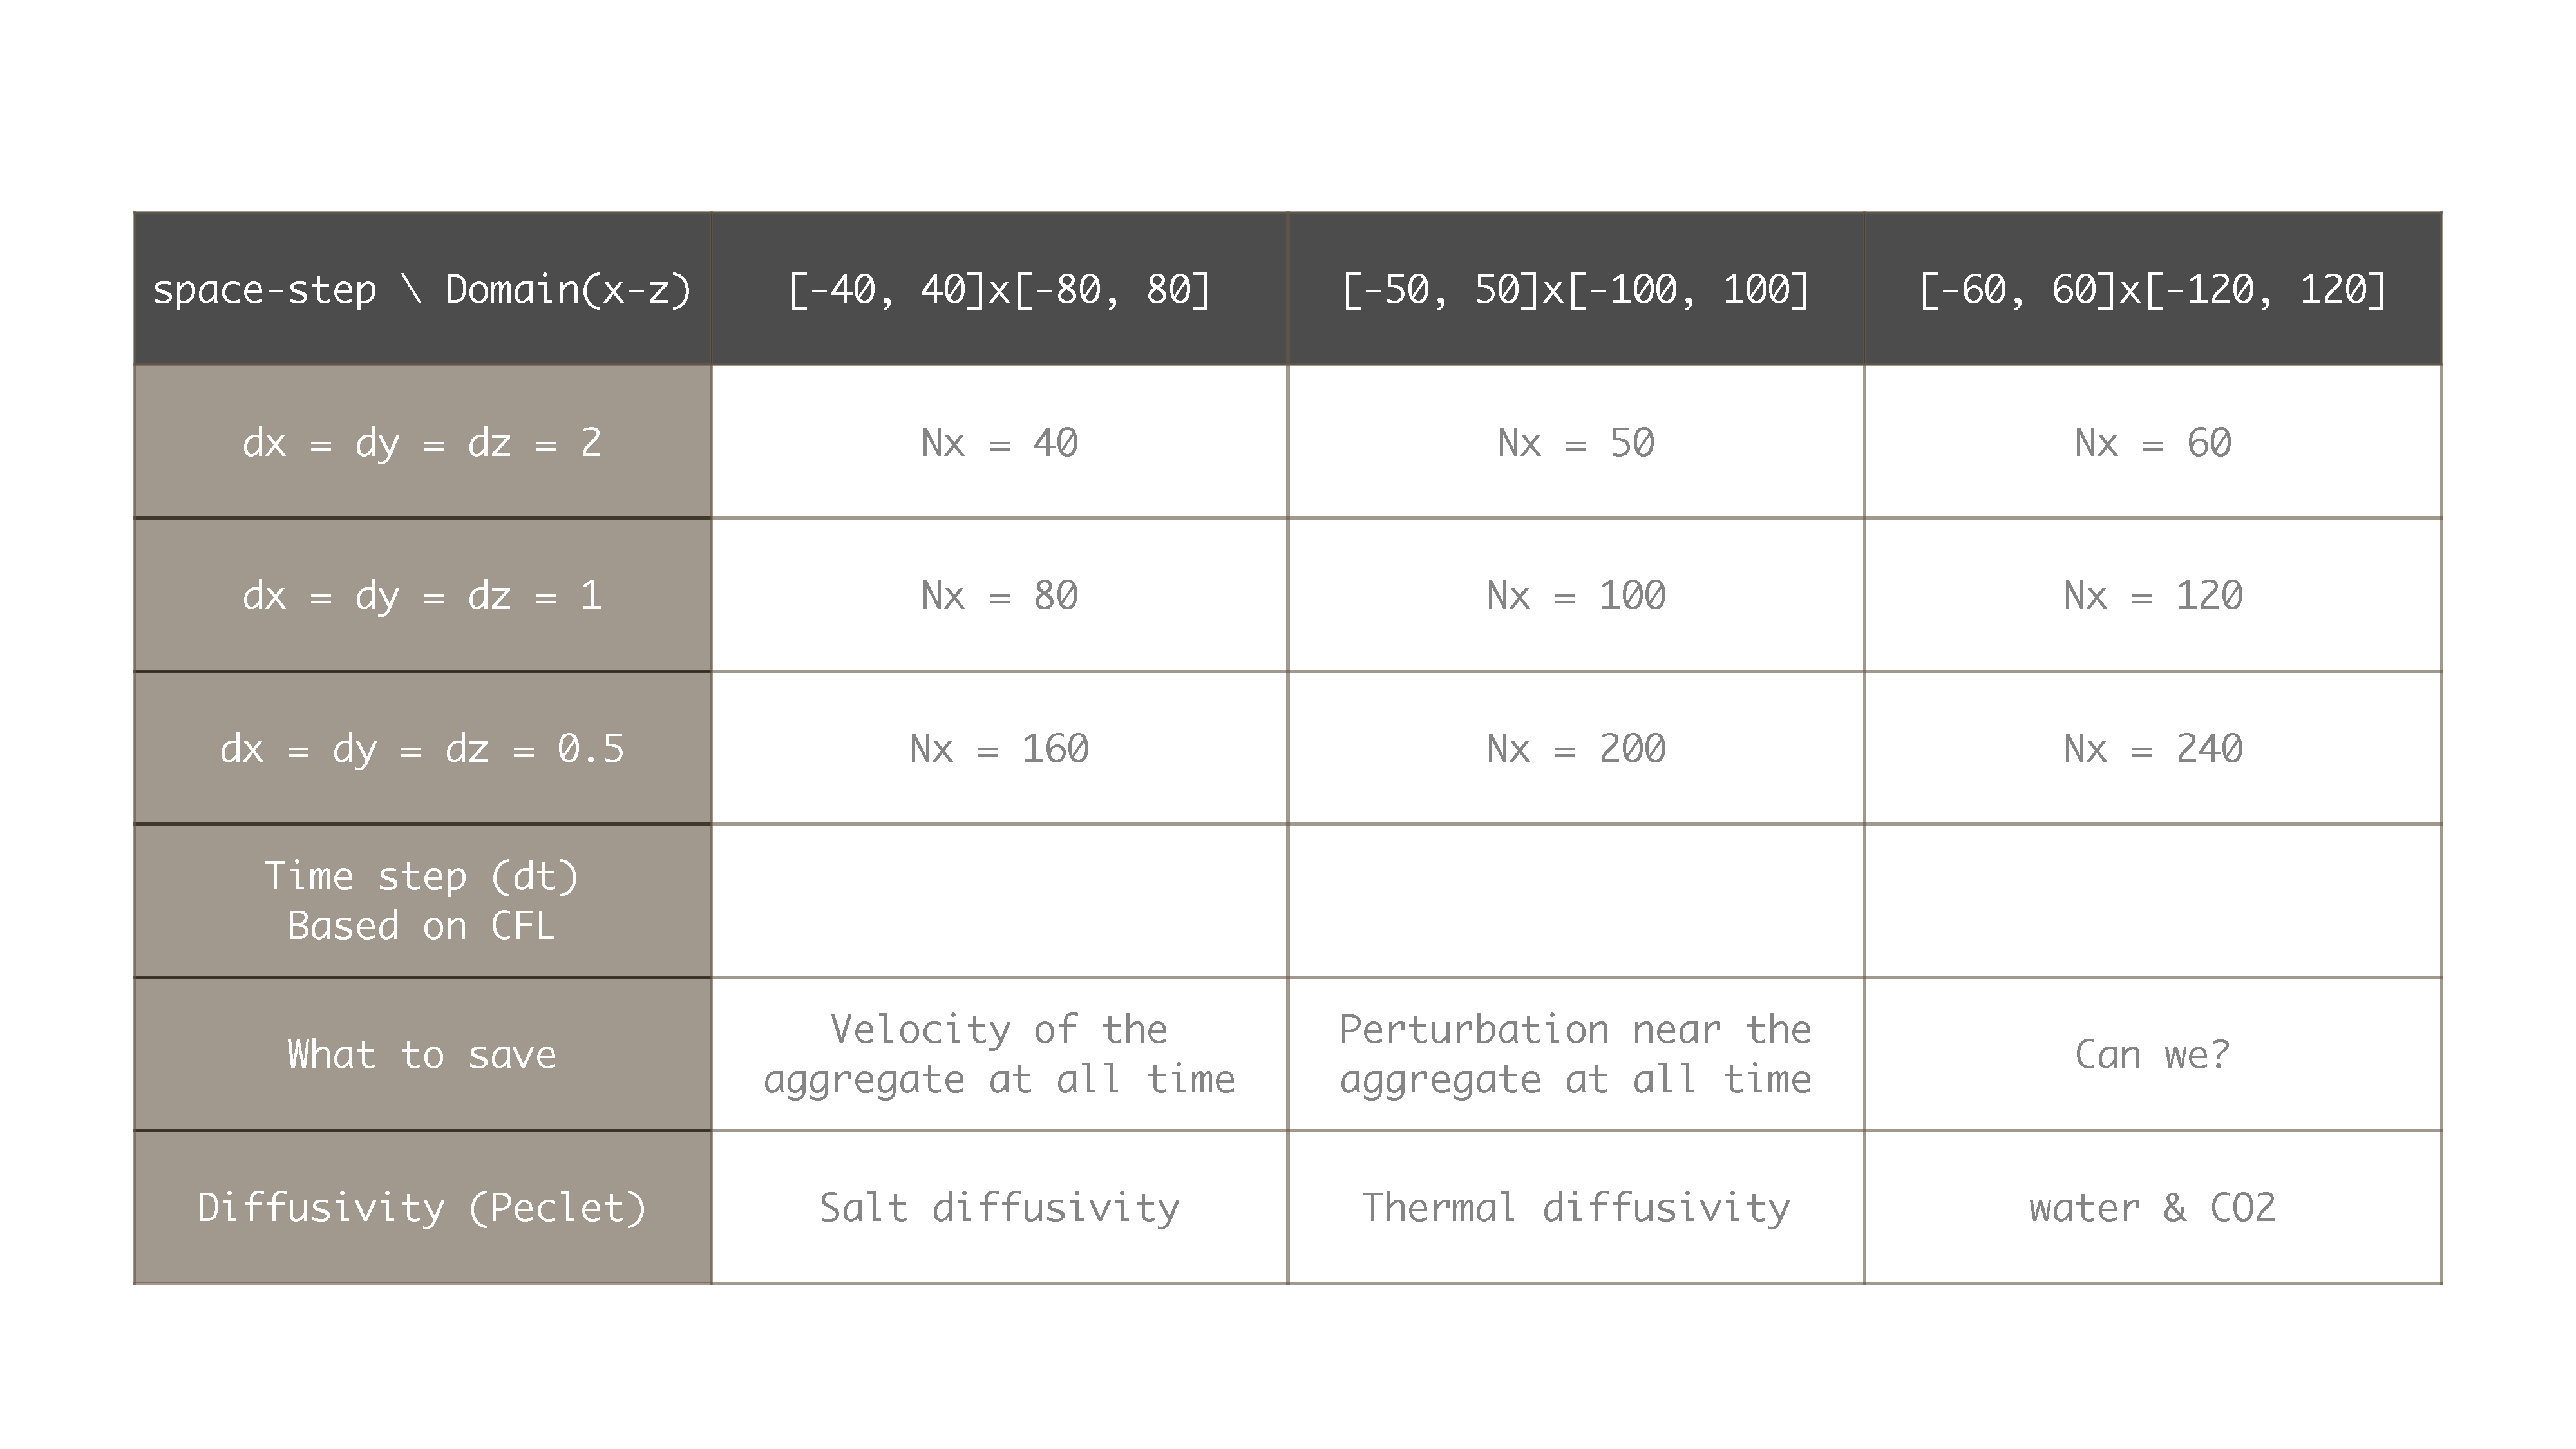
\includegraphics[scale=0.25]{./figures/table_agg_MERCED}	
	\caption{What we should run.}
	\label{fig_map_MERCED}
\end{center}
\end{figure}
\\
How can we determine the time-step size, $\Delta t$? We need to consider CFL here, for both advection and diffusion. 
\\
Knowing that the unit of diffusivity is [D] = $L^2/T$, we consider 
\[
R_{max}^2 \sim \text{Pe} \Delta t,
\]
wherer $R_{max}$ is a maximum radius of the aggregate. 
\end{comment}
\subsection{Homogeneous velocity computation with FMM}
We noticed that the homogeneous velocity computation using the boundary integral equation is quite slow, due to the large number of fluid domain grid points. We thus attempt to use the fast multipole method (FMM) for this surface integral, by approximating as following:
\begin{equation}
	u_H(\vec{y})  
	= \int_S \vec{f}(\vec{x}) \cdot \bar{\bar{G \ }}( \vec{x}, \vec{y}) \ \text{d} S(\vec{x}),
	\label{eq_uH}
\end{equation}
where $\vec{y}$ is points in the fluids, outside of the aggregate boudnary. Note that we call $\vec{x}$ as source, since they are on the integral domain, and $\vec{y}$ as target point. 
For the velocity inside and on the aggregate boundary, we use the rigid boundary velocity $u(\vec{x}) = \vec{U}_a + \vec{\Omega} \times \left(\vec{x} - \vec{x}_{cm} \right)$. This implies that we do not expect any singularity in this computation ($\vec{x} \neq \vec{y}$), however, we may have close evaluation problem. We will discuss the size of error in the next section. 
% Let $r_{nm} = \|\vec{x}^n - \vec{y}^m \|$. 
\par
Using the Laplace kernel, we can re-write the surface integral (\ref{eq_uH}) as
\begin{equation}
	u_H(\vec{y}) =
	\int_S 
	\vec{f}(\vec{x}) \cdot
  	\left(
  	\frac{\bar{\bar{I \ }}}{\|\vec{x} - \vec{y}\|}
  	- \left( \vec{x} - \vec{y} \right)
  	 \nabla_{\vec{x}}
  	\frac{1}{\|\vec{x} - \vec{y}\|}
  	\right)
	  \ \text{d} S(\vec{x}).
 \label{eq_surf_laplace}
\end{equation}
We first discretize the entire aggregate surface into $Nf$ number of square faces that are located at $[cx_1^n-1, cx^n_1+1] \times [cx^n_2-1, cx^n_2+1]$. This refers that $(cx^n_1, cx^n_2)$ is the center of $n-$th square face. The discretized version of the velocity equation (\ref{eq_surf_laplace}) is denoted by $H(\vec{y})$,
\begin{align}
	H(\vec{y}^m) & = u_H(\vec{y}) - E_f
	 = \sum_{n = 1}^{Nf} H^n(\vec{y}^m) 
	\nonumber \\
	& = \sum_{n = 1}^{Nf} 
	\vec{f}(\vec{x}^n) \cdot
	\int_{cx^n_2-1}^{cx^n_2+1} \int_{cx_1^n-1}^{cx_1^n+1}
  	\left(
  	\frac{\bar{\bar{I \ }}}{\|\vec{x}^n - \vec{y}^m\|}
  	- \left( \vec{x}^n - \vec{y}^m \right)
  	 \nabla_{\vec{x}^n}
  	\frac{1}{\|\vec{x}^n - \vec{y}^m\|}
  	\right)
	  \text{d} x_1  \text{d} x_2
	  ,
 \label{eq_surf_fmm_Nf}
\end{align}
where $m = 1, \  2, \cdots, \ M$, and $M$ is the total number of targets (where we want to obtain the velocity).  Note that the stress $\vec{f}(\vec{x}^n)$ is assumed to be constant over each square face. The error coming from this approximation is denoted as $E_f$; its error analysis is discussed in our previous paper \cite{yoo_hydrodynamic_2020}. One can find that we have the largest error at the corner of the cube. We would like to keep this true as we make further approximation. 
%We may begin using the FMM3D code for each $\vec{x}^n$ for now (using the FMM3D $Nf$ times {\color{red} $\rightarrow$ This is fixed now. Total 18 times we use. how did you do it?}). We should be able to edit the code for efficiency. 
% Since we need to compute two terms inside of the itnegral separately,
\par
Next, we need to approximate the surface integral in equation (\ref{eq_surf_fmm_Nf}) using a Riemann sum,
% {\color{blue} We should perform an error analysis for this entire computation.}
% For the simplicity, we first consider the integral over one square face. 
% For each $n$, we have
\begin{align}
	\tilde{H}^n(\vec{y}^m) 
	& = H^n(\vec{y}^m) - E_{G} 
	\nonumber \\ 
	& =
	\sum_{n = 1}^{Nf} 
	\vec{f}(\vec{x}^n) \cdot
	\sum_{s=1}^{Ns^2} d^2 
  	\left(
  	\frac{\bar{\bar{I \ }}}{\|\vec{x}_s^n - \vec{y}_s^m\|}
  	- \left( \vec{x}_s^n - \vec{y}^m \right)
  	 \nabla_{\vec{x}_s^n}
  	\frac{1}{\|\vec{x}_s^n - \vec{y}^m\|}
  	\right)
	  + E_{G},
 \label{eq_surf_fmm_Nf_n}
\end{align}
where $E_G$ is the error coming from the quadrature method. 
We make $Ns$ number of sub-squares, that have sizes of $d = 2/Ns$, and take the center of each sub-squares as the integration points. 
We take the same number of points, $Ns$, evenly distributed, in one direction. We can also consider the number points as the number of sub-squares in one face. 
In the following schematics, Figurue \ref{fig_face_grid}, the red cross represents the center of the $n-$th square face, $(cx^n_1, cx^n_2)$.
\begin{figure}[h]
	\begin{center}
		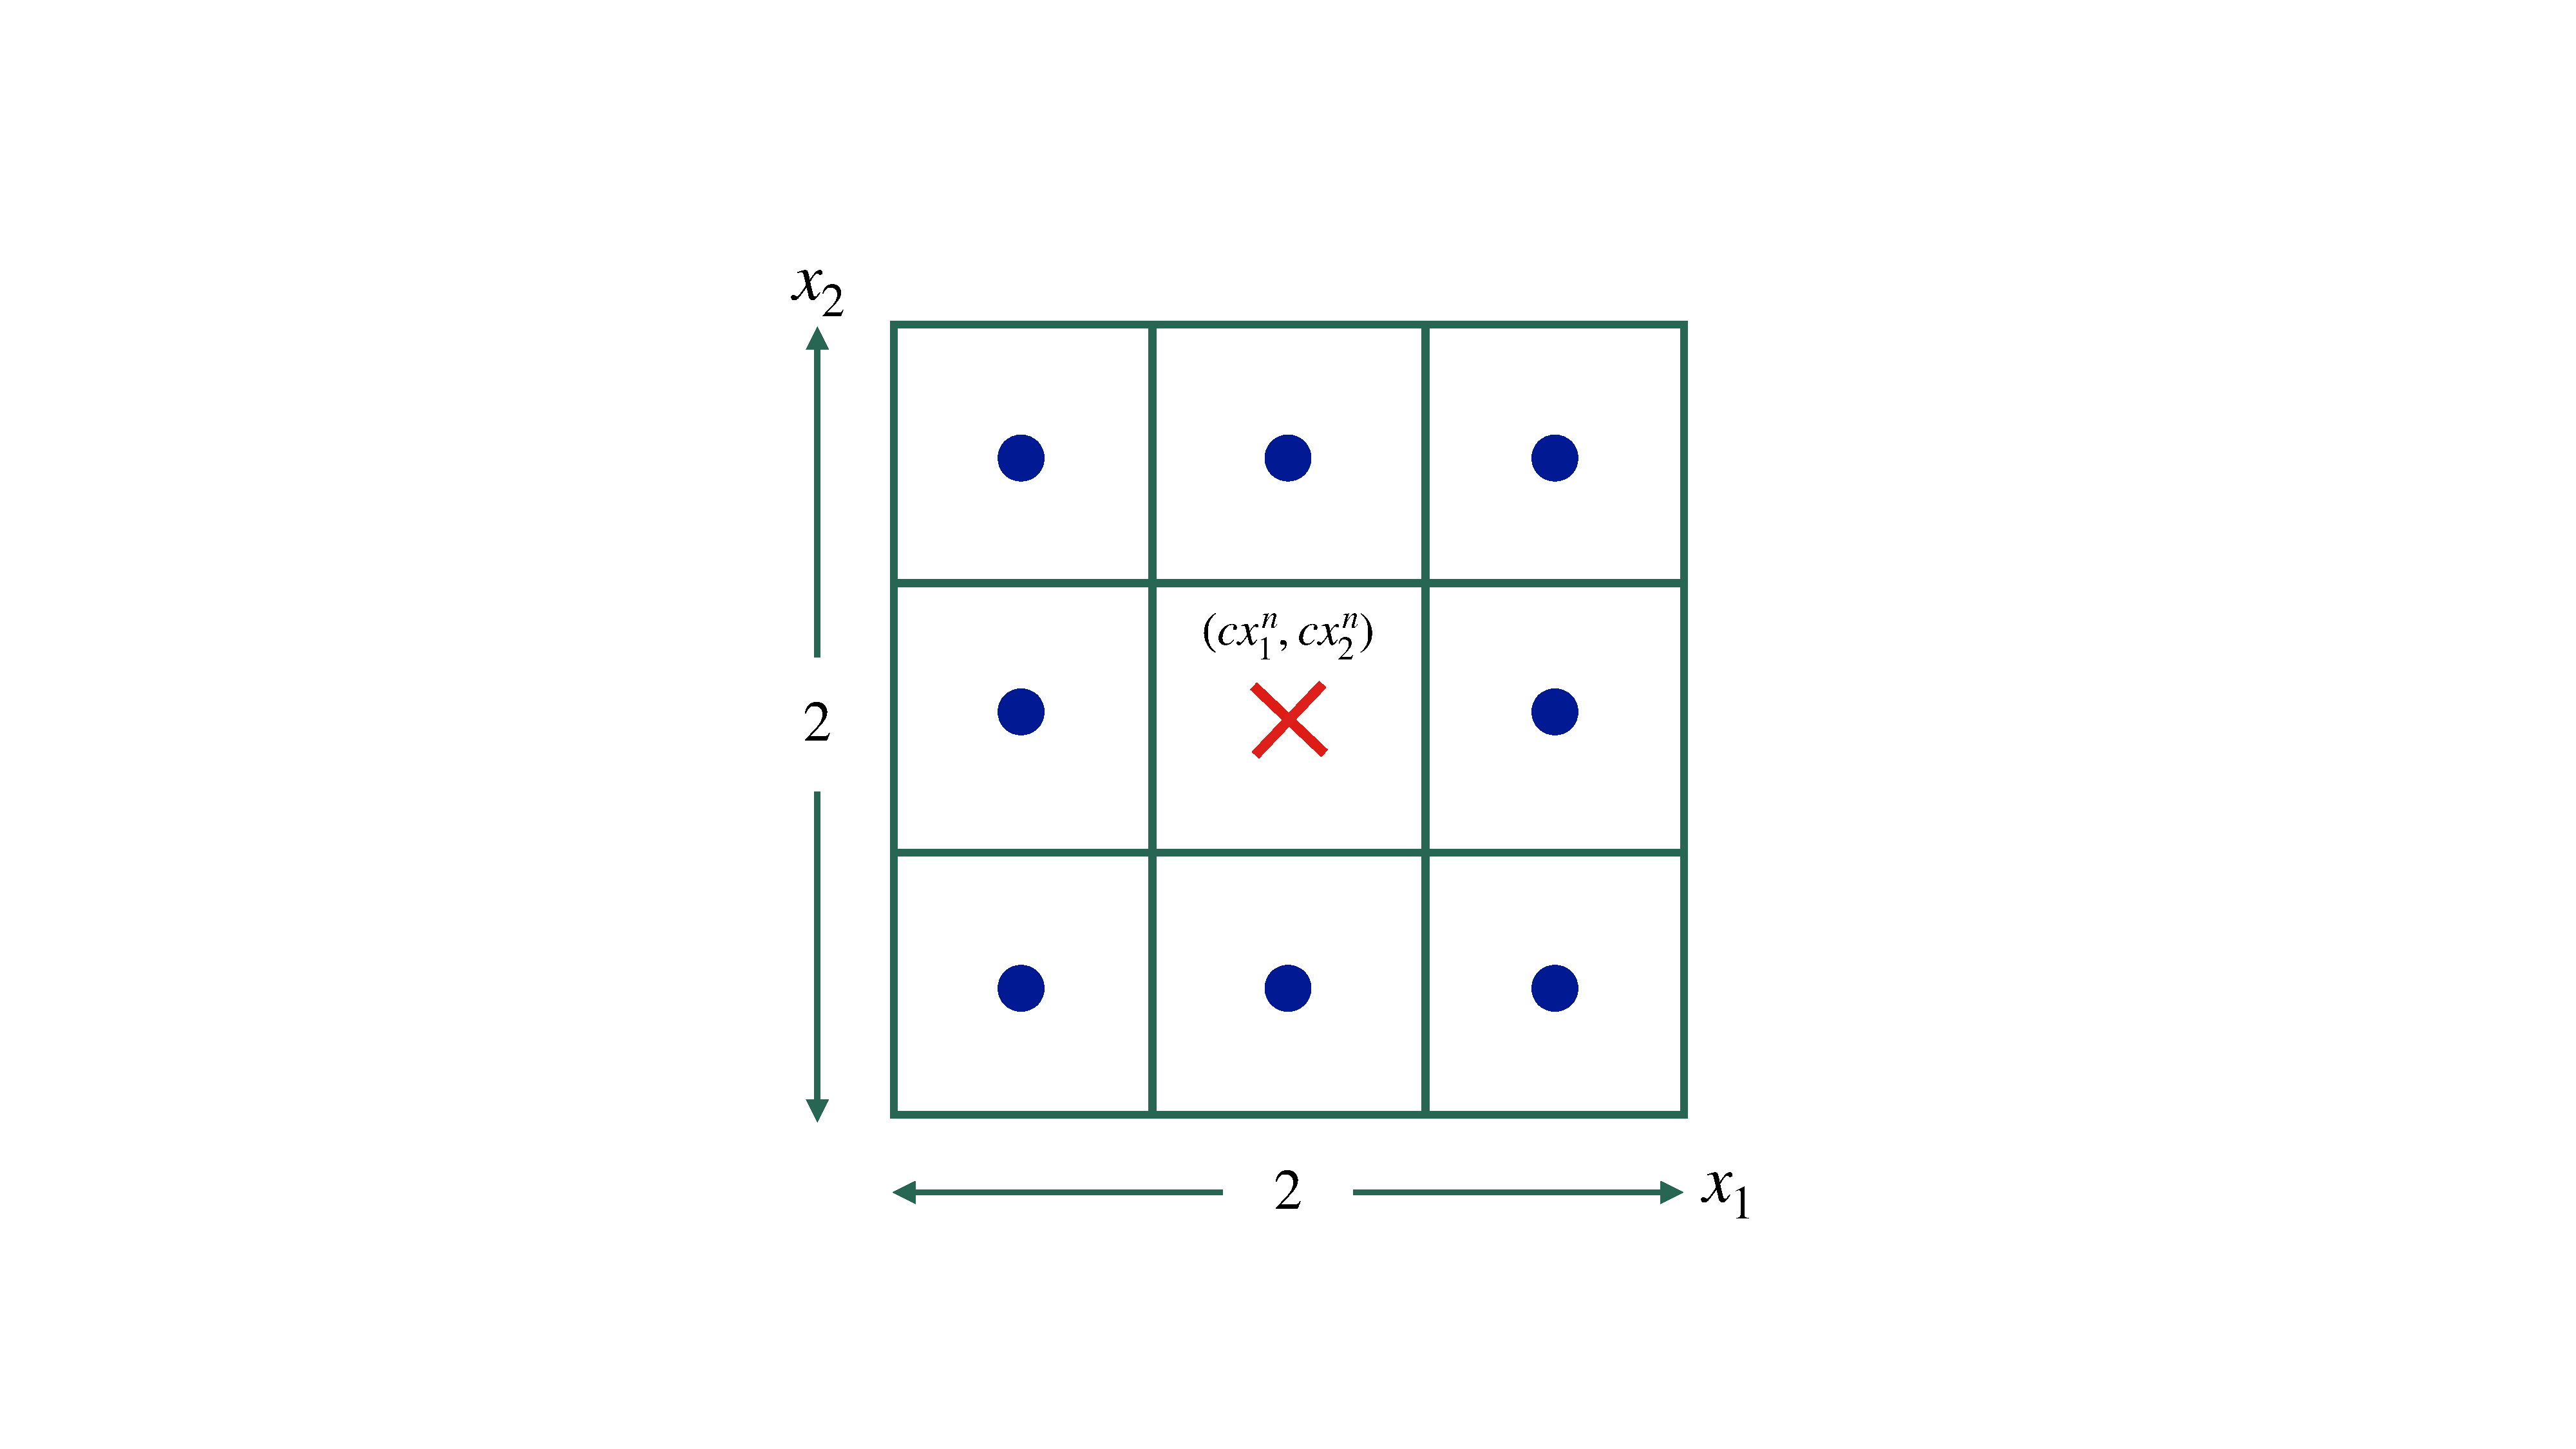
\includegraphics[scale=0.17]{./figures/fig_face_grid}
	\caption{Schematic of points we use to approximate the integral of the single-layer potential kernel over one square face.}
	\label{fig_face_grid}
\end{center}
\end{figure}
Including the center, that is the red cross, the blue dots are the integration points.
% For the horizontal, $x_1$-direction, we create an array as \verb+x1 = -floor(Ns/2):floor(Ns/2)+, and the  coordinates of those points are \verb+x1Span = cx1 + d.* x1+
For simplicity, we may not include any boundary values on one square face.
\par
% \subsection{Error analysis}
As we mentioned, we hope to have a reasonable size of the integration error, $E_G \ll E_f$.
In order to measure $E_f$, we consider the settling of one cube shape aggregate.
We then observe the relative error of the vertical velocity on one square face, considering the translational velocity, $\vec{U}_a$, as the exact solution. Note that we do not have rotation, i.e., $\vec{\Omega} = \vec{0}$. 
\begin{figure}[h]
	\begin{center}
		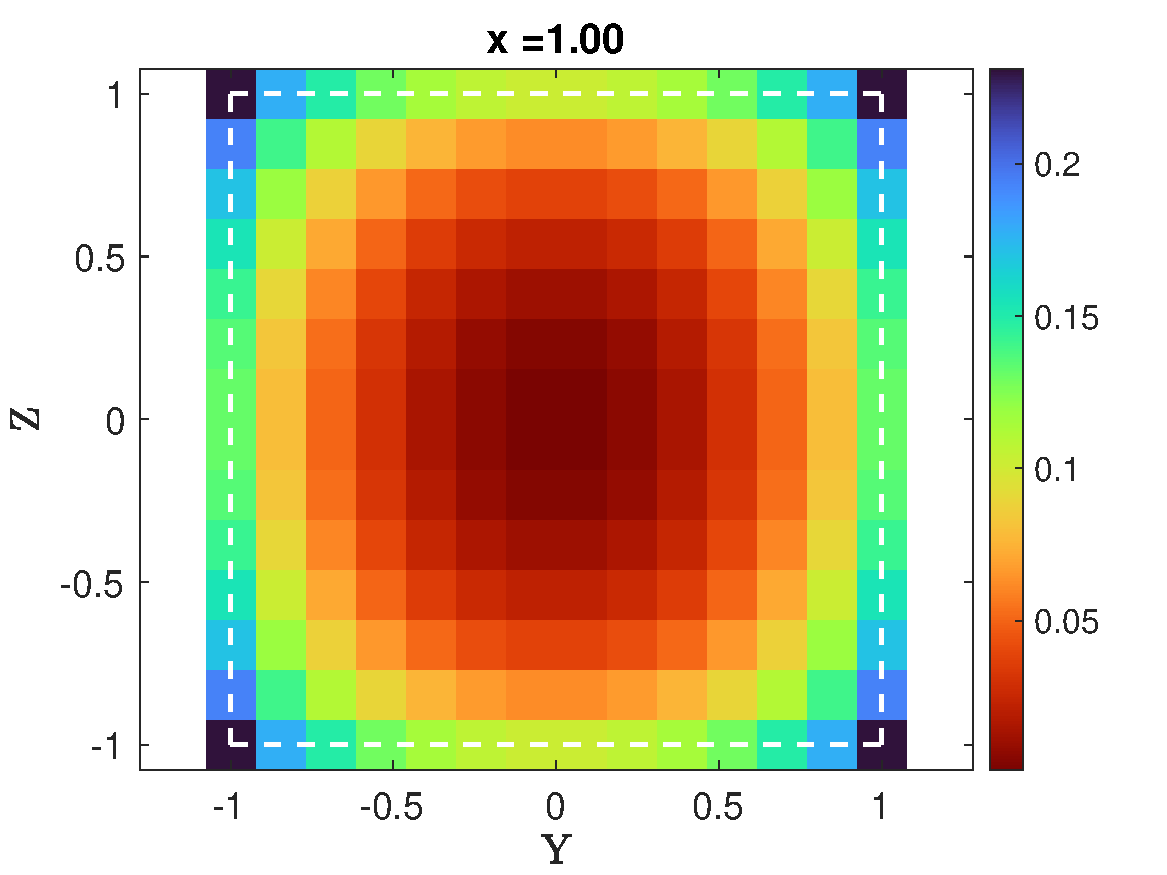
\includegraphics[scale=0.3]{./figures/fig_corner_err}
	\caption{Relative error of }
	\label{fig_corner_err}
\end{center}
\end{figure}
In figure \ref{fig_corner_err}, we see the square face at $x = 1.00$, where the white dashed line shows the location of the square face, and the color shows the relative error. It implies that the maximum of 23.12$\%$ error occurs at the corner of the cube, as we expected. We thus would like to regulate the quadrature error, $E_G$, accordingly by adjusting the total number of integration points, $Ns^2$.
\par
{\bf To clarify what we want to do:}
Let $u_H(\vec{y})  = U = F \cdot  G$ be the exact or true velocity computation. Then 
\begin{align}
	U^* = F^* \cdot  G
	\\
	U^{*+} = F^* \cdot  G^+
\end{align}
where $F = F^* + E_f$ and $G =  G^+ + E_G$.
By approximating the integral of the kernal, using FMM3D, we compute $U^{*+}$, that is,
\begin{align}
	U^{*+} = (F-E_f) \cdot (G - E_G) 
	% \nonumber \\
	% = F \cdot G - F \cdot E_G - G \cdot E_f 
	% + E_f \cdot E_G
	% \\
	= U +  \left| E_f \cdot G + F  \cdot E_G \right|  + \mathcal{O}(E_f E_G).
\end{align}
We know that 
\[
	|U-U^*| = |E_f \cdot G| \approx 23 \%,
	\]
and we would like to have
\[
	|F  \cdot E_G| \ll	|E_f \cdot G |
\]
Note that 
\[
	  |F \cdot E_G| = |F^* \cdot E_G + E_f \cdot E_G|
	  \approx |F^* \cdot E_G |
\]
Thus, what we need to compare is two velocity approximations,
\begin{align}
	|U^* - U^{*+}| =| F^* \cdot E_G| \ll 23 \%
	\label{eq_condition_EG}
\end{align}
We vary the number of integration points to choose an optimal value. For this experiment, we set $\varepsilon = 10^{-6}$.
\begin{figure}[ht]
	\begin{center}
		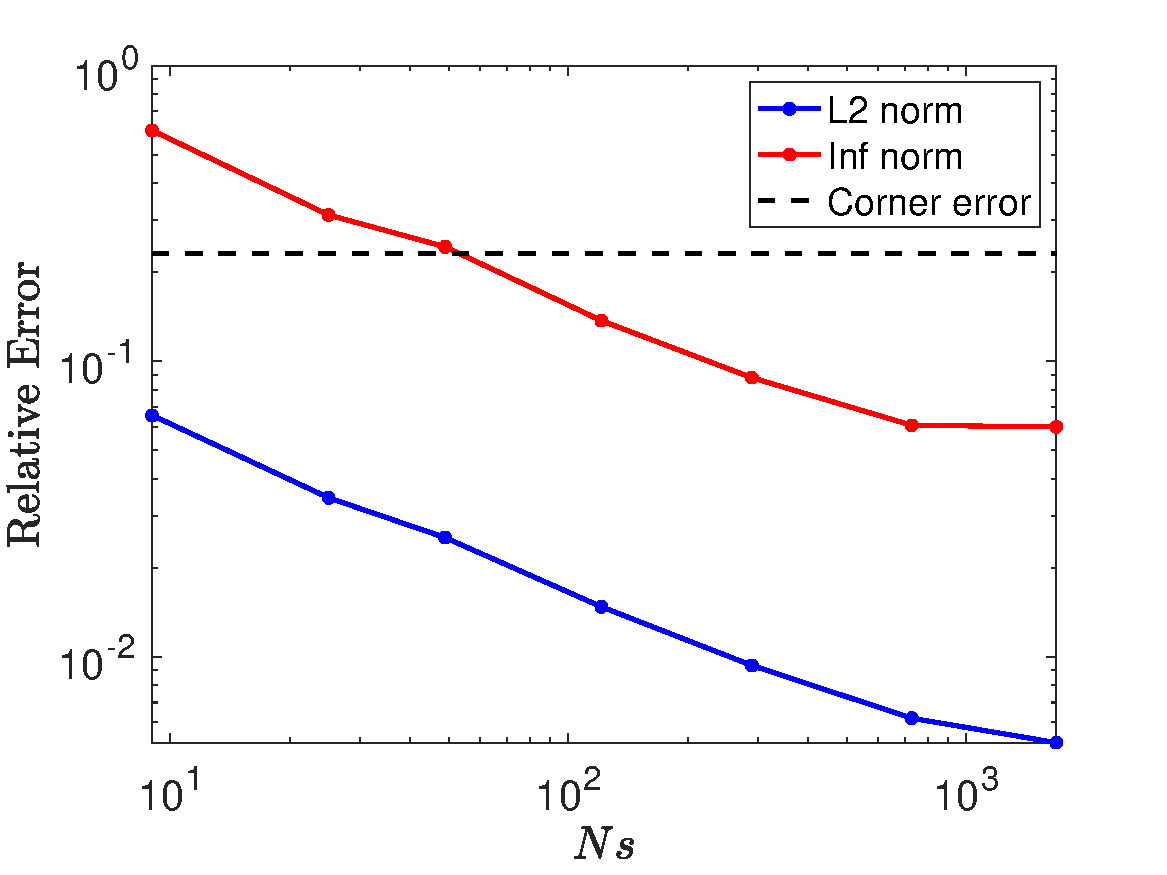
\includegraphics[scale=0.33]{./figures/fig_Ef_EG_compare}
	\caption{Relative error between $U^*$ and $U^{*+}$, varying the number of integration points: $Ns = [3, 5, 7, 11, 17, 27,41]^2$. Set $\varepsilon = 10^{-6}$.}
	\label{fig_Ef_EG_compare}
\end{center}
\end{figure}
Figure \ref{fig_Ef_EG_compare} shows that $Ns = 9^2$ points are enough to satisfy what we needed in equation (\ref{eq_condition_EG}). 
\par
When we use FMM3D library, we can choose the desired accuracy, $\varepsilon$, which determines the number of terms in the series expansion. We do not want to select too small $\varepsilon$ since it increases the computation time. Since we used $\varepsilon = 10^{-6}$ to produce figure \ref{fig_Ef_EG_compare}, we set $\varepsilon = 10^{-1}$ to see the difference. As we can see in figure \ref{fig_Ef_Eg_ep-1}, there is no difference in accuracy with higher $\varepsilon$. The reason we guess is because the corner error, $E_f$, is dominating in our approximation and it is already larger than $10 \%$. 
\begin{figure}[ht]
	\begin{center}
		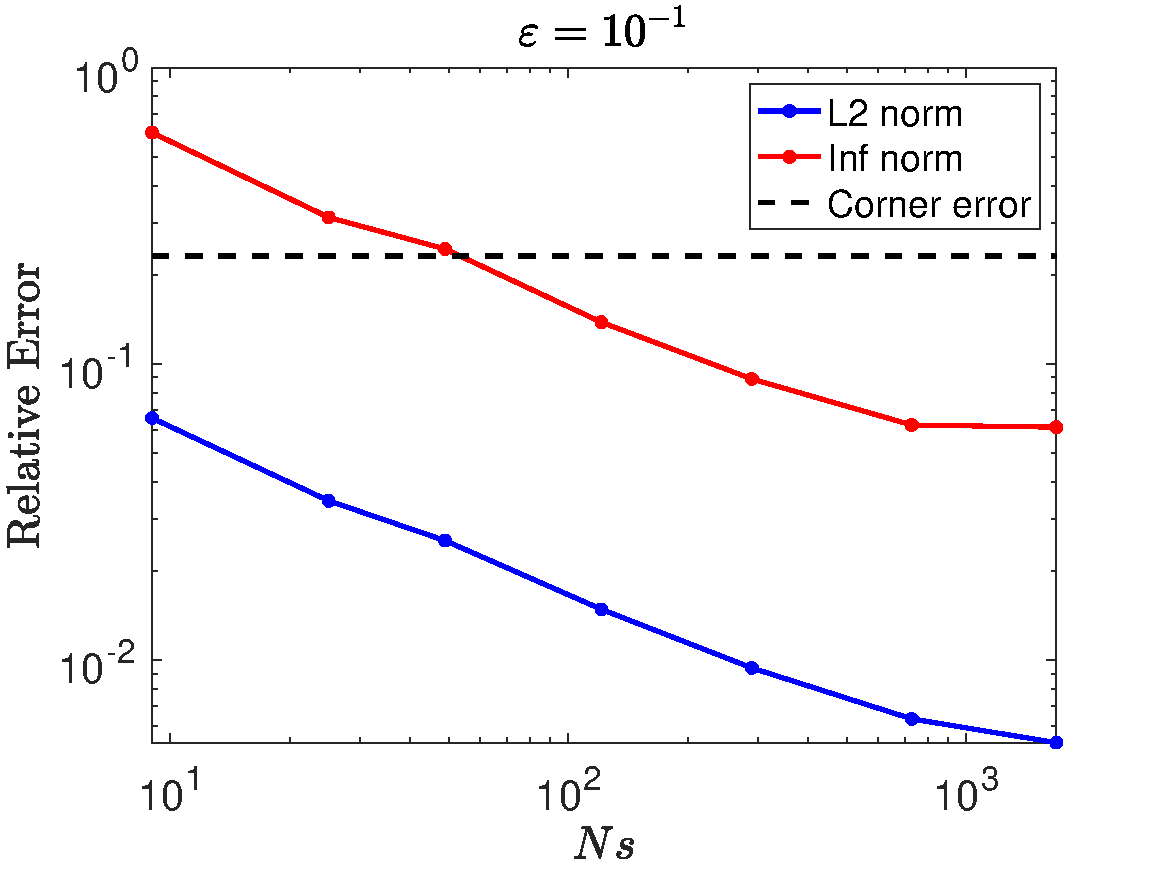
\includegraphics[scale=0.33]{./figures/fig_Ef_Eg_ep-1}
	\caption{Relative error between $U^*$ and $U^{*+}$, varying the number of integration points: $Ns = [3, 5, 7, 11, 17, 27,41]^2$. Set $\varepsilon = 10^{-1}$.}
	\label{fig_Ef_Eg_ep-1}
\end{center}
\end{figure}
In order to confirm the responses of $\varepsilon$ values, we test one-time step simulation with a smaller domain size with one cube aggregate model. Here are the exact paramesters we use:
\begin{framed}
	\begin{itemize}
		\item $\varepsilon = [10^{-1}, \ 10^{-2}, \ 10^{-3}, \ 10^{-4}, \ 10^{-5}]$
		\item \verb+Nx = 41+ ($\Delta x = 0.25$)
		\item \verb+Ny = Nx, Nz = 2Nx+ 
		\item Fluid domain size: $[-5, 5] \times [-5, 5] \times [-10, 10]$
		\item \verb+Nt = 1+
		\item \verb+NC = 1+ (Cube shape)
		\item No perturbation
	\end{itemize}
\end{framed}
Here are some results. We look at the velocity field at $x = 1.125$, that is slightly outside of the aggregate. On the right, we make a slice at $z = 0$ and see the relative error considering that velocity obtained with SLP as a reference. 
\begin{figure}[ht]
	\begin{center}
		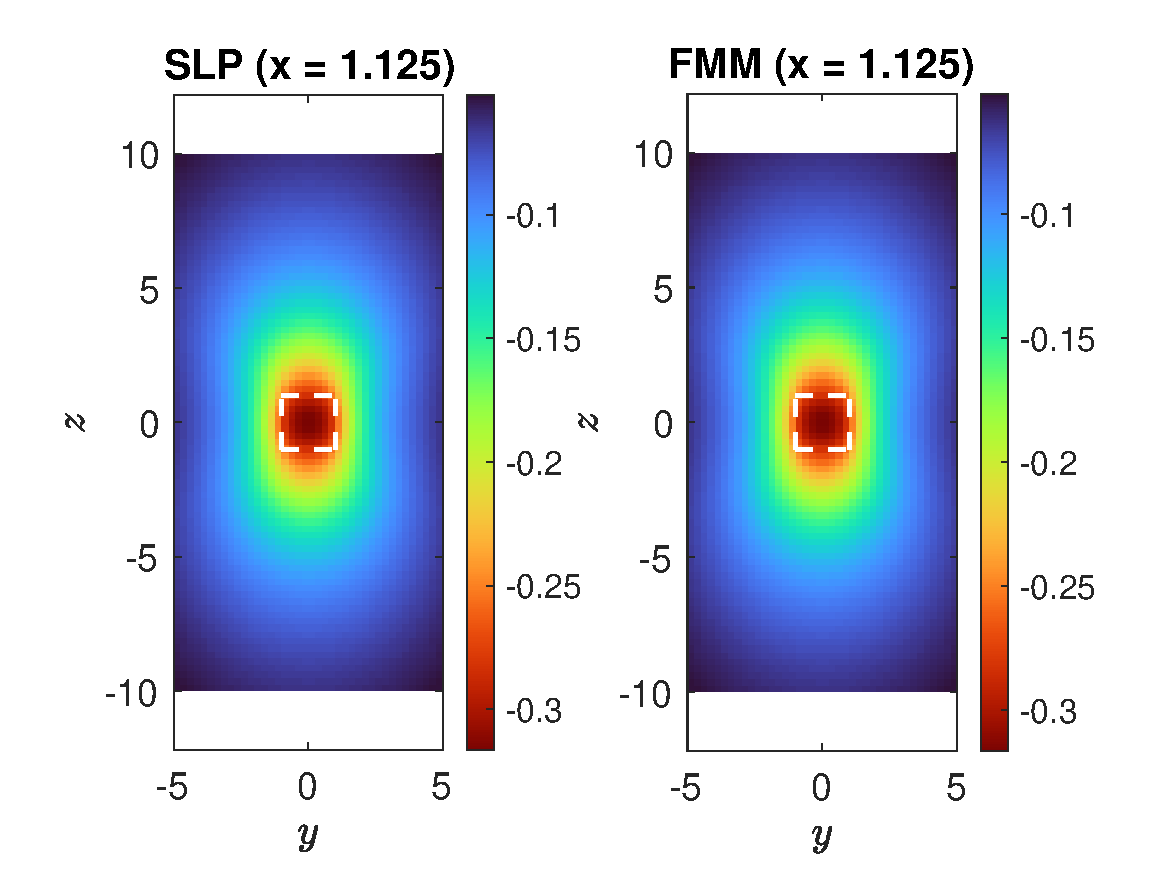
\includegraphics[scale=0.44]{./figures/fig_vel_NC1_eps1e-4}
		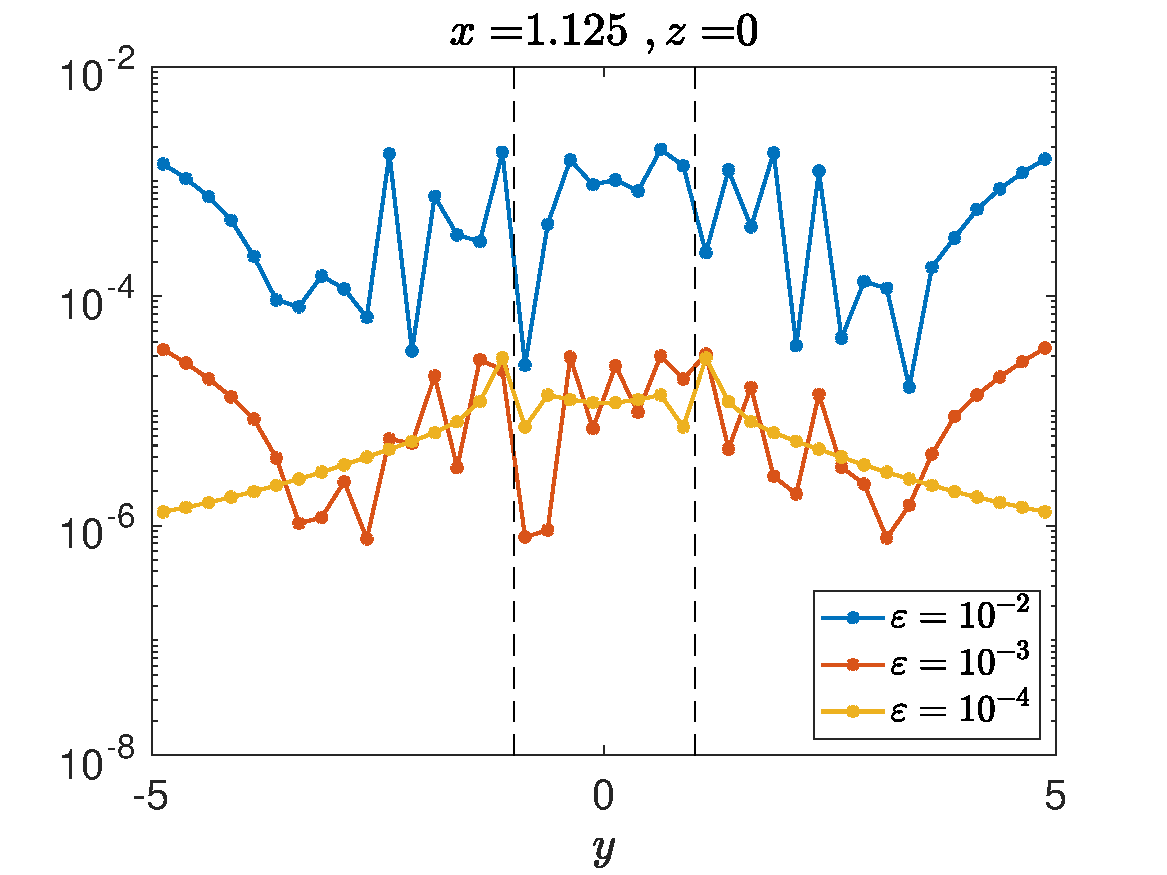
\includegraphics[scale=0.42]{./figures/fig_1Derr_NC1_eps1e-4}
	\caption{(Left) Verticle velocity field at $x = 1.125$. (Right) 1D relative error at $x = 1.125$ and $z = 0.0$ with varying $\varepsilon$.}
	\label{fig_vel_NC1_eps1e-4}
\end{center}
\end{figure}
\\
Figure \ref{fig_errNorms_varEps_NC1} shows that we may be able to obtain a good amount of error when we use $\varepsilon = 10^{-4}$. We may examine how much this choice slows the actual computation time down. 
\begin{figure}[h]
	\begin{center}
		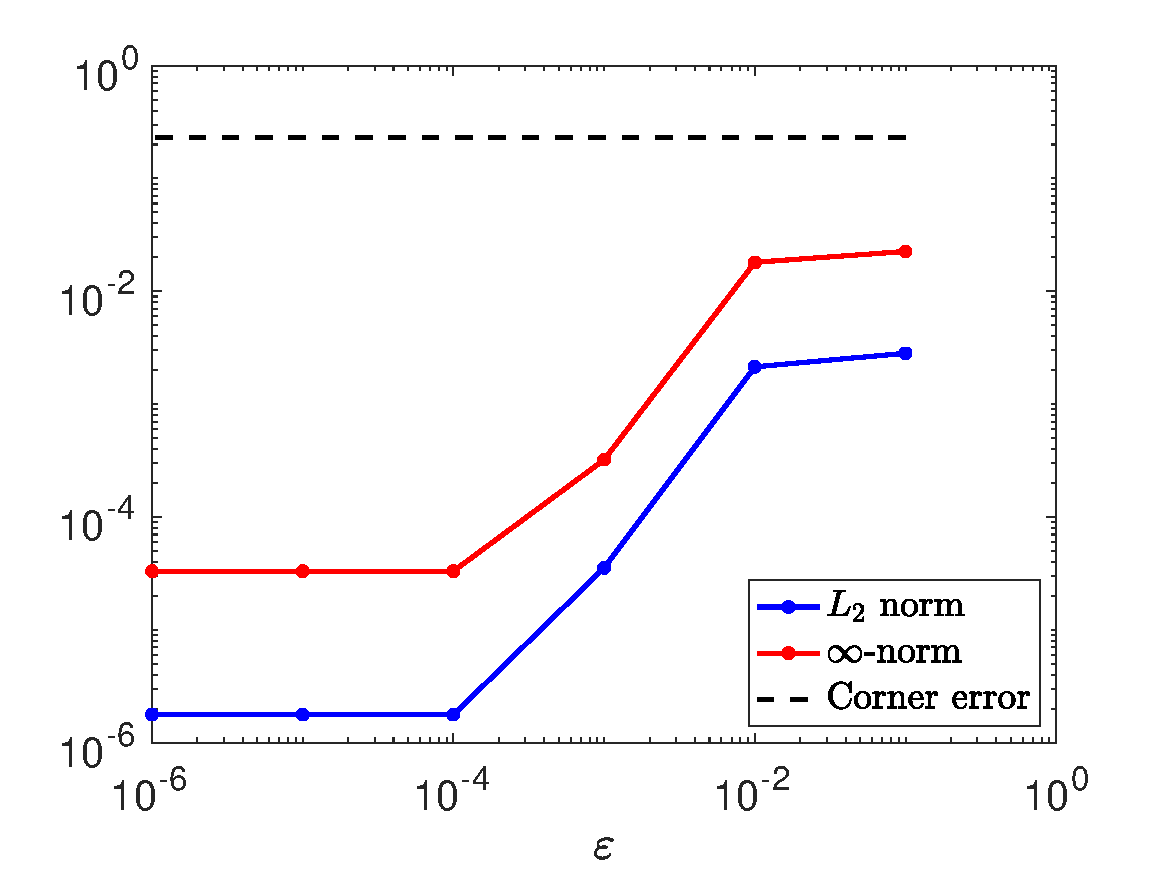
\includegraphics[scale=0.42]{./figures/fig_errNorms_varEps_NC1}
		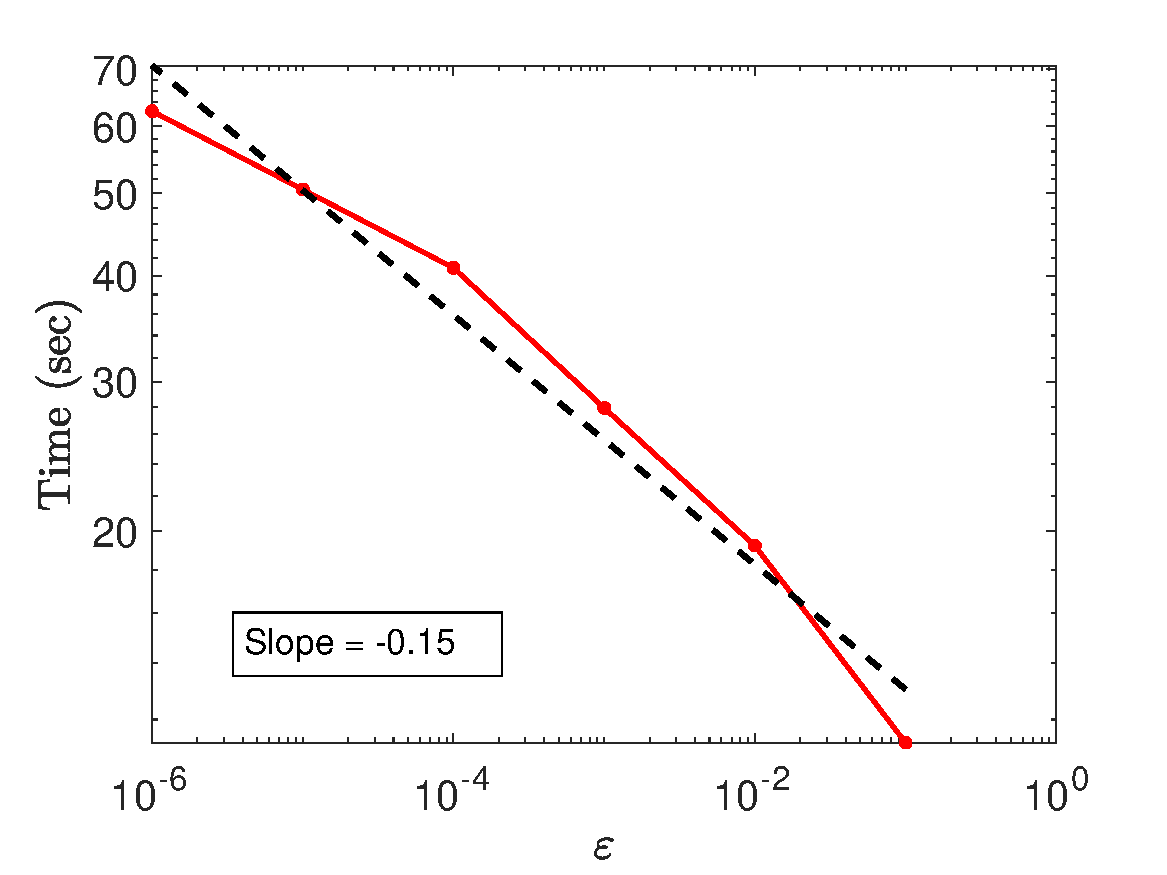
\includegraphics[scale=0.42]{./figures/fig_times_varEps_NC1}
	\caption{(Left) $L_2$ and $\infty$-norms of the velocity in the entire fluid domain. (Right) Time, in second, for one time-step computation with various $\varepsilon$.}
	\label{fig_errNorms_varEps_NC1}
\end{center}
\end{figure}
\clearpage
\subsection{Computation time results}
The data is stored in \verb+data_fmm_t10_varNx_mm5+ and the plot is generated by \verb+plot_time_varNx2+. We use the following values to compare the FMM3D computation to the previous results.
\begin{framed}
	\begin{itemize}
	\item \verb+Nx = [2^3, 2^4, 2^5, 2^6]+
	\item \verb+Ny = Nx, Nz = 2Nx+
	\item Fluid domain size: $[-20, 20] \times [-20, 20] \times [-40, 40]$
	\item \verb+dt = 0.1+
	\item \verb+Nt = 10+
	\item Pe = 50
	\item \verb+NC = 125+ (Cube shape)
	\end{itemize}
\end{framed}
The left one in figure \ref{fig_time_fmm_sum} is the previous results we observed, showing that the velocity evaluation using original SLP code is dominating the computation time. With the same setting, the right plot shows that we can reduce the time almost 10 times by applyting the FMM3D. We yet introduced the quadrature error, but make sure to be smaller than the corner error. 
\begin{figure}[ht]
	\begin{center}
		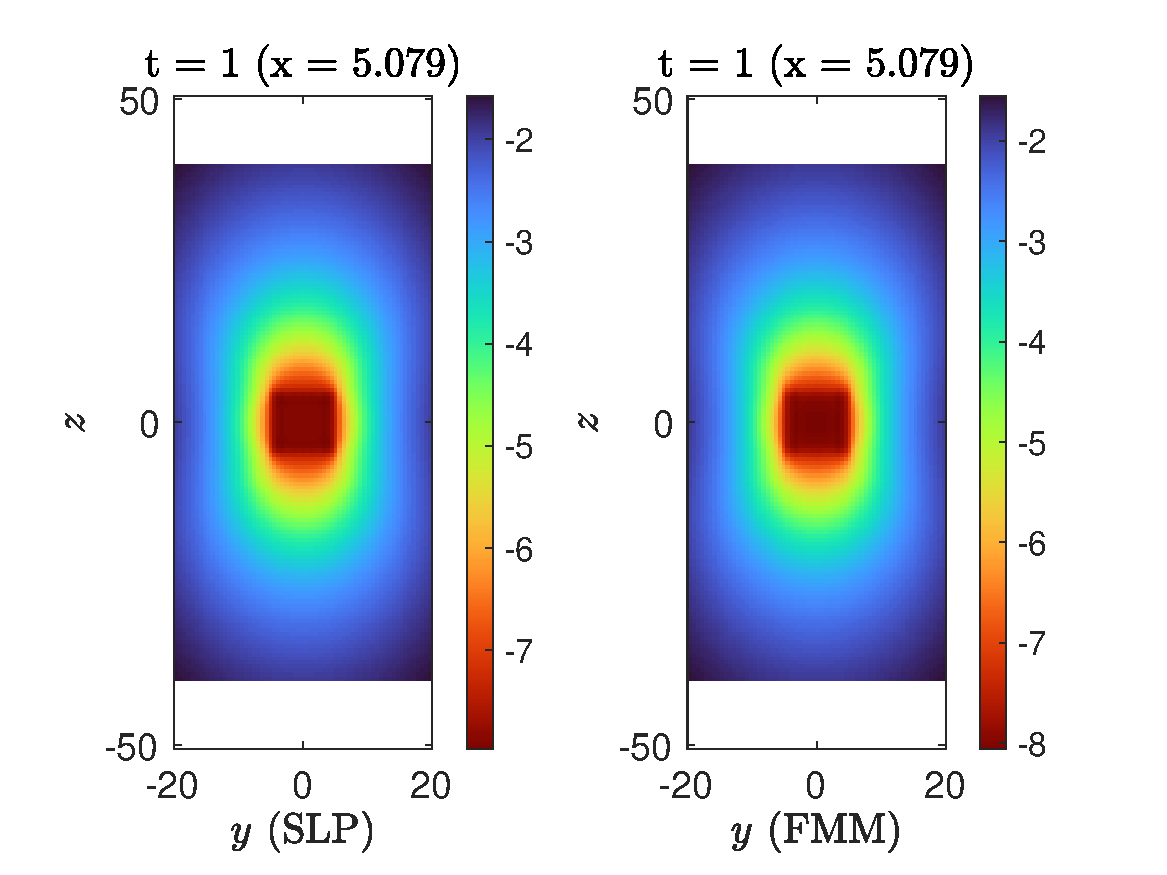
\includegraphics[scale=0.42]{./figures/fig_vel_mm5_t1}
		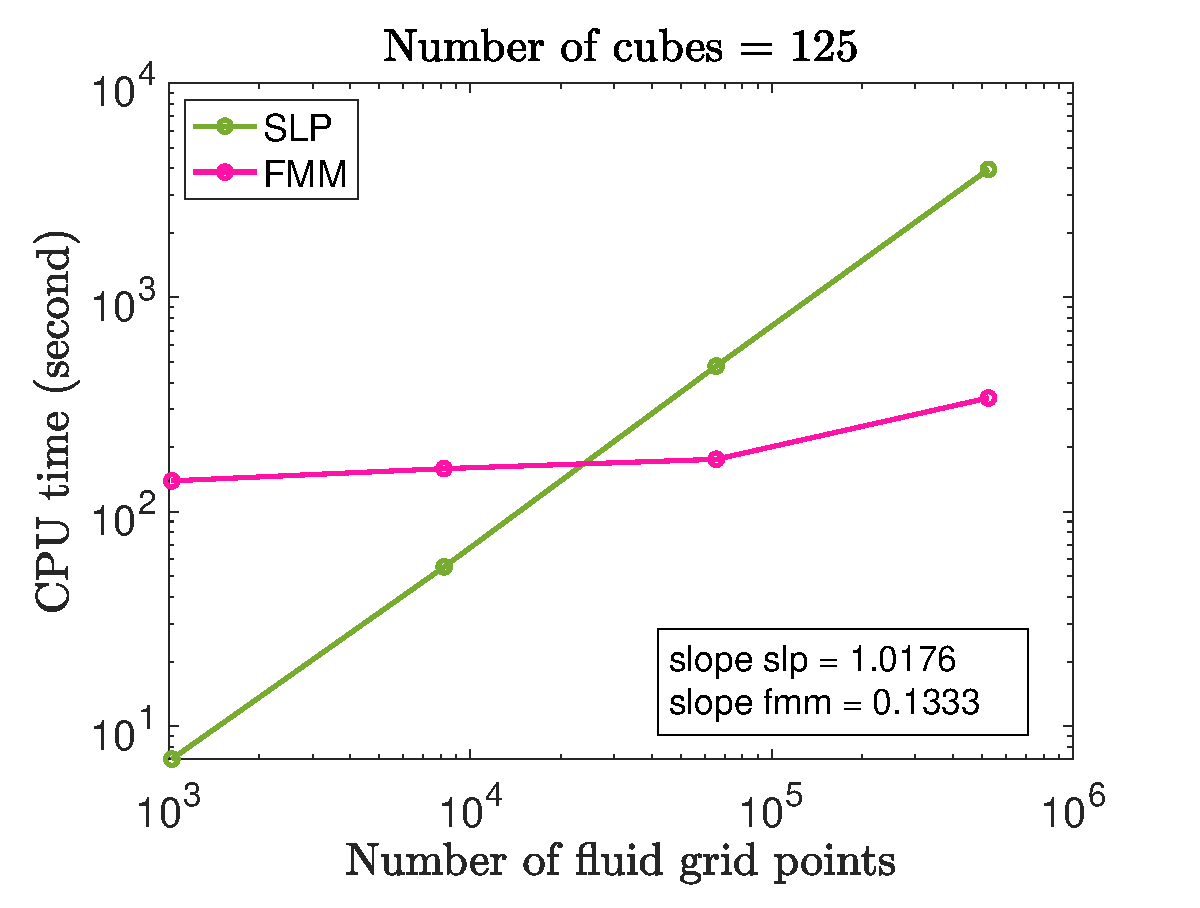
\includegraphics[scale=0.4]{./figures/fig_time_both_mm5_Nt10}
	\caption{(Left) Sample velocity plot at $t=1$ with $Nx = 2^6$. (Right) CPU time with an aggregate made with 125 cubes for 10 time steps. The Pinnacles is used.}
	\label{fig_vel_mm5_t1}
\end{center}
\end{figure}
\clearpage
On January 27, 2023, we decided to check in the timing and memory capacity to use the Pinnacles. I am going to test both SLP and FMM versions, separately, just to make sure if FMM is converging to the correct velocities. Here are the paratmesters we are going to use for this experiment:
\begin{framed}
	\begin{itemize}
	\item \verb+NC = [50, 100]+ (Random shape {\color{red}$\rightarrow$ check the Nf}) 
	\item \verb+Nx = [60, 120]+
	\item \verb+Ny = Nx, Nz = 2Nx+
	\item Fluid domain size: Make $\Delta x =\Delta y = \Delta z = 1$.
	\item $\Delta t = 0.5$
	\item \verb+Nt = 100+ (Final time would be 50.)
	\item Pe = 0.5 ( = $\Delta t$)
	\item {\color{blue} Save at 1) the final time only AND 2) every time step: velocity, C, $U_a$ with location, $\Omega$, $\theta$ (rotaion angle)}
	\end{itemize}
\end{framed}

\clearpage
Figure \ref{fig_time_fmm_sum} is Dec. 2022 results.
\begin{figure}[ht]
	\begin{center}
		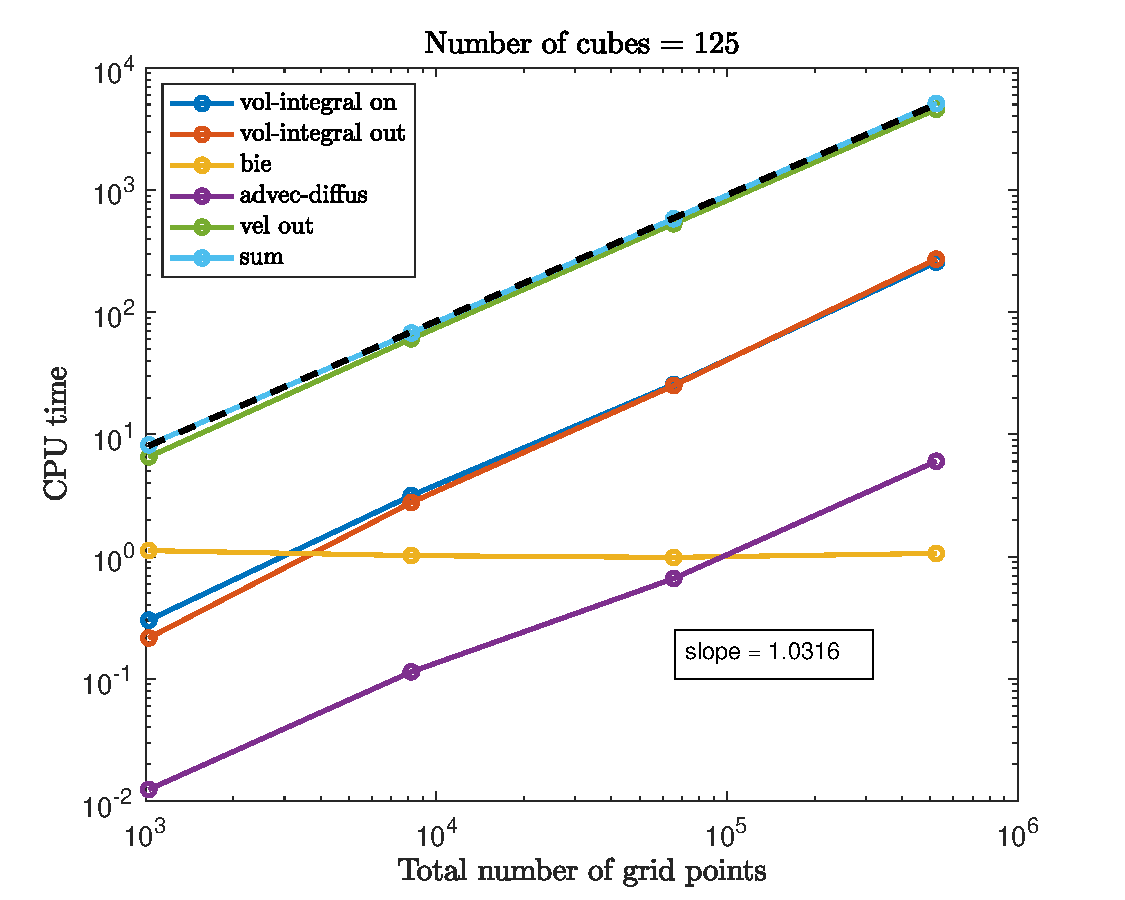
\includegraphics[scale=0.45]{./figures/fig_time_varNx5}
		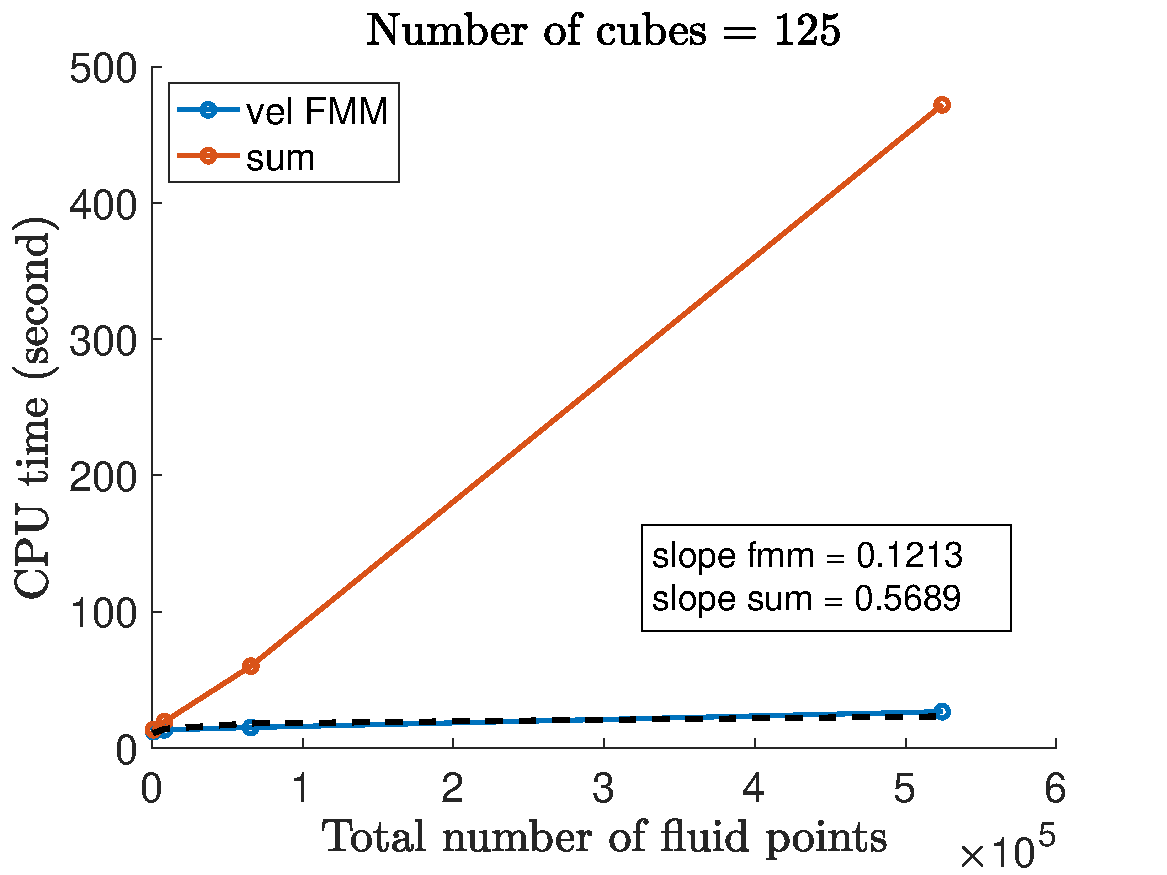
\includegraphics[scale=0.45]{./figures/fig_time_fmm_sum}
	\caption{CPU time with an aggregate made with 125 cubes for 10 time steps.}
	\label{fig_time_fmm_sum}
\end{center}
\end{figure}

% \begin{figure}[h]
% 	\begin{center}
% 		\vspace{0.5cm}
% 		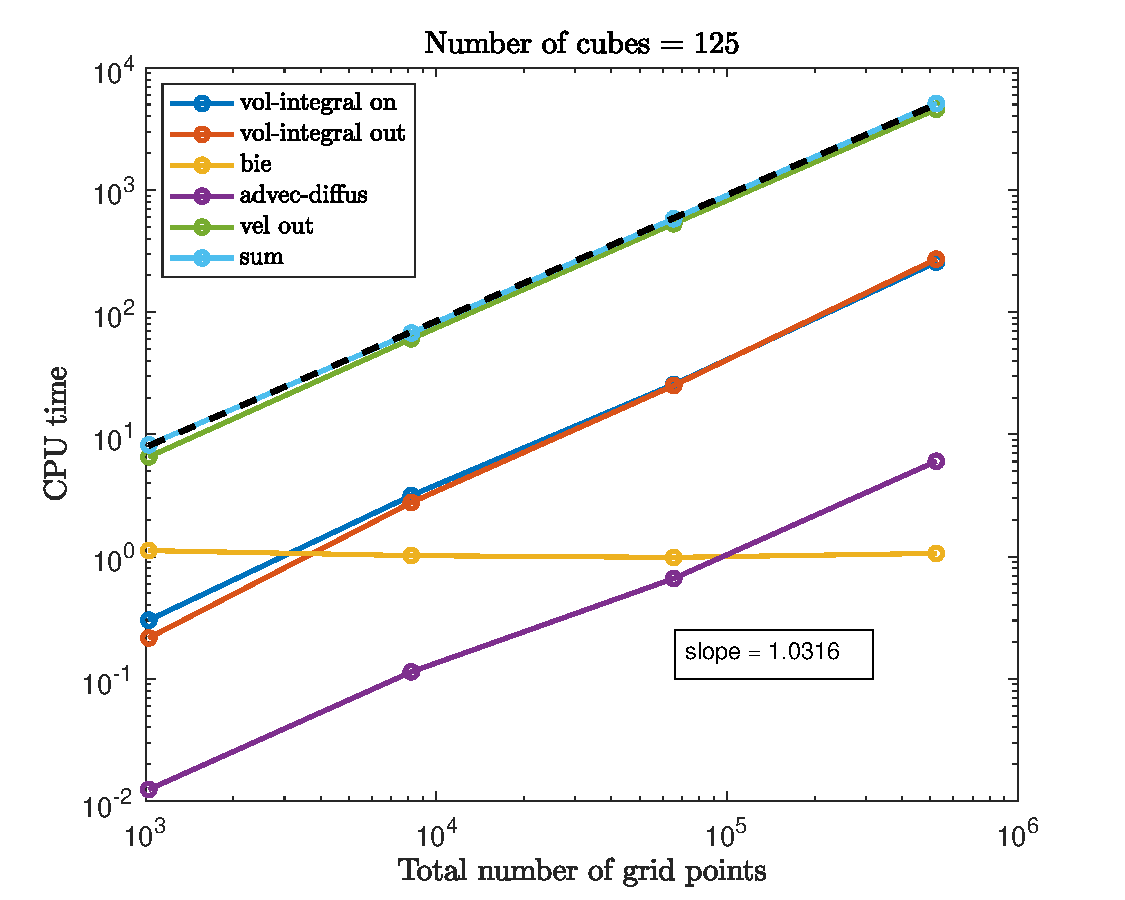
\includegraphics[scale=0.5]{./figures/fig_time_varNx5}	
% 	\caption{Number of cubes is 125.}
% 	\label{fig_time_varNx5}
% \end{center}
% \end{figure}
\begin{comment}
\clearpage
\begin{itemize}
	\item How did you code up exactly to use FMM3D?
	\item you may introduce index notations for this"  $i,j = 1,2,3$ works twice = 18 times  
	\item What is the main difference between volume integral and this surface integral?
	\item {\color{red} We expect to use total 18 times of FMM3D library to compute the entire velocity field.$\rightarrow$ why?}
\end{itemize}
In order to validate the code, measure the error size, and check the computation time, we consider a homogeneous case.
Error plots - compare the $U_a = -0.3470$ values.
\begin{figure}[h]
	\begin{center}
		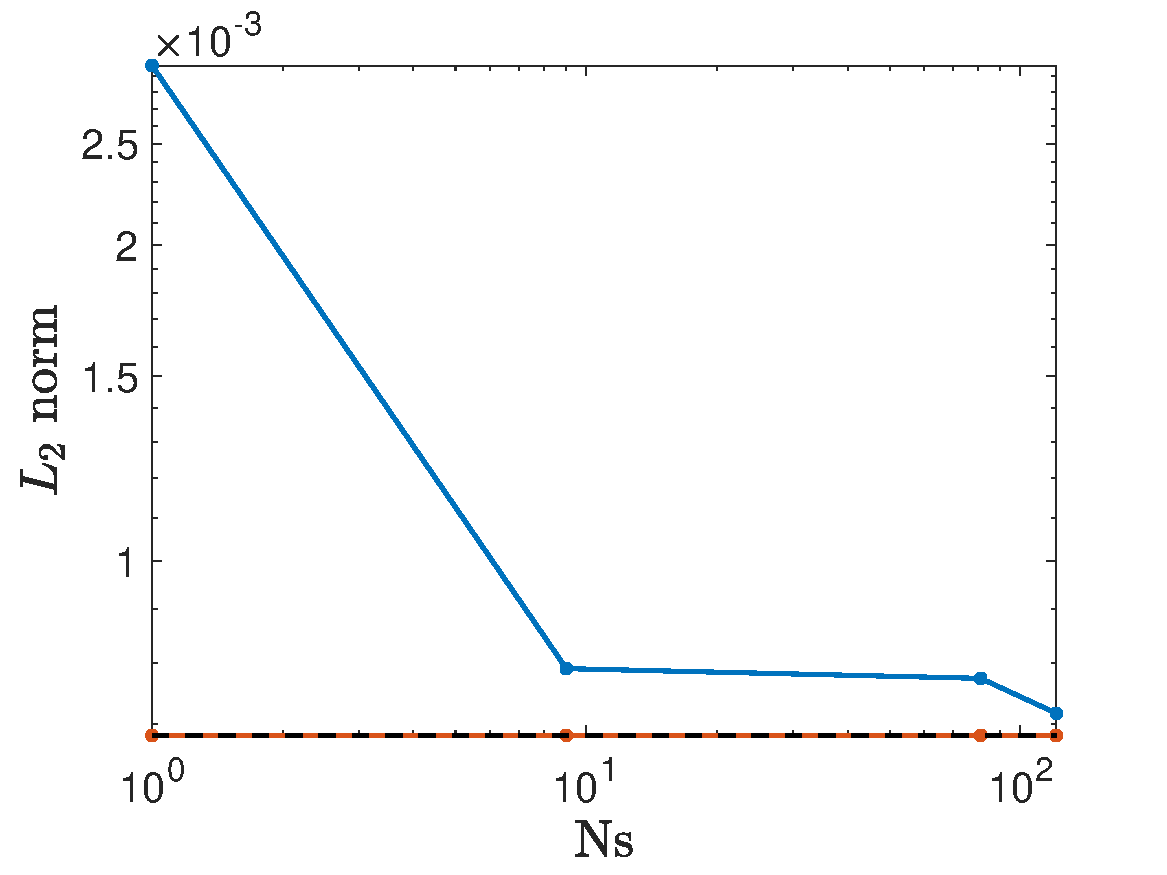
\includegraphics[scale=0.4]{./figures/fig_cornerErr_L2}
		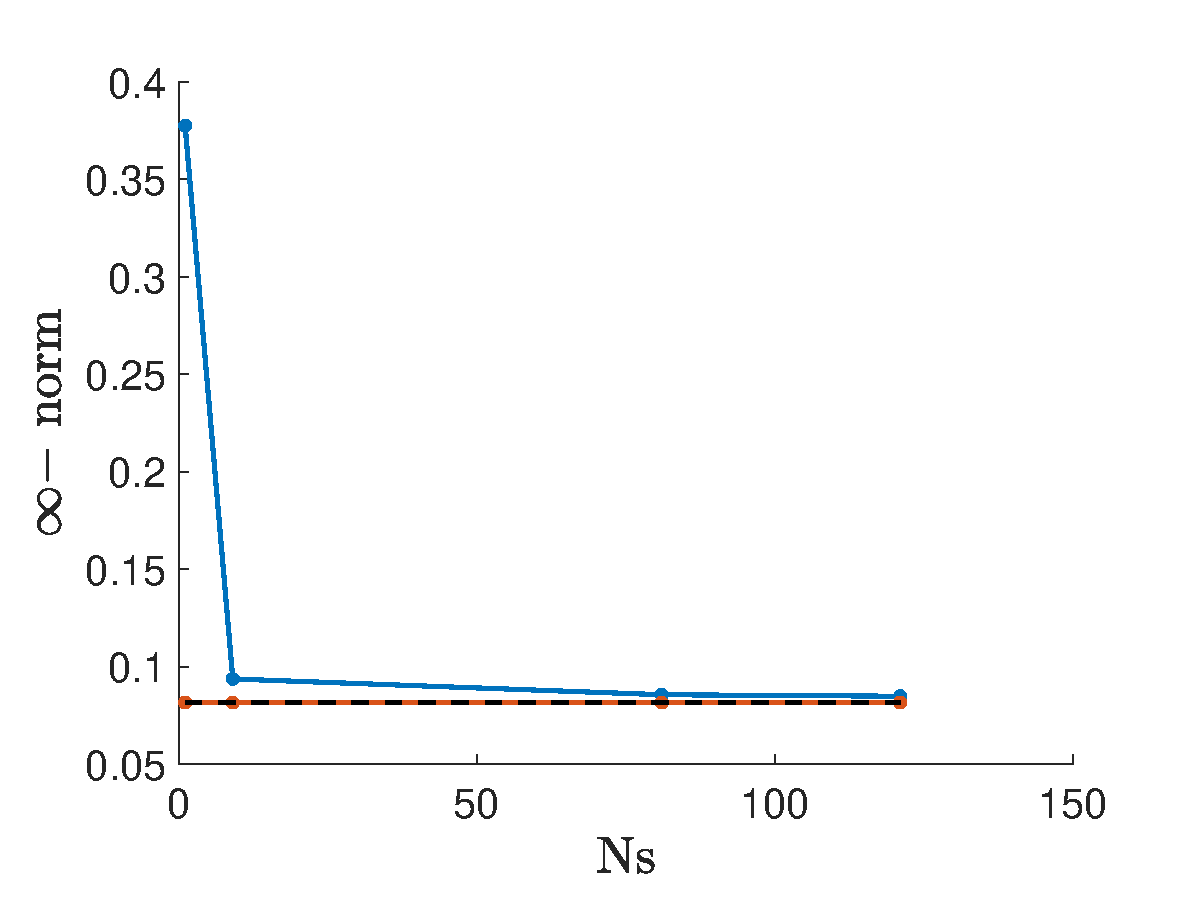
\includegraphics[scale=0.4]{./figures/fig_cornerErr_inf}
	\caption{(Left) Velocity plot of one face. 1 point is used to approximate the surface integral of $G$ kernel using FMM. (Right) $11^2$ point is used to approximate the surface integral of $G$ kernel using FMM. }
	\label{fig_cornerErr}
\end{center}
\end{figure}
\end{comment}
%Rotation---------------------------------------------------


\section{Numerical simulation results}
\section{Discussions}